% **************************************************************************************************************
% A Classic Thesis Style
% An Homage to The Elements of Typographic Style
%
% Copyright (C) 2015 André Miede http://www.miede.de
%
% If you like the style then I would appreciate a postcard. My address 
% can be found in the file ClassicThesis.pdf. A collection of the 
% postcards I received so far is available online at 
% http://postcards.miede.de
%
% License:
% This program is free software; you can redistribute it and/or modify
% it under the terms of the GNU General Public License as published by
% the Free Software Foundation; either version 2 of the License, or
% (at your option) any later version.
%
% This program is distributed in the hope that it will be useful,
% but WITHOUT ANY WARRANTY; without even the implied warranty of
% MERCHANTABILITY or FITNESS FOR A PARTICULAR PURPOSE.  See the
% GNU General Public License for more details.
%
% You should have received a copy of the GNU General Public License
% along with this program; see the file COPYING.  If not, write to
% the Free Software Foundation, Inc., 59 Temple Place - Suite 330,
% Boston, MA 02111-1307, USA.
%
% **************************************************************************************************************
\RequirePackage{fix-cm} % fix some latex issues see: http://texdoc.net/texmf-dist/doc/latex/base/fixltx2e.pdf
\documentclass[ twoside,openright,titlepage,numbers=noenddot,headinclude,%1headlines,% letterpaper a4paper
                footinclude=true,cleardoublepage=empty,abstractoff, % <--- obsolete, remove (todo)
                BCOR=5mm,paper=a4,fontsize=11pt,%11pt,a4paper,%
                ngerman,american,%
                ]{scrreprt}

%********************************************************************
% Note: Make all your adjustments in here
%*******************************************************
% ****************************************************************************************************
% classicthesis-config.tex 
% formerly known as loadpackages.sty, classicthesis-ldpkg.sty, and classicthesis-preamble.sty 
% Use it at the beginning of your ClassicThesis.tex, or as a LaTeX Preamble 
% in your ClassicThesis.{tex,lyx} with % ****************************************************************************************************
% classicthesis-config.tex 
% formerly known as loadpackages.sty, classicthesis-ldpkg.sty, and classicthesis-preamble.sty 
% Use it at the beginning of your ClassicThesis.tex, or as a LaTeX Preamble 
% in your ClassicThesis.{tex,lyx} with % ****************************************************************************************************
% classicthesis-config.tex 
% formerly known as loadpackages.sty, classicthesis-ldpkg.sty, and classicthesis-preamble.sty 
% Use it at the beginning of your ClassicThesis.tex, or as a LaTeX Preamble 
% in your ClassicThesis.{tex,lyx} with \input{classicthesis-config}
% ****************************************************************************************************  
% If you like the classicthesis, then I would appreciate a postcard. 
% My address can be found in the file ClassicThesis.pdf. A collection 
% of the postcards I received so far is available online at 
% http://postcards.miede.de
% ****************************************************************************************************


% ****************************************************************************************************
% 0. Set the encoding of your files. UTF-8 is the only sensible encoding nowadays. If you can't read
% äöüßáéçèê∂åëæƒÏ€ then change the encoding setting in your editor, not the line below. If your editor
% does not support utf8 use another editor!
% ****************************************************************************************************
\PassOptionsToPackage{utf8}{inputenc}
	\usepackage{inputenc}


\newcommand*\justify{%
	\fontdimen2\font=0.4em% interword space
	\fontdimen3\font=0.2em% interword stretch
	\fontdimen4\font=0.1em% interword shrink
	\fontdimen7\font=0.1em% extra space
	\hyphenchar\font=`\-% allowing hyphenation
}

\usepackage{dirtree}


% ****************************************************************************************************
% 1. Configure classicthesis for your needs here, e.g., remove "drafting" below 
% in order to deactivate the time-stamp on the pages
% ****************************************************************************************************
\PassOptionsToPackage{eulerchapternumbers,listings,%drafting,%
					 pdfspacing,%floatperchapter,%linedheaders,%
					 subfig,beramono,eulermath,parts,
				 	 dottedtoc}{classicthesis}                                        
% ********************************************************************
% Available options for classicthesis.sty 
% (see ClassicThesis.pdf for more information):
% drafting
% parts nochapters linedheaders
% eulerchapternumbers beramono eulermath pdfspacing minionprospacing
% tocaligned dottedtoc manychapters
% listings floatperchapter subfig
% ********************************************************************



% ****************************************************************************************************
% 2. Personal data and user ad-hoc commands
% ****************************************************************************************************
\newcommand{\myTitle}{Integración de Idemix en entornos de IoT\xspace}
\newcommand{\mySubtitle}{}
\newcommand{\myDegree}{}%Doktor-Ingenieur (Dr.-Ing.)\xspace}
\newcommand{\myName}{José Luis Cánovas Sánchez\xspace}
\newcommand{\myProf}{Antonio Fernando Skarmeta Gómez\xspace}
\newcommand{\myOtherProf}{Jorge Bernal Bernabé\xspace}
\newcommand{\mySupervisor}{}%Put name here\xspace}
\newcommand{\myFaculty}{Facultad de Ingeniería Informática\xspace}
\newcommand{\myDepartment}{}%Put data here\xspace}
\newcommand{\myUni}{Universidad de Murcia\xspace}
\newcommand{\myLocation}{Murcia}%Saarbrücken\xspace}
\newcommand{\myTime}{Junio 2017}%September 2015\xspace}
\newcommand{\myVersion}{}%version 4.2\xspace}

% ********************************************************************
% Setup, finetuning, and useful commands
% ********************************************************************
\newcounter{dummy} % necessary for correct hyperlinks (to index, bib, etc.)
\newlength{\abcd} % for ab..z string length calculation
\providecommand{\mLyX}{L\kern-.1667em\lower.25em\hbox{Y}\kern-.125emX\@}
\newcommand{\ie}{i.\,e.}
\newcommand{\Ie}{I.\,e.}
\newcommand{\eg}{e.\,g.}
\newcommand{\Eg}{E.\,g.} 
% ****************************************************************************************************


% ****************************************************************************************************
% 3. Loading some handy packages
% ****************************************************************************************************
% ******************************************************************** 
% Packages with options that might require adjustments
% ******************************************************************** 
%\PassOptionsToPackage{ngerman,american}{babel}   % change this to your language(s)
% Spanish languages need extra options in order to work with this template
%\PassOptionsToPackage{spanish,es-lcroman}{babel}
	\usepackage{babel}                  

\usepackage{csquotes}
\PassOptionsToPackage{%
    %backend=biber, %instead of bibtex
	backend=bibtex8,bibencoding=ascii,%
	language=auto,%
	style=numeric-comp,%
    %style=authoryear-comp, % Author 1999, 2010
    %bibstyle=authoryear,dashed=false, % dashed: substitute rep. author with ---
    sorting=nyt, % name, year, title
    maxbibnames=10, % default: 3, et al.
    %backref=true,%
    natbib=true % natbib compatibility mode (\citep and \citet still work)
}{biblatex}
    \usepackage{biblatex}

\PassOptionsToPackage{fleqn}{amsmath}       % math environments and more by the AMS 
    \usepackage{amsmath}

% ******************************************************************** 
% General useful packages
% ******************************************************************** 
\PassOptionsToPackage{T1}{fontenc} % T2A for cyrillics
    \usepackage{fontenc}     
\usepackage{textcomp} % fix warning with missing font shapes
\usepackage{scrhack} % fix warnings when using KOMA with listings package          
\usepackage{xspace} % to get the spacing after macros right  
\usepackage{mparhack} % get marginpar right
\usepackage{fixltx2e} % fixes some LaTeX stuff --> since 2015 in the LaTeX kernel (see below)
%\usepackage[latest]{latexrelease} % will be used once available in more distributions (ISSUE #107)
\PassOptionsToPackage{printonlyused,smaller}{acronym} 
    \usepackage{acronym} % nice macros for handling all acronyms in the thesis
    %\renewcommand{\bflabel}[1]{{#1}\hfill} % fix the list of acronyms --> no longer working
    %\renewcommand*{\acsfont}[1]{\textsc{#1}} 
    \renewcommand*{\aclabelfont}[1]{\acsfont{#1}}
% ****************************************************************************************************


% ****************************************************************************************************
% 4. Setup floats: tables, (sub)figures, and captions
% ****************************************************************************************************
\usepackage{tabularx} % better tables
    \setlength{\extrarowheight}{3pt} % increase table row height
\newcommand{\tableheadline}[1]{\multicolumn{1}{c}{\spacedlowsmallcaps{#1}}}
\newcommand{\myfloatalign}{\centering} % to be used with each float for alignment
\usepackage{caption}
% Thanks to cgnieder and Claus Lahiri
% http://tex.stackexchange.com/questions/69349/spacedlowsmallcaps-in-caption-label
% [REMOVED DUE TO OTHER PROBLEMS, SEE ISSUE #82]    
%\DeclareCaptionLabelFormat{smallcaps}{\bothIfFirst{#1}{~}\MakeTextLowercase{\textsc{#2}}}
%\captionsetup{font=small,labelformat=smallcaps} % format=hang,
\captionsetup{font=small} % format=hang,
\usepackage{subfig}  
% ****************************************************************************************************


% ****************************************************************************************************
% 5. Setup code listings
% ****************************************************************************************************
\usepackage{listings} 
%\lstset{emph={trueIndex,root},emphstyle=\color{BlueViolet}}%\underbar} % for special keywords
\lstset{language=[LaTeX]Tex,%C++,
    morekeywords={PassOptionsToPackage,selectlanguage},
    keywordstyle=\color{RoyalBlue},%\bfseries,
    basicstyle=\small\ttfamily,
    %identifierstyle=\color{NavyBlue},
    commentstyle=\color{Green}\ttfamily,
    stringstyle=\rmfamily,
    numbers=none,%left,%
    numberstyle=\scriptsize,%\tiny
    stepnumber=5,
    numbersep=8pt,
    showstringspaces=false,
    breaklines=true,
    %frameround=ftff,
    %frame=single,
    belowcaptionskip=.75\baselineskip
    %frame=L
} 
% ****************************************************************************************************             


% ****************************************************************************************************
% 6. PDFLaTeX, hyperreferences and citation backreferences
% ****************************************************************************************************
% ********************************************************************
% Using PDFLaTeX
% ********************************************************************
\PassOptionsToPackage{pdftex,hyperfootnotes=false,pdfpagelabels}{hyperref}
    \usepackage{hyperref}  % backref linktocpage pagebackref
\pdfcompresslevel=9
\pdfadjustspacing=1 
\PassOptionsToPackage{pdftex}{graphicx}
    \usepackage{graphicx} 
 

% ********************************************************************
% Hyperreferences
% ********************************************************************
\hypersetup{%
    %draft, % = no hyperlinking at all (useful in b/w printouts)
    colorlinks=true, linktocpage=true, pdfstartpage=1, pdfstartview=FitV,%
    % uncomment the following line if you want to have black links (e.g., for printing)
    %colorlinks=false, linktocpage=false, pdfstartpage=3, pdfstartview=FitV, pdfborder={0 0 0},%
    breaklinks=true, pdfpagemode=UseNone, pageanchor=true, pdfpagemode=UseOutlines,%
    plainpages=false, bookmarksnumbered, bookmarksopen=true, bookmarksopenlevel=1,%
    hypertexnames=true, pdfhighlight=/O,%nesting=true,%frenchlinks,%
    urlcolor=webbrown, linkcolor=RoyalBlue, citecolor=webgreen, %pagecolor=RoyalBlue,%
    %urlcolor=Black, linkcolor=Black, citecolor=Black, %pagecolor=Black,%
    pdftitle={\myTitle},%
    pdfauthor={\textcopyright\ \myName, \myUni, \myFaculty},%
    pdfsubject={},%
    pdfkeywords={},%
    pdfcreator={pdfLaTeX},%
    pdfproducer={LaTeX with hyperref and classicthesis}%
}   

% ********************************************************************
% Setup autoreferences
% ********************************************************************
% There are some issues regarding autorefnames
% http://www.ureader.de/msg/136221647.aspx
% http://www.tex.ac.uk/cgi-bin/texfaq2html?label=latexwords
% you have to redefine the makros for the 
% language you use, e.g., american, ngerman
% (as chosen when loading babel/AtBeginDocument)
% ********************************************************************
\makeatletter
\@ifpackageloaded{babel}%
    {%
       \addto\extrasamerican{%
			\renewcommand*{\figureautorefname}{Figure}%
			\renewcommand*{\tableautorefname}{Table}%
			\renewcommand*{\partautorefname}{Part}%
			\renewcommand*{\chapterautorefname}{Chapter}%
			\renewcommand*{\sectionautorefname}{Section}%
			\renewcommand*{\subsectionautorefname}{Section}%
			\renewcommand*{\subsubsectionautorefname}{Section}%     
                }%
       \addto\extrasngerman{% 
			\renewcommand*{\paragraphautorefname}{Absatz}%
			\renewcommand*{\subparagraphautorefname}{Unterabsatz}%
			\renewcommand*{\footnoteautorefname}{Fu\"snote}%
			\renewcommand*{\FancyVerbLineautorefname}{Zeile}%
			\renewcommand*{\theoremautorefname}{Theorem}%
			\renewcommand*{\appendixautorefname}{Anhang}%
			\renewcommand*{\equationautorefname}{Gleichung}%        
			\renewcommand*{\itemautorefname}{Punkt}%
                }%  
            % Fix to getting autorefs for subfigures right (thanks to Belinda Vogt for changing the definition)
            \providecommand{\subfigureautorefname}{\figureautorefname}%             
    }{\relax}
\makeatother


% ****************************************************************************************************
% 7. Last calls before the bar closes
% ****************************************************************************************************
% ********************************************************************
% Development Stuff
% ********************************************************************
\listfiles
%\PassOptionsToPackage{l2tabu,orthodox,abort}{nag}
%   \usepackage{nag}
%\PassOptionsToPackage{warning, all}{onlyamsmath}
%   \usepackage{onlyamsmath}

% ********************************************************************
% Last, but not least...
% ********************************************************************
\usepackage{classicthesis} 
% ****************************************************************************************************


% ****************************************************************************************************
% 8. Further adjustments (experimental)
% ****************************************************************************************************
% ********************************************************************
% Changing the text area
% ********************************************************************
\linespread{1.05} % a bit more for Palatino
%\areaset[current]{312pt}{761pt} % 686 (factor 2.2) + 33 head + 42 head \the\footskip
%\setlength{\marginparwidth}{7em}%
%\setlength{\marginparsep}{2em}%

% ********************************************************************
% Using different fonts
% ********************************************************************
%\usepackage[oldstylenums]{kpfonts} % oldstyle notextcomp
%\usepackage[osf]{libertine}
%\usepackage[light,condensed,math]{iwona}
%\renewcommand{\sfdefault}{iwona}
%\usepackage{lmodern} % <-- no osf support :-(
%\usepackage{cfr-lm} % 
%\usepackage[urw-garamond]{mathdesign} <-- no osf support :-(
%\usepackage[default,osfigures]{opensans} % scale=0.95 
%\usepackage[sfdefault]{FiraSans}
% ****************************************************************************************************

% ****************************************************************************************************  
% If you like the classicthesis, then I would appreciate a postcard. 
% My address can be found in the file ClassicThesis.pdf. A collection 
% of the postcards I received so far is available online at 
% http://postcards.miede.de
% ****************************************************************************************************


% ****************************************************************************************************
% 0. Set the encoding of your files. UTF-8 is the only sensible encoding nowadays. If you can't read
% äöüßáéçèê∂åëæƒÏ€ then change the encoding setting in your editor, not the line below. If your editor
% does not support utf8 use another editor!
% ****************************************************************************************************
\PassOptionsToPackage{utf8}{inputenc}
	\usepackage{inputenc}


\newcommand*\justify{%
	\fontdimen2\font=0.4em% interword space
	\fontdimen3\font=0.2em% interword stretch
	\fontdimen4\font=0.1em% interword shrink
	\fontdimen7\font=0.1em% extra space
	\hyphenchar\font=`\-% allowing hyphenation
}

\usepackage{dirtree}


% ****************************************************************************************************
% 1. Configure classicthesis for your needs here, e.g., remove "drafting" below 
% in order to deactivate the time-stamp on the pages
% ****************************************************************************************************
\PassOptionsToPackage{eulerchapternumbers,listings,%drafting,%
					 pdfspacing,%floatperchapter,%linedheaders,%
					 subfig,beramono,eulermath,parts,
				 	 dottedtoc}{classicthesis}                                        
% ********************************************************************
% Available options for classicthesis.sty 
% (see ClassicThesis.pdf for more information):
% drafting
% parts nochapters linedheaders
% eulerchapternumbers beramono eulermath pdfspacing minionprospacing
% tocaligned dottedtoc manychapters
% listings floatperchapter subfig
% ********************************************************************



% ****************************************************************************************************
% 2. Personal data and user ad-hoc commands
% ****************************************************************************************************
\newcommand{\myTitle}{Integración de Idemix en entornos de IoT\xspace}
\newcommand{\mySubtitle}{}
\newcommand{\myDegree}{}%Doktor-Ingenieur (Dr.-Ing.)\xspace}
\newcommand{\myName}{José Luis Cánovas Sánchez\xspace}
\newcommand{\myProf}{Antonio Fernando Skarmeta Gómez\xspace}
\newcommand{\myOtherProf}{Jorge Bernal Bernabé\xspace}
\newcommand{\mySupervisor}{}%Put name here\xspace}
\newcommand{\myFaculty}{Facultad de Ingeniería Informática\xspace}
\newcommand{\myDepartment}{}%Put data here\xspace}
\newcommand{\myUni}{Universidad de Murcia\xspace}
\newcommand{\myLocation}{Murcia}%Saarbrücken\xspace}
\newcommand{\myTime}{Junio 2017}%September 2015\xspace}
\newcommand{\myVersion}{}%version 4.2\xspace}

% ********************************************************************
% Setup, finetuning, and useful commands
% ********************************************************************
\newcounter{dummy} % necessary for correct hyperlinks (to index, bib, etc.)
\newlength{\abcd} % for ab..z string length calculation
\providecommand{\mLyX}{L\kern-.1667em\lower.25em\hbox{Y}\kern-.125emX\@}
\newcommand{\ie}{i.\,e.}
\newcommand{\Ie}{I.\,e.}
\newcommand{\eg}{e.\,g.}
\newcommand{\Eg}{E.\,g.} 
% ****************************************************************************************************


% ****************************************************************************************************
% 3. Loading some handy packages
% ****************************************************************************************************
% ******************************************************************** 
% Packages with options that might require adjustments
% ******************************************************************** 
%\PassOptionsToPackage{ngerman,american}{babel}   % change this to your language(s)
% Spanish languages need extra options in order to work with this template
%\PassOptionsToPackage{spanish,es-lcroman}{babel}
	\usepackage{babel}                  

\usepackage{csquotes}
\PassOptionsToPackage{%
    %backend=biber, %instead of bibtex
	backend=bibtex8,bibencoding=ascii,%
	language=auto,%
	style=numeric-comp,%
    %style=authoryear-comp, % Author 1999, 2010
    %bibstyle=authoryear,dashed=false, % dashed: substitute rep. author with ---
    sorting=nyt, % name, year, title
    maxbibnames=10, % default: 3, et al.
    %backref=true,%
    natbib=true % natbib compatibility mode (\citep and \citet still work)
}{biblatex}
    \usepackage{biblatex}

\PassOptionsToPackage{fleqn}{amsmath}       % math environments and more by the AMS 
    \usepackage{amsmath}

% ******************************************************************** 
% General useful packages
% ******************************************************************** 
\PassOptionsToPackage{T1}{fontenc} % T2A for cyrillics
    \usepackage{fontenc}     
\usepackage{textcomp} % fix warning with missing font shapes
\usepackage{scrhack} % fix warnings when using KOMA with listings package          
\usepackage{xspace} % to get the spacing after macros right  
\usepackage{mparhack} % get marginpar right
\usepackage{fixltx2e} % fixes some LaTeX stuff --> since 2015 in the LaTeX kernel (see below)
%\usepackage[latest]{latexrelease} % will be used once available in more distributions (ISSUE #107)
\PassOptionsToPackage{printonlyused,smaller}{acronym} 
    \usepackage{acronym} % nice macros for handling all acronyms in the thesis
    %\renewcommand{\bflabel}[1]{{#1}\hfill} % fix the list of acronyms --> no longer working
    %\renewcommand*{\acsfont}[1]{\textsc{#1}} 
    \renewcommand*{\aclabelfont}[1]{\acsfont{#1}}
% ****************************************************************************************************


% ****************************************************************************************************
% 4. Setup floats: tables, (sub)figures, and captions
% ****************************************************************************************************
\usepackage{tabularx} % better tables
    \setlength{\extrarowheight}{3pt} % increase table row height
\newcommand{\tableheadline}[1]{\multicolumn{1}{c}{\spacedlowsmallcaps{#1}}}
\newcommand{\myfloatalign}{\centering} % to be used with each float for alignment
\usepackage{caption}
% Thanks to cgnieder and Claus Lahiri
% http://tex.stackexchange.com/questions/69349/spacedlowsmallcaps-in-caption-label
% [REMOVED DUE TO OTHER PROBLEMS, SEE ISSUE #82]    
%\DeclareCaptionLabelFormat{smallcaps}{\bothIfFirst{#1}{~}\MakeTextLowercase{\textsc{#2}}}
%\captionsetup{font=small,labelformat=smallcaps} % format=hang,
\captionsetup{font=small} % format=hang,
\usepackage{subfig}  
% ****************************************************************************************************


% ****************************************************************************************************
% 5. Setup code listings
% ****************************************************************************************************
\usepackage{listings} 
%\lstset{emph={trueIndex,root},emphstyle=\color{BlueViolet}}%\underbar} % for special keywords
\lstset{language=[LaTeX]Tex,%C++,
    morekeywords={PassOptionsToPackage,selectlanguage},
    keywordstyle=\color{RoyalBlue},%\bfseries,
    basicstyle=\small\ttfamily,
    %identifierstyle=\color{NavyBlue},
    commentstyle=\color{Green}\ttfamily,
    stringstyle=\rmfamily,
    numbers=none,%left,%
    numberstyle=\scriptsize,%\tiny
    stepnumber=5,
    numbersep=8pt,
    showstringspaces=false,
    breaklines=true,
    %frameround=ftff,
    %frame=single,
    belowcaptionskip=.75\baselineskip
    %frame=L
} 
% ****************************************************************************************************             


% ****************************************************************************************************
% 6. PDFLaTeX, hyperreferences and citation backreferences
% ****************************************************************************************************
% ********************************************************************
% Using PDFLaTeX
% ********************************************************************
\PassOptionsToPackage{pdftex,hyperfootnotes=false,pdfpagelabels}{hyperref}
    \usepackage{hyperref}  % backref linktocpage pagebackref
\pdfcompresslevel=9
\pdfadjustspacing=1 
\PassOptionsToPackage{pdftex}{graphicx}
    \usepackage{graphicx} 
 

% ********************************************************************
% Hyperreferences
% ********************************************************************
\hypersetup{%
    %draft, % = no hyperlinking at all (useful in b/w printouts)
    colorlinks=true, linktocpage=true, pdfstartpage=1, pdfstartview=FitV,%
    % uncomment the following line if you want to have black links (e.g., for printing)
    %colorlinks=false, linktocpage=false, pdfstartpage=3, pdfstartview=FitV, pdfborder={0 0 0},%
    breaklinks=true, pdfpagemode=UseNone, pageanchor=true, pdfpagemode=UseOutlines,%
    plainpages=false, bookmarksnumbered, bookmarksopen=true, bookmarksopenlevel=1,%
    hypertexnames=true, pdfhighlight=/O,%nesting=true,%frenchlinks,%
    urlcolor=webbrown, linkcolor=RoyalBlue, citecolor=webgreen, %pagecolor=RoyalBlue,%
    %urlcolor=Black, linkcolor=Black, citecolor=Black, %pagecolor=Black,%
    pdftitle={\myTitle},%
    pdfauthor={\textcopyright\ \myName, \myUni, \myFaculty},%
    pdfsubject={},%
    pdfkeywords={},%
    pdfcreator={pdfLaTeX},%
    pdfproducer={LaTeX with hyperref and classicthesis}%
}   

% ********************************************************************
% Setup autoreferences
% ********************************************************************
% There are some issues regarding autorefnames
% http://www.ureader.de/msg/136221647.aspx
% http://www.tex.ac.uk/cgi-bin/texfaq2html?label=latexwords
% you have to redefine the makros for the 
% language you use, e.g., american, ngerman
% (as chosen when loading babel/AtBeginDocument)
% ********************************************************************
\makeatletter
\@ifpackageloaded{babel}%
    {%
       \addto\extrasamerican{%
			\renewcommand*{\figureautorefname}{Figure}%
			\renewcommand*{\tableautorefname}{Table}%
			\renewcommand*{\partautorefname}{Part}%
			\renewcommand*{\chapterautorefname}{Chapter}%
			\renewcommand*{\sectionautorefname}{Section}%
			\renewcommand*{\subsectionautorefname}{Section}%
			\renewcommand*{\subsubsectionautorefname}{Section}%     
                }%
       \addto\extrasngerman{% 
			\renewcommand*{\paragraphautorefname}{Absatz}%
			\renewcommand*{\subparagraphautorefname}{Unterabsatz}%
			\renewcommand*{\footnoteautorefname}{Fu\"snote}%
			\renewcommand*{\FancyVerbLineautorefname}{Zeile}%
			\renewcommand*{\theoremautorefname}{Theorem}%
			\renewcommand*{\appendixautorefname}{Anhang}%
			\renewcommand*{\equationautorefname}{Gleichung}%        
			\renewcommand*{\itemautorefname}{Punkt}%
                }%  
            % Fix to getting autorefs for subfigures right (thanks to Belinda Vogt for changing the definition)
            \providecommand{\subfigureautorefname}{\figureautorefname}%             
    }{\relax}
\makeatother


% ****************************************************************************************************
% 7. Last calls before the bar closes
% ****************************************************************************************************
% ********************************************************************
% Development Stuff
% ********************************************************************
\listfiles
%\PassOptionsToPackage{l2tabu,orthodox,abort}{nag}
%   \usepackage{nag}
%\PassOptionsToPackage{warning, all}{onlyamsmath}
%   \usepackage{onlyamsmath}

% ********************************************************************
% Last, but not least...
% ********************************************************************
\usepackage{classicthesis} 
% ****************************************************************************************************


% ****************************************************************************************************
% 8. Further adjustments (experimental)
% ****************************************************************************************************
% ********************************************************************
% Changing the text area
% ********************************************************************
\linespread{1.05} % a bit more for Palatino
%\areaset[current]{312pt}{761pt} % 686 (factor 2.2) + 33 head + 42 head \the\footskip
%\setlength{\marginparwidth}{7em}%
%\setlength{\marginparsep}{2em}%

% ********************************************************************
% Using different fonts
% ********************************************************************
%\usepackage[oldstylenums]{kpfonts} % oldstyle notextcomp
%\usepackage[osf]{libertine}
%\usepackage[light,condensed,math]{iwona}
%\renewcommand{\sfdefault}{iwona}
%\usepackage{lmodern} % <-- no osf support :-(
%\usepackage{cfr-lm} % 
%\usepackage[urw-garamond]{mathdesign} <-- no osf support :-(
%\usepackage[default,osfigures]{opensans} % scale=0.95 
%\usepackage[sfdefault]{FiraSans}
% ****************************************************************************************************

% ****************************************************************************************************  
% If you like the classicthesis, then I would appreciate a postcard. 
% My address can be found in the file ClassicThesis.pdf. A collection 
% of the postcards I received so far is available online at 
% http://postcards.miede.de
% ****************************************************************************************************


% ****************************************************************************************************
% 0. Set the encoding of your files. UTF-8 is the only sensible encoding nowadays. If you can't read
% äöüßáéçèê∂åëæƒÏ€ then change the encoding setting in your editor, not the line below. If your editor
% does not support utf8 use another editor!
% ****************************************************************************************************
\PassOptionsToPackage{utf8}{inputenc}
	\usepackage{inputenc}


\newcommand*\justify{%
	\fontdimen2\font=0.4em% interword space
	\fontdimen3\font=0.2em% interword stretch
	\fontdimen4\font=0.1em% interword shrink
	\fontdimen7\font=0.1em% extra space
	\hyphenchar\font=`\-% allowing hyphenation
}

\usepackage{dirtree}


% ****************************************************************************************************
% 1. Configure classicthesis for your needs here, e.g., remove "drafting" below 
% in order to deactivate the time-stamp on the pages
% ****************************************************************************************************
\PassOptionsToPackage{eulerchapternumbers,listings,%drafting,%
					 pdfspacing,%floatperchapter,%linedheaders,%
					 subfig,beramono,eulermath,parts,
				 	 dottedtoc}{classicthesis}                                        
% ********************************************************************
% Available options for classicthesis.sty 
% (see ClassicThesis.pdf for more information):
% drafting
% parts nochapters linedheaders
% eulerchapternumbers beramono eulermath pdfspacing minionprospacing
% tocaligned dottedtoc manychapters
% listings floatperchapter subfig
% ********************************************************************



% ****************************************************************************************************
% 2. Personal data and user ad-hoc commands
% ****************************************************************************************************
\newcommand{\myTitle}{Integración de Idemix en entornos de IoT\xspace}
\newcommand{\mySubtitle}{}
\newcommand{\myDegree}{}%Doktor-Ingenieur (Dr.-Ing.)\xspace}
\newcommand{\myName}{José Luis Cánovas Sánchez\xspace}
\newcommand{\myProf}{Antonio Fernando Skarmeta Gómez\xspace}
\newcommand{\myOtherProf}{Jorge Bernal Bernabé\xspace}
\newcommand{\mySupervisor}{}%Put name here\xspace}
\newcommand{\myFaculty}{Facultad de Ingeniería Informática\xspace}
\newcommand{\myDepartment}{}%Put data here\xspace}
\newcommand{\myUni}{Universidad de Murcia\xspace}
\newcommand{\myLocation}{Murcia}%Saarbrücken\xspace}
\newcommand{\myTime}{Junio 2017}%September 2015\xspace}
\newcommand{\myVersion}{}%version 4.2\xspace}

% ********************************************************************
% Setup, finetuning, and useful commands
% ********************************************************************
\newcounter{dummy} % necessary for correct hyperlinks (to index, bib, etc.)
\newlength{\abcd} % for ab..z string length calculation
\providecommand{\mLyX}{L\kern-.1667em\lower.25em\hbox{Y}\kern-.125emX\@}
\newcommand{\ie}{i.\,e.}
\newcommand{\Ie}{I.\,e.}
\newcommand{\eg}{e.\,g.}
\newcommand{\Eg}{E.\,g.} 
% ****************************************************************************************************


% ****************************************************************************************************
% 3. Loading some handy packages
% ****************************************************************************************************
% ******************************************************************** 
% Packages with options that might require adjustments
% ******************************************************************** 
%\PassOptionsToPackage{ngerman,american}{babel}   % change this to your language(s)
% Spanish languages need extra options in order to work with this template
%\PassOptionsToPackage{spanish,es-lcroman}{babel}
	\usepackage{babel}                  

\usepackage{csquotes}
\PassOptionsToPackage{%
    %backend=biber, %instead of bibtex
	backend=bibtex8,bibencoding=ascii,%
	language=auto,%
	style=numeric-comp,%
    %style=authoryear-comp, % Author 1999, 2010
    %bibstyle=authoryear,dashed=false, % dashed: substitute rep. author with ---
    sorting=nyt, % name, year, title
    maxbibnames=10, % default: 3, et al.
    %backref=true,%
    natbib=true % natbib compatibility mode (\citep and \citet still work)
}{biblatex}
    \usepackage{biblatex}

\PassOptionsToPackage{fleqn}{amsmath}       % math environments and more by the AMS 
    \usepackage{amsmath}

% ******************************************************************** 
% General useful packages
% ******************************************************************** 
\PassOptionsToPackage{T1}{fontenc} % T2A for cyrillics
    \usepackage{fontenc}     
\usepackage{textcomp} % fix warning with missing font shapes
\usepackage{scrhack} % fix warnings when using KOMA with listings package          
\usepackage{xspace} % to get the spacing after macros right  
\usepackage{mparhack} % get marginpar right
\usepackage{fixltx2e} % fixes some LaTeX stuff --> since 2015 in the LaTeX kernel (see below)
%\usepackage[latest]{latexrelease} % will be used once available in more distributions (ISSUE #107)
\PassOptionsToPackage{printonlyused,smaller}{acronym} 
    \usepackage{acronym} % nice macros for handling all acronyms in the thesis
    %\renewcommand{\bflabel}[1]{{#1}\hfill} % fix the list of acronyms --> no longer working
    %\renewcommand*{\acsfont}[1]{\textsc{#1}} 
    \renewcommand*{\aclabelfont}[1]{\acsfont{#1}}
% ****************************************************************************************************


% ****************************************************************************************************
% 4. Setup floats: tables, (sub)figures, and captions
% ****************************************************************************************************
\usepackage{tabularx} % better tables
    \setlength{\extrarowheight}{3pt} % increase table row height
\newcommand{\tableheadline}[1]{\multicolumn{1}{c}{\spacedlowsmallcaps{#1}}}
\newcommand{\myfloatalign}{\centering} % to be used with each float for alignment
\usepackage{caption}
% Thanks to cgnieder and Claus Lahiri
% http://tex.stackexchange.com/questions/69349/spacedlowsmallcaps-in-caption-label
% [REMOVED DUE TO OTHER PROBLEMS, SEE ISSUE #82]    
%\DeclareCaptionLabelFormat{smallcaps}{\bothIfFirst{#1}{~}\MakeTextLowercase{\textsc{#2}}}
%\captionsetup{font=small,labelformat=smallcaps} % format=hang,
\captionsetup{font=small} % format=hang,
\usepackage{subfig}  
% ****************************************************************************************************


% ****************************************************************************************************
% 5. Setup code listings
% ****************************************************************************************************
\usepackage{listings} 
%\lstset{emph={trueIndex,root},emphstyle=\color{BlueViolet}}%\underbar} % for special keywords
\lstset{language=[LaTeX]Tex,%C++,
    morekeywords={PassOptionsToPackage,selectlanguage},
    keywordstyle=\color{RoyalBlue},%\bfseries,
    basicstyle=\small\ttfamily,
    %identifierstyle=\color{NavyBlue},
    commentstyle=\color{Green}\ttfamily,
    stringstyle=\rmfamily,
    numbers=none,%left,%
    numberstyle=\scriptsize,%\tiny
    stepnumber=5,
    numbersep=8pt,
    showstringspaces=false,
    breaklines=true,
    %frameround=ftff,
    %frame=single,
    belowcaptionskip=.75\baselineskip
    %frame=L
} 
% ****************************************************************************************************             


% ****************************************************************************************************
% 6. PDFLaTeX, hyperreferences and citation backreferences
% ****************************************************************************************************
% ********************************************************************
% Using PDFLaTeX
% ********************************************************************
\PassOptionsToPackage{pdftex,hyperfootnotes=false,pdfpagelabels}{hyperref}
    \usepackage{hyperref}  % backref linktocpage pagebackref
\pdfcompresslevel=9
\pdfadjustspacing=1 
\PassOptionsToPackage{pdftex}{graphicx}
    \usepackage{graphicx} 
 

% ********************************************************************
% Hyperreferences
% ********************************************************************
\hypersetup{%
    %draft, % = no hyperlinking at all (useful in b/w printouts)
    colorlinks=true, linktocpage=true, pdfstartpage=1, pdfstartview=FitV,%
    % uncomment the following line if you want to have black links (e.g., for printing)
    %colorlinks=false, linktocpage=false, pdfstartpage=3, pdfstartview=FitV, pdfborder={0 0 0},%
    breaklinks=true, pdfpagemode=UseNone, pageanchor=true, pdfpagemode=UseOutlines,%
    plainpages=false, bookmarksnumbered, bookmarksopen=true, bookmarksopenlevel=1,%
    hypertexnames=true, pdfhighlight=/O,%nesting=true,%frenchlinks,%
    urlcolor=webbrown, linkcolor=RoyalBlue, citecolor=webgreen, %pagecolor=RoyalBlue,%
    %urlcolor=Black, linkcolor=Black, citecolor=Black, %pagecolor=Black,%
    pdftitle={\myTitle},%
    pdfauthor={\textcopyright\ \myName, \myUni, \myFaculty},%
    pdfsubject={},%
    pdfkeywords={},%
    pdfcreator={pdfLaTeX},%
    pdfproducer={LaTeX with hyperref and classicthesis}%
}   

% ********************************************************************
% Setup autoreferences
% ********************************************************************
% There are some issues regarding autorefnames
% http://www.ureader.de/msg/136221647.aspx
% http://www.tex.ac.uk/cgi-bin/texfaq2html?label=latexwords
% you have to redefine the makros for the 
% language you use, e.g., american, ngerman
% (as chosen when loading babel/AtBeginDocument)
% ********************************************************************
\makeatletter
\@ifpackageloaded{babel}%
    {%
       \addto\extrasamerican{%
			\renewcommand*{\figureautorefname}{Figure}%
			\renewcommand*{\tableautorefname}{Table}%
			\renewcommand*{\partautorefname}{Part}%
			\renewcommand*{\chapterautorefname}{Chapter}%
			\renewcommand*{\sectionautorefname}{Section}%
			\renewcommand*{\subsectionautorefname}{Section}%
			\renewcommand*{\subsubsectionautorefname}{Section}%     
                }%
       \addto\extrasngerman{% 
			\renewcommand*{\paragraphautorefname}{Absatz}%
			\renewcommand*{\subparagraphautorefname}{Unterabsatz}%
			\renewcommand*{\footnoteautorefname}{Fu\"snote}%
			\renewcommand*{\FancyVerbLineautorefname}{Zeile}%
			\renewcommand*{\theoremautorefname}{Theorem}%
			\renewcommand*{\appendixautorefname}{Anhang}%
			\renewcommand*{\equationautorefname}{Gleichung}%        
			\renewcommand*{\itemautorefname}{Punkt}%
                }%  
            % Fix to getting autorefs for subfigures right (thanks to Belinda Vogt for changing the definition)
            \providecommand{\subfigureautorefname}{\figureautorefname}%             
    }{\relax}
\makeatother


% ****************************************************************************************************
% 7. Last calls before the bar closes
% ****************************************************************************************************
% ********************************************************************
% Development Stuff
% ********************************************************************
\listfiles
%\PassOptionsToPackage{l2tabu,orthodox,abort}{nag}
%   \usepackage{nag}
%\PassOptionsToPackage{warning, all}{onlyamsmath}
%   \usepackage{onlyamsmath}

% ********************************************************************
% Last, but not least...
% ********************************************************************
\usepackage{classicthesis} 
% ****************************************************************************************************


% ****************************************************************************************************
% 8. Further adjustments (experimental)
% ****************************************************************************************************
% ********************************************************************
% Changing the text area
% ********************************************************************
\linespread{1.05} % a bit more for Palatino
%\areaset[current]{312pt}{761pt} % 686 (factor 2.2) + 33 head + 42 head \the\footskip
%\setlength{\marginparwidth}{7em}%
%\setlength{\marginparsep}{2em}%

% ********************************************************************
% Using different fonts
% ********************************************************************
%\usepackage[oldstylenums]{kpfonts} % oldstyle notextcomp
%\usepackage[osf]{libertine}
%\usepackage[light,condensed,math]{iwona}
%\renewcommand{\sfdefault}{iwona}
%\usepackage{lmodern} % <-- no osf support :-(
%\usepackage{cfr-lm} % 
%\usepackage[urw-garamond]{mathdesign} <-- no osf support :-(
%\usepackage[default,osfigures]{opensans} % scale=0.95 
%\usepackage[sfdefault]{FiraSans}
% ****************************************************************************************************


%********************************************************************
% Bibliographies
%*******************************************************
\addbibresource{Bibliography.bib}
%\addbibresource[label=ownpubs]{AMiede_Publications.bib}

%********************************************************************
% Hyphenation
%*******************************************************
%\hyphenation{put special hyphenation here}

% ********************************************************************
% GO!GO!GO! MOVE IT!
%*******************************************************
\begin{document}
\frenchspacing
\raggedbottom
\selectlanguage{american} % american ngerman
%\renewcommand*{\bibname}{new name}
%\setbibpreamble{}
\pagenumbering{roman}
\pagestyle{plain}
%********************************************************************
% Frontmatter
%*******************************************************
%%*******************************************************
% Little Dirty Titlepage
%*******************************************************
\thispagestyle{empty}
%\pdfbookmark[1]{Titel}{title}
%*******************************************************
\begin{center}
    \spacedlowsmallcaps{\myName} \\ \medskip                        

    \begingroup
        \color{Maroon}\spacedallcaps{\myTitle}
    \endgroup
\end{center}        

%*******************************************************
% Titlepage
%*******************************************************
\begin{titlepage}
    % if you want the titlepage to be centered, uncomment and fine-tune the line below (KOMA classes environment)
    \begin{addmargin}[-1cm]{-3cm}
    \begin{center}
        \large  

        \hfill

        \vfill

        \begingroup
            \color{Maroon}\spacedallcaps{\myTitle} \\ \bigskip
        \endgroup

        \spacedlowsmallcaps{\myName}
        
        \hfill
        
        Tutores
        
        \spacedlowsmallcaps{\myProf}

        \spacedlowsmallcaps{\myOtherProf}
        

        \vfill

        
\includegraphics[width=6cm]{gfx/ESCUDO} \\ \medskip

        %\mySubtitle \\ \medskip   
        %\myDegree \\
        %\myDepartment \\                            
        \myFaculty \\
        \myUni \\ \bigskip

        % \myTime\ -- \myVersion

        \vfill                      

    \end{center}  
  \end{addmargin}       
\end{titlepage}   
\thispagestyle{empty}

\hfill

\vfill

\noindent\myName: \textit{\myTitle}%,} %\mySubtitle, %\myDegree, \textcopyright\ \myTime

\bigskip
%
%\noindent\spacedlowsmallcaps{Tutores}: \\
%\myProf \\
%\myOtherProf \\ 
%\mySupervisor
%
%\medskip
%
%\noindent\spacedlowsmallcaps{Location}: \\
%\myLocation
%
%\medskip
%
\noindent%\spacedlowsmallcaps{Time Frame}: \\
\myTime

%\cleardoublepage%*******************************************************
% Dedication
%*******************************************************
\thispagestyle{empty}
%\phantomsection 
\refstepcounter{dummy}
\pdfbookmark[1]{Dedication}{Dedication}

\vspace*{3cm}

\begin{center}
    \emph{Ohana} means family. \\
    Family means nobody gets left behind, or forgotten. \\ \medskip
    --- Lilo \& Stitch    
\end{center}

\medskip

\begin{center}
    Dedicated to the loving memory of Rudolf Miede. \\ \smallskip
    1939\,--\,2005
\end{center}
%\cleardoublepage\include{FrontBackmatter/Foreword}
\cleardoublepage%*******************************************************
% Abstract
%*******************************************************
%\renewcommand{\abstractname}{Abstract}
\pdfbookmark[1]{Abstract}{Abstract}
\begingroup
\let\clearpage\relax
\let\cleardoublepage\relax
\let\cleardoublepage\relax

\chapter*{Abstract}

In this paper we design a solution to integrate IBM's Identity Mixer into the IoT ecosystem, integrating its privacy-preserving capabilities thanks to the use of Zero-Knowledge Proof cryptography. To validate our design, we implemented a functional Proof of Concept written in C for IoT devices. The applications of such solution promise to improve both the security and privacy of IoT, which in recent years have proved to be compromised.


\vfill

%\begin{otherlanguage}{ngerman}
%\pdfbookmark[1]{Zusammenfassung}{Zusammenfassung}
%\chapter*{Zusammenfassung}
%Kurze Zusammenfassung des Inhaltes in deutscher Sprache\dots 
%\end{otherlanguage}

\endgroup			

\vfill
%\cleardoublepage%*******************************************************
% Publications
%*******************************************************
\pdfbookmark[1]{Publications}{publications}
\chapter*{Publications}\graffito{This is just an early --~and currently ugly~-- test!}
This might come in handy for PhD theses: some ideas and figures have appeared previously in the following publications:

%\noindent Put your publications from the thesis here. The packages \texttt{multibib} or \texttt{bibtopic} etc. can be used to handle multiple different bibliographies in your document.

\begin{refsection}[ownpubs]
    \small
    \nocite{*} % is local to to the enclosing refsection
    \printbibliography[heading=none]
\end{refsection}

\emph{Attention}: This requires a separate run of \texttt{bibtex} for your \texttt{refsection}, \eg, \texttt{ClassicThesis1-blx} for this file. You might also use \texttt{biber} as the backend for \texttt{biblatex}. See also \url{http://tex.stackexchange.com/questions/128196/problem-with-refsection}.
%\cleardoublepage%*******************************************************
% Acknowledgments
%*******************************************************
\pdfbookmark[1]{Acknowledgments}{acknowledgments}

\begin{flushright}{\slshape    
    We have seen that computer programming is an art, \\ 
    because it applies accumulated knowledge to the world, \\ 
    because it requires skill and ingenuity, and especially \\
    because it produces objects of beauty.} \\ \medskip
    --- \defcitealias{knuth:1974}{Donald E. Knuth}\citetalias{knuth:1974} \citep{knuth:1974}
\end{flushright}



\bigskip

\begingroup
\let\clearpage\relax
\let\cleardoublepage\relax
\let\cleardoublepage\relax
\chapter*{Acknowledgments}
Put your acknowledgments here.

Many thanks to everybody who already sent me a postcard!

Regarding the typography and other help, many thanks go to Marco 
Kuhlmann, Philipp Lehman, Lothar Schlesier, Jim Young, Lorenzo 
Pantieri and Enrico Gregorio\footnote{Members of GuIT (Gruppo 
Italiano Utilizzatori di \TeX\ e \LaTeX )}, J\"org Sommer, 
Joachim K\"ostler, Daniel Gottschlag, Denis Aydin, Paride 
Legovini, Steffen Prochnow, Nicolas Repp, Hinrich Harms, 
 Roland Winkler, Jörg Weber, Henri Menke, Claus Lahiri, 
 Clemens Niederberger, Stefano Bragaglia, Jörn Hees, 
 and the whole \LaTeX-community for support, ideas and 
 some great software.

\bigskip

\noindent\emph{Regarding \mLyX}: The \mLyX\ port was intially done by 
\emph{Nicholas Mariette} in March 2009 and continued by 
\emph{Ivo Pletikosi\'c} in 2011. Thank you very much for your 
work and for the contributions to the original style.


\endgroup




\pagestyle{scrheadings}
\cleardoublepage%*******************************************************
% Table of Contents
%*******************************************************
%\phantomsection
\refstepcounter{dummy}
\pdfbookmark[1]{\contentsname}{tableofcontents}
\setcounter{tocdepth}{2} % <-- 2 includes up to subsections in the ToC
\setcounter{secnumdepth}{3} % <-- 3 numbers up to subsubsections
\manualmark
\markboth{\spacedlowsmallcaps{\contentsname}}{\spacedlowsmallcaps{\contentsname}}
\tableofcontents 
\automark[section]{chapter}
\renewcommand{\chaptermark}[1]{\markboth{\spacedlowsmallcaps{#1}}{\spacedlowsmallcaps{#1}}}
\renewcommand{\sectionmark}[1]{\markright{\thesection\enspace\spacedlowsmallcaps{#1}}}
%*******************************************************
% List of Figures and of the Tables
%*******************************************************
\clearpage

\begingroup 
    \let\clearpage\relax
    \let\cleardoublepage\relax
    \let\cleardoublepage\relax
    %*******************************************************
    % List of Figures
    %*******************************************************    
    %\phantomsection 
    \refstepcounter{dummy}
    %\addcontentsline{toc}{chapter}{\listfigurename}
    \pdfbookmark[1]{\listfigurename}{lof}
    \listoffigures

    \vspace{8ex}

    %*******************************************************
    % List of Tables
    %*******************************************************
    %\phantomsection 
    \refstepcounter{dummy}
    %\addcontentsline{toc}{chapter}{\listtablename}
    \pdfbookmark[1]{\listtablename}{lot}
    \listoftables
        
    \vspace{8ex}
%   \newpage
    
    %*******************************************************
    % List of Listings
    %*******************************************************      
      %\phantomsection 
    \refstepcounter{dummy}
    %\addcontentsline{toc}{chapter}{\lstlistlistingname}
    \pdfbookmark[1]{\lstlistlistingname}{lol}
    \lstlistoflistings 

    \vspace{8ex}
       
    %*******************************************************
    % Acronyms
    %*******************************************************
    %\phantomsection 
    \refstepcounter{dummy}
    \pdfbookmark[1]{Acronyms}{acronyms}
    \markboth{\spacedlowsmallcaps{Acronyms}}{\spacedlowsmallcaps{Acronyms}}
    \chapter*{Acronyms}
    \begin{acronym}[UMLX]
        %\acro{DRY}{Don't Repeat Yourself}
        \acro{API}{Application Programming Interface}
        \acro{UML}{Unified Modeling Language}
        \acro{IoT}{Internet of Things}
        \acro{DDoS}{Distributed Denial of Service}
        \acro{ZKP}{Zero-Knowledge Proof}
        \acro{ZKPoK}{Zero-Knowledge Proof of Knowledge}
        \acro{P2ABCE}{Privacy-Preserving Attribute-Based Credentials Engine}
        \acro{PoC}{Proof of Concept}
        \acro{APDU}{Application Protocol Data Unit}
        \acro{BLOB}{Binary Large OBject}
        \acro{CoAP}{Constrained Application Protocol}
    \end{acronym}                     
\endgroup

%********************************************************************
% Mainmatter
%*******************************************************
\cleardoublepage\pagenumbering{arabic}
%\setcounter{page}{90}
% use \cleardoublepage here to avoid problems with pdfbookmark
\cleardoublepage
%\part{Some Kind of Manual}
%************************************************
\chapter{Introduction}\label{ch:introduction}
%************************************************

The \ac{IoT} is a term with a wide range of interpretations \citep{Atzori20102787}, breafly, we can think of it as billions of devices, mainly resource constrained, that are interconnected between them, and the Internet, in order to achieve a goal. For example, a network of lampposts with proximity sensors that talk to each other so they light up part of the street when a passerby walks by, but save energy when not; greenhouses with automated irrigation to balance costs and quality vegetables; or cars exchanging traffic data to reduce city pollution from traffic jams or avoid accidents.

Many of this objectives require the use of a great amount of data, and thanks to organizations like \href{https://wikileaks.org/}{WikiLeaks}, people are aware of the implications of their data on the Internet, demanding more security and privacy for it. This includes not only the data shared with others, where one must trust they will keep it safe, but it's also the data collected about us and that we don't have direct control over it. The attack Sony suffered in 2011 to PSN\footnote{2011 PlayStation Network outage - 
\url{https://en.wikipedia.org/wiki/2011_PlayStation_Network_outage}} is an example of the trust people had in Sony to store their billing information, and because the security of that information depended on both them and Sony, people found themselves compromised unable to do anything about it. 

In traditional M2M (Machine to Machine) environments the issues about security and privacy have already been treated deeply, but in the IoT world, due to it's recent and fast growth, lacks of those tools to solve autonomously these problems.

With the proliferation of IoT devices gathering as much information as they can with their sensors, the amount of data gathered about anyone can be immense. And IoT has proved to not address neither security nor privacy, with recent events like the Mirai botnet DDoS attack on October 2016, considered the biggest DDoS in history \citep{jeyanthi:2017}, or the multiple vulnerabilities affecting house devices, like baby monitors \citep{rapid7babycam}.

To address this problem of privacy in the Internet, a recent approach is the concept of \textit{strong anonymity}, that conceals our personal details while letting us continue to operate online as a clearly defined individuals \citep{stronganonymity}. To achieve it, we must address a way to perform authentication and authorization in the most privacy-friendly approach. Attribute-based credentials and \textit{selective disclosure} allow to control what information we reveal, under a trusted environment.

Intuitively, an attribute-based credential can be thought of as a digital signature by the Issuer on a list of attribute-value pairs, e.g. the list \texttt{\justify(fname=Alice, lname=Anderson, bdate=1977-05-10, nation=DE)} \citep{introCredIBM}.
The most straightforward way for the User to convince a Verifier of her list of attributes would be to simply transmit her credential to the Verifier.
With anonymous credentials, the User never transmits the credential itself, but rather uses it to convince the Verifier that her attributes satisfy certain properties – without leaking anything about the credential other than the shown properties. This has the obvious advantage that the Verifier can no longer reuse the credential to impersonate \texttt{Alice}. Another advantage is that anonymous credentials allow the User to reveal a selected subset of her attributes.
Stronger even, apart from showing the exact value of an attribute, the User can even convince the
Verifier that some complex predicate over the attributes holds, e.g. that her birth date was more than 18 years ago, without revealing the real date.


With usual symmetric and asymmetric cryptography it seems impossible to create such credentials, without an explosion of signatures over every possible combination. For this reason, current solutions rely on  \acp{ZKP}
\marginpar{To read more about ZKPs, refer to my Mathematics thesis \citep{tfgmates}}
, cryptographic methods that allow to proof knowledge of some data without disclosing it.

To understand how ZKPs work, in 1990 Guillou, Quisquater and Berson published in \textit{How to Explain Zero-Knowledge Protocols to Your Children} \citep{ZKPcave:story} a story about how Ali Baba proved that he knew the magic words to open the cave, but without revealing those words to anyone. Here we present a brief version highlighting the properties of ZKPs.

\hfil

\begin{quote}
	Imagine a cave, where the path forks in two passages, and at the end of each one, they join again, with the shape of a ring. In the point the paths meet, there is a magic door, that only opens when someones pronounces the magic work.
	
	\textbf{P}eggy knows the secret word and wants to \textbf{p}rove it to her friend, \textbf{V}ictor, but without revealing it.
	\marginpar{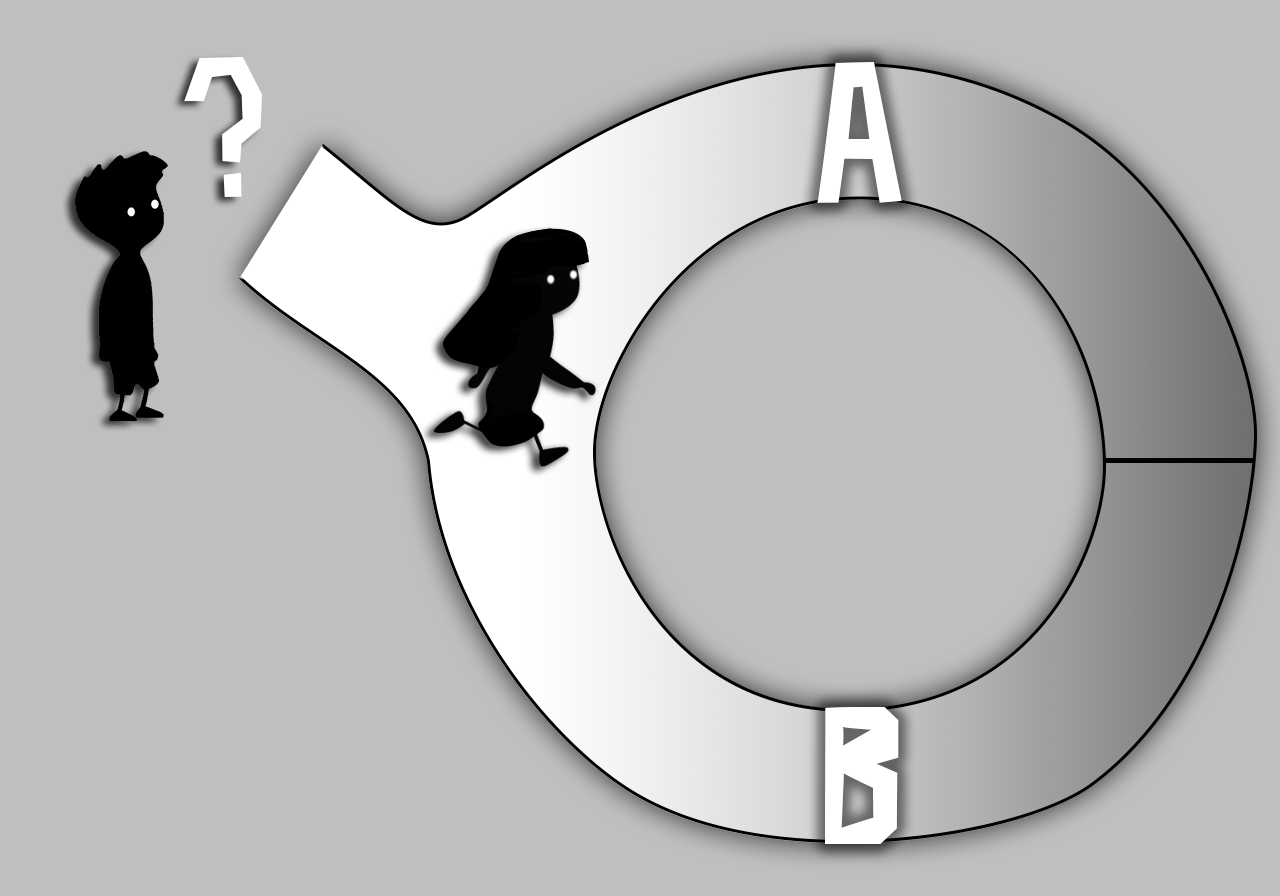
\includegraphics[width=1.\linewidth]{gfx/graficoJL_ZKP_1}\\The cave \citep{ZKPcave:fig}
		. Peggy takes randomly A or B. Victor awaits outside.}
	Peggy and Victor meet at the entrance of the cave, then Victor awaits while Peggy goes inside the cave, taking one of the passages, that we will name A and B. Victor can't see which way Peggy went. 
	
	When Peggy arrives at the door, \textbf{V}ictor enters the cave, and when he arrive to the fork, stops and yells which path, A or B, he wants Peggy to come back, to \textbf{v}erify she knows how to open the door.
	
	If Peggy actually knows the secret, she always can take the requested path, opening the magic door if needed.
	\marginpar{
\includegraphics[width=1.\linewidth]{gfx/graficoJL_ZKP_2}\\The cave. Victor chooses randomly the returning path for Peggy.}
	But if Peggy doesn't know the magic word, she had a chance of $50\%$ to guess correctly what passage Victor was going to ask. That means she had a chance to fool Victor.
	
	Victor then asks to repeat the experiment. With $20$ repetitions, the chances Peggy fools Victor in all of them is only  $2^{-20}$,
	\marginpar{
\includegraphics[width=1.\linewidth]{gfx/graficoJL_ZKP_3}\\The cave. Peggy returns by the requested path.}
	
	\textbf{E}ve, curious about what Victor and Peggy were doing in the cave, \textbf{e}avesdrops Victor during the process. The problem is that Eve doesn't know if Peggy and Victor agreed on what paths to choose, because they wanted to prank her for being busybody. Only Victor is confident he is choosing the returning passage randomly.
	
	Later, Victor is convinced that the door can be opened and Peggy knows the word, but he can't prove it to Eve because he can't open the door. 
\end{quote}





Based on ZKP properties, IBM has developed the Identity Mixer\footnote{Identity Mixer - \url{https://www.research.ibm.com/labs/zurich/idemix/}}, Idemix for short, protocol suite for privacy-preserving authentication and transfer of certified attributes. It allows user authentication without divulging any personal data. Users have a personal certificate with multiple attributes, but they can choose how many to disclose, or only give a proof of them, like being older than 18 years-old, living in a country without revealing the city, etc. Thus, no personal data is collected that needs to be protected, managed, and treated.

\begin{center}
	\textit{``If your personal data is never collected, it cannot be stolen.''}
\end{center}

%%%
So far, Idemix or privacy-ABCs have been successfully applied to deal with traditional Internet scenarios, in which users can authenticate and prove their attributes against Service provider. However, due to the reduced computational capabilities of certain IoT devices, it has not been yet considered for IoT scenarios. As we study in the state of the art chapter, current implementations are based on Java, which requires high computational and memory resources to be executed, and to the best of our knowledge, this is the first proposal that tries to apply an IoT solution for privacy-preserving authentication and authorization, based on Anonymous credential Systems, like Idemix.
%%5


As part of IBM's academic grant for \textit{Privacy Preserving Identity Management applied to IoT}, the goal of this project is to integrate Idemix with the IoT. It will be done using ABC4Trust's \acf{P2ABCE}, a framework that defines a common architecture, policy language and data artifacts for an attribute based ecosystem, cryptographically based on either IBM's Idemix or Microsoft's U-Prove \footnote{P2ABCEngine \url{https://github.com/p2abcengine/p2abcengine}}. This gives us a standardized language to exchange Idemix's messages between IoT devices and any other P2ABCE actor.

Once the IoT devices can execute Idemix, the new step is to take advantage of it in other deployments. In a smart building, different privacy policies could protect sensitive data, like how many people there are, and their identities, where a thermostat would only need to know if the amount of people is between some boundaries, but in case of emergency, the police department could request all the information available. We think that the first approach to achieve these ideas is first to integrate Idemix in known IoT identity systems, like FIWARE project. 

\hfil


\section{Outline of this thesis}

This document is structured as follows: In \autoref{ch:stateoftheart} we show a state of the art analysis through the history of Idemix and related works, analysing what is of the most interest for the IoT perspective; then, in \autoref{ch:objectives} we outline the project's objectives and analyse in depth the existing solutions that we are going to deal with; in \autoref{ch:design} we describe the formal design of the IoT and Idemix solution, and describe the PoC implementation developed; after an implementation, it is a must to validate it, as showed during the performance tests in \autoref{ch:validation}; finally, our conclusions and lines for future work are described in \autoref{ch:conclusions}.


\cleardoublepage
%\ctparttext{You can put some informational part preamble text here. 
%Illo principalmente su nos. Non message \emph{occidental} angloromanic
%da. Debitas effortio simplificate sia se, auxiliar summarios da que,
%se avantiate publicationes via. Pan in terra summarios, capital
%interlingua se que. Al via multo esser specimen, campo responder que
%da. Le usate medical addresses pro, europa origine sanctificate nos se.}
%\part{The Showcase}
%*****************************************
\chapter{State of the art}\label{ch:stateoftheart}
%*****************************************

In this chapter we present the two domains of this project: the Zero-Knowledge Proof based systems and the Internet of Things.


\section{Anonymous Credentials Systems}
% ZKP vs minimal disclosure como OAuth
% Persiano
% U -Prove
% Idemix
% P2ABCE 
% TODO: explicar P2ABCE
%\ac{P2ABCE}
% Credential: a certified container of attributes where an attribute has a type and a value

%%%
Other solutions are based on minimal disclosure. Standards like OAuth offer secure delegated access to the user information and when registering to a new service, the user can give a key to access only the data they want from another trusted service. This lets the service provider to work with the OAuth server, offering the same service as before without knowing as much data.

But this is only minimizes how many services have our data. Our OAuth provider could be attacked, revealing all our data, or our service provider, revealing now less data.
%%%

%%%%

A Quick Introduction to
Anonymous Credentials
Gregory Neven
IBM Zürich Research Laboratory
August 2008


Intuitively, an anonymous credential can be thought of as a digital signature by the Issuer on a list of
attribute-value pairs, e.g. the list
(fname=”Alice”, lname=”Anderson”, bdate=”1977/05/10”, nation=”DE”).
The most straightforward way for the User to convince a Verifier of her list of attributes would be to
simply transmit her credential to the Verifier. This approach has a number of disadvantages, most
notably
· that the User has to reveal all of her attributes so that the Verifier can check the signature;
· that the Verifier can reuse the credential to impersonate Alice wrt other Verifiers.
With anonymous credentials, the User never transmits the credential itself, but rather uses it to convince
the Verifier that her attributes satisfy certain properties – without leaking anything about the credential
other than the shown properties. This has the obvious advantage that the Verifier can no longer reuse the
credential to impersonate Alice. Another advantage is that anonymous credentials allow the User to
reveal a selected subset of her attributes. In the example above, Alice could for example reveal her first
name and last name, but keep her birth date hidden.
Stronger even, apart from showing the exact value of an attribute, the User can even convince the
Verifier that some complex predicate over the attributes holds. In particular, she can demonstrate any
predicate consisting of the following operations:
· Integer arithmetic: att+c , att+att , att·c : sum of attributes and/or constants, product of
attributes with constants
· Comparative: exp1 = exp2 , exp1 < exp2 , exp1 > exp2 , exp1  exp2 , exp1  exp2 : compare
arithmetic expressions over attributes/constants
· Logical: pred1 AND pred2 , pred1 OR pred2
Note that revealing a subset of attributes comes down to the special of showing that the predicate
att1 = val1 AND att2 = val2 AND …
holds. In the example above, Alice could show that she’s an overage national of an EU country by
showing that he has a credential satisfying
bdate  today – 18y AND ( nation=”DE” OR nation=”FR” OR … ) .
The Show protocol does not leak any information other than the truth of the statement. So in the
example above, not only does Alice’s name remain hidden from the Verifier, but so do her exact birth
date and nationality; the only information leaked is that her birth date is more than 18 years ago, and that
her nationality is one of the EU countries.
%%%

%%%%%%%%%%%%%%%%%%%%%%%%

@book{book:185217,
	title =     {Financial Cryptography: 8th International Conference, FC 2004, Key West, FL, USA, February 9-12, 2004. Revised Papers},
	author =    {Jack R. Selby (auth.), Ari Juels (eds.)},
	publisher = {Springer-Verlag Berlin Heidelberg},
	isbn =      {3540224203,9783540224204,9783540278092},
	year =      {2004},
	series =    {Lecture Notes in Computer Science 3110},
	edition =   {1},
	volume =    {},
	pages = {196-211},
	url =       {http://gen.lib.rus.ec/book/index.php?md5=24CD58AE88D5564A03C2E44B96732298}}


Persiano and Visconti presented a non-transferable anonymous
credential system that is multi-show and for which it is possible to prove
properties (encoded by a linear Boolean formula) of the credentials. Unfortunately,
their proof system is not efficient since the step in which a user proves
possession of credentials (that needs a number of modular exponentiations that
is linear in the number of credentials) must be repeated times (where is the
security parameter) in order to obtain a satisfying soundness

%%%%%%%%%%%%%%%%%%%%%%%%%


%%%%%%%%%
@book{book:947508,
	title =     {Security and Privacy in Communication Networks: 7th International ICST Conference, SecureComm 2011, London, UK, September 7-9, 2011, Revised Selected Papers},
	author =    {Zhiyun Qian, Z. Morley Mao, Ammar Rayes, David Jaffe (auth.), Muttukrishnan Rajarajan, Fred Piper, Haining Wang, George Kesidis (eds.)},
	publisher = {Springer-Verlag Berlin Heidelberg},
	isbn =      {978-3-642-31908-2,978-3-642-31909-9},
	year =      {2012},
	series =    {Lecture Notes of the Institute for Computer Sciences, Social Informatics and Telecommunications Engineering 96},
	edition =   {1},
	volume =    {},
	pages = {243-260},
	url =       {http://gen.lib.rus.ec/book/index.php?md5=A7667DB3EE5B36AAA6E93AE07E888D8D}}

U-Prove. Stefan Brands provided the first integral description of the U-Prove
technology in his thesis [6] in 2000, after which he founded the company Credentica
in 2002 to implement and sell this technology. Microsoft acquired Credentica
in 2008 and published the U-Prove protocol specification [5] in 2010
under the Open Specification Promise4 together with open source reference software
development kits (SDKs) in C# and Java.
The U-Prove technology is centred around a so-called U-Prove token. This
token serves as a pseudonym for the prover. It contains a number of attributes
which can be selectively disclosed to a verifier. Hence the prover decides which
attributes to show and which to withhold (e.g. one can reveal the birth date,
but not the residence address). Besides the attributes the token contains two
information fields, one defined by the issuer, and one by the prover. These fields
are always disclosed and can be used to provide some meta data such as a validity
date of the token. Finally there is the token’s public-key, which aggregates all
information in the token, and a signature from the issuer over this public-key to
ensure the authenticity

5. Brands, S., Paquin, C.: U-Prove cryptographic specification v1.0. Tech. rep., Microsoft
Corporation (March 2010)
6. Brands, S.A.: Rethinking Public Key Infrastructures and Digital Certificates:
Building in Privacy. MIT Press (August 2000)
%%%%%%%%%%%





%% Idemix:

En \citep{Camenisch:GroupSig} \citep{Camenisch:AnonCred} \citep{camenisch2002signature} describen los métodos criptográficos iniciales utilizando ZKPs que evolucionarán a Idemix. En \citep{idemixSpec} se encuentra la especificación actual del protocolo Identity Mixer de IBM.

\section{Internet of Things}

% Adaptar seguridad "clásica" de cifrado de mensajes con claves simétrica y asimétrica, RSA, curva elíptica, DH, 
% Que el principio de las ZKP ya se usaba en las tarjetas, de manera básica, pero no como parte de un sistema mayor como Idemix
% Vanets y otros intentos de meter sistemas previos en IoT

Regarding the Internet of Things security, 


\section{Idemix}

\paragraph{TODO: Move to motivation}

%%%%
The problem of Internet security has been approached by securing the transmission channel (e.g. SSL/TLS) and the data stored in both ends (strict access policies, local encryption, etc.). In the end, the data exists in two entities, the owner of the data and the service provider. The owner is the most interested in securing his data, and can apply as many measures as he wants, but only on his side of the table. The service provider that stores the user data needs it to provide the service, and a successful attack would reveal many users data, aside from how many measures each one used to protect it. The case of PlayStation Network outage in 2011 \citep{PSN2011} affected 77 million accounts, with suspected credit card fraud, is an example of this kind of attacks.

\hfil

%%%%


%%%%%%%%%%%%%%

Estudio teórico de cómo integrar Idemix en una smart card, según el reparto de cálculos y valores secretos \citep{luuk}.
Implementación de Idemix en smart cards MULTOS \citep{vullers2013efficient}
\citep{sucasas} Diseño de sistema anonymous credential system with sc support, y haciendo pruebas en simulador de smart card, sin embargo no utilizan Idemix ni dan toda su funcionalidad, pero sí aportan un estudio de cómo afrontar la implementación: smart cards.
Integración en IoT device con P2ABCE en \citep{vanet}





Why ABC4Trust Card Lite: soporte de las APDUs del proyecto P2ABCE, más grande, multi-engine, como dice su powerpoint, adaptable a cualquiera que use Discrete Log.Objectives
%\addtocontents{toc}{\protect\clearpage} % <--- just debug stuff, ignore
%************************************************
\chapter{Analysis and objectives}\label{ch:objectives}
%************************************************

% descripción del proyecto: objetivos, metodología: pasos del diseño y desarrollo, ver figura 3.1 (elección de sensores: computing offloading), contexto (partimos de ABC4T: recordar P2ABCE y que se basa en tarjetas), entorno de desarrollo (meter elección del Omega2, LEDE, teoría de APDUs, código heredado) el sw, los tests p2abce puro, 


%TODO resumir organización del capítulo
% Incluir bibliografía: vanet, wiki


In this chapter we describe the project objectives, and the methodology followed during its development. In section ... TODO

\section{Project description}

The purpose of this project is the integration of IBM's privacy preserving solution, Idemix, in the environment of the Internet of Things. The objective is to design a general solution for the existing IoT devices and systems, without compromising any feature of Idemix, and provide a working PoC in a real IoT environment, even though it isn't the most constrained scenario. The project is aimed to be used in privacy-preserving environments, providing security for IoT, controlling what data is being disclosed and to whom.

In a smart city project, citizens' data can be privatized and at the same time continue to offer the benefits of the sensors around. Authorized personnel can disclose the information when required, like fire-fighters accessing a building's sensors to check how many people there are and what conditions they are in, in case of an emergency; but keep such invasive data private to other non-critical services, for example, only giving a proof that there are people in a floor of the building, to activate or deactivate the air-conditioning system.

\hfil

% TODO: numerar objetivos: nombrarlos luego por el número cuando se consiguen, empiezan, en conclusiones...
% TODO: no tan obvio que se han definido objetivos tras el proyecto.

We will divide the project in various \textbf{objectives}, starting from the principal goal, dividing our work in different categories.

\hfil

\paragraph{Idemix and the IoT}
This is our main objective, integrating IBM's privacy-preserving system in the IoT environment. 

\paragraph{Analysis} Study the state of the art of Idemix and the IoT, analysing related projects, papers with similar approaches, and consider the best fitting solutions from where to begin.

\paragraph{Design and implementation} After studying the existing works, we must give a formal solution to be implemented. This includes the theoretical architecture, the steps to take, the software to implement, the hardware to use, and any simplifications to leave as future work.

Our \textbf{software} objectives include making it easily maintainable, structured and extensible, from the IoT and original project perspectives, that is, the IoT solution must be interoperable with other non-IoT solutions, now and in the future, with minimal effort, given new IoT systems or changes in the cryptographic protocols.

Our \textbf{hardware} objective is to use devices as constrained as possible. But considering our early situation in the project, we will use IoT devices that ease testing and development, having in mind the other devices, and what specific steps we should take for them in the future.

\paragraph{Validity and evaluation} Deploy a \ac{PoC} in a \textbf{real scenario}, without the need of simulators, checking it works as expected, and measuring its performance.



\section{Methodology}

Giving the vast range of IoT devices, a one-for-all solution must take in consideration multiple requirements and limitations. We will break down the original system, Idemix and P2ABCE, analyze every part of it and categorize them. We will consider what components are mandatory to be executed in the target device that wants to act as User of Verifier, and which components the devices would actually be able to execute.

Devices with equivalent processing power to smart phones are capable of running the current Java implementations of P2ABCE with Idemix, but the most constrained IoT devices can not handle the entire system, only the mandatory cryptographic operations.

Using the technique known as \textit{Computation Offloading} we can design an IoT architecture where the most constrained targets can keep their private keys and certificates secure within the device, and act as any other actor in the P2ABCE system. Studying the original P2ABCE architecture and implementations we will identify the key operations to be executed in the constrained device, and how to communicate efficiently during the delegation.

After the technical design, we will implement the PoC, using known software designs patterns, that will improve the maintainability of the project. Taking advantage of this practices, we can document the immediate steps for future developers, how to reimplement certain interfaces when porting the application to a new system, or where the core logic lies, to implement future protocol changes.

Finally, the PoC will be evaluated to assert that we achieved our goals, and measure its performance, judging if it can indeed be suitable for a IoT deployment.



\section{Analysis of P2ABCE}

There are several cryptographic systems for dealing with attribute-based
identities. Typically these systems distinguish credentials and attributes. Informally,
a credential is a cryptographic container of attributes, where an attribute has a type and a value \citep{vullers2013efficient}.

\begin{figure}[bth]
	\begin{center}
		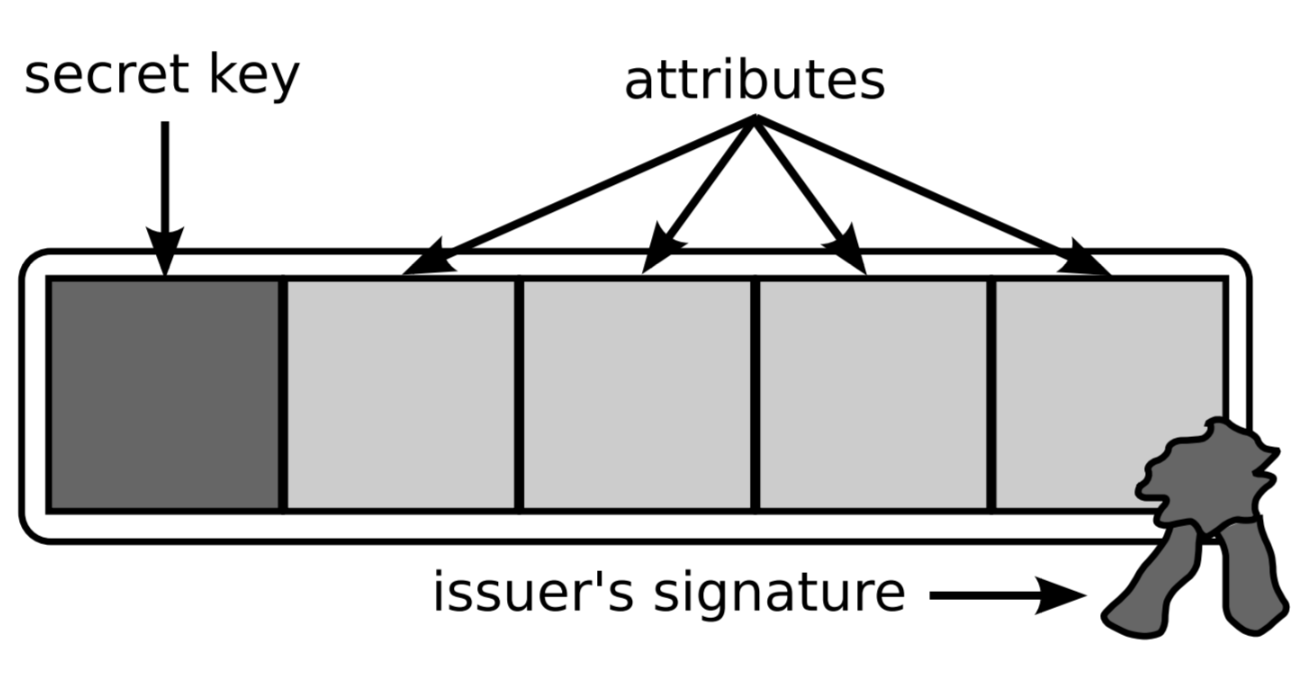
\includegraphics[width=0.4\linewidth]{gfx/ABC}
	\end{center}
	\caption{A first look at an attribute-based credential with four attributes.}
	\label{fig:abc}
\end{figure}



The Privacy Preserving Attribute Based Credentials system is composed by several actors, each one of them with different roles. One entity could act with more than one role, e.g., in a M2M (Machine To Machine) scenario, a device could act as both User and Verifier to other peers; but one can assume each actor acts with one role at a time.


The roles are:


\begin{figure}[bth]
	\begin{center}
		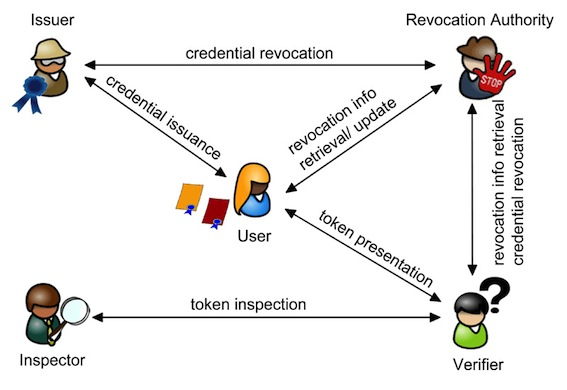
\includegraphics[width=\linewidth]{gfx/actors}
	\end{center}
	\caption{Entities in a P2ABC System}
	\label{fig:actors}
\end{figure}

\begin{itemize}
	\item \textbf{Issuer}\\
	In the ABC infrastructure, the Issuer is a trusted entity responsible for issuing credentials, vouching for the correctness of the information contained. Each Issuer generates a secret key and publishes the Issuer parameters that include the corresponding public verification key.
	
	\item \textbf{User}\\
	Entities that collect credentials from various Issuers. They can decide between all their credentials which attributes and values to present when making assertions about their identity to service providers.
	
	\item \textbf{Verifier}\\
	A service provider that protects access to a resource by imposing restrictions on the credentials that users must own and the information from these credentials that users must present in order to access the service.
	
	\item \textbf{Revocation Authority} (optional)\\
	This entity is responsible for revoking issued credential, preventing their further usage to generate a presentation token. Each revocation authority generates and publishes its revocation parameters.
	
	\item \textbf{Inspector} (optional)\\
	The Inspector's duty is to de-anonymize the user's presentation token under specific circumstances (e.g. misuse or liability). At setup, each inspector generates a private decryption key and a corresponding public encryption key. Usually, the capability of inspection should be bonded to privacy protection laws.
	
\end{itemize}


The cryptographic nature of the credential-as-container concept includes the
following four security aspects \citep{vullers2013efficient}:
\begin{itemize}
	\item The issuer’s digital signature ensures \textbf{authenticity}: the credential originates
	from the issuer, and this issuer asserts that the attributes hold for the person.
	\item This signature also guarantees integrity: the attributes contained in the credential
	have not been altered since they were issued.
	\item A credential is \textbf{non-transferable} as it is bound to the secret key, only known by the credential owner.
	\item A credential \textbf{hides} its content, so it does not reveal the attributes it contains.
	Furthermore, a credential protects the privacy of its owner through the following
	cryptographic properties.
	\item Issuer \textbf{unlinkability} ensures that any information gathered during issuing
	cannot be used to link a verification of the credential to its issuance.
	\item \textbf{Multi-show unlinkability} guarantees that when a credential is verified multiple
	times, these sessions cannot be linked.
\end{itemize}

Zero-knowledge proofs, used in Idemix, allow a user to prove ownership of a credential without
revealing the credential itself. Since the verifier does not see the credential, verification
instances are unlinkable and they also cannot be related to the issuing procedure. The privacy of users is protected by these unlinkability properties, even if the credential issuer and all verifiers collude.



To sum up, an attribute-based credential contains attribute-value pairs that are certified by a trusted Issuer. A credential can also specify one or more Revocation Authorities who are able to revoke the credential if necessary. Using her credentials, a User can form a presentation token that contains a subset of the certified attributes, provided that the corresponding credentials have not been revoked. Additionally, some of the attributes can be encoded in the presentation token so that they can only be retrieved by an Inspector. Receiving a presentation token from a User, a Verifier checks whether the presentation token is valid w.r.t. the relevant Issuers and Inspector's public keys and the latest revocation information. If the verification succeeds, the Verifier will be convinced that the attributes contained in the presentation token are vouched by the corresponding Issuers.


\hfil

In the P2ABCE repository \citep{p2abcurl} there is available the project's code, divided in two solutions: a complete P2ABCE implementation in Java and a MULTOS smart card implementation as PoC for the project.

\subsection{P2ABCE Code Structure and REST Services}

The Java code is managed by a Maven project, structured using various known design patterns, but not of our interest. The part we are actually interested in are the \textit{REST Services} and their use of the \textit{Components} classes, where the smart card's logic and use are defined.

P2ABCE project is based on the concept of smart cards, virtual or physical, to store the credentials. An interface is defined to communicate with these smart cards, and then different implementations allow to use either \textit{Software Smartcards} or \textit{Hardware Smartcards}. 

The \textit{SoftwareSmartcard} class implements the interface in Java, suitable for applications using P2ABCE self-storing digital smart cards, like a virtual wallet.

The \textit{HardwareSmartcard} class uses the standard APDU messages (\ref{subsec:APDU}) to interact with smartcards. P2ABCE defines the necessary APDU instructions for the smart card needed to implement each method of the interface. It relies on \textit{javax.smartcardio} abstract classes (implemented by Oracle in their JRE) to communicate the smart card reader and the smart card. This way, it doesn't matter what manufacturer issues the smartcard, or if it's an Android device with NFC, if they support the APDU instructions, P2ABCE will work with them.

\begin{figure}[bth]
	\begin{center}
		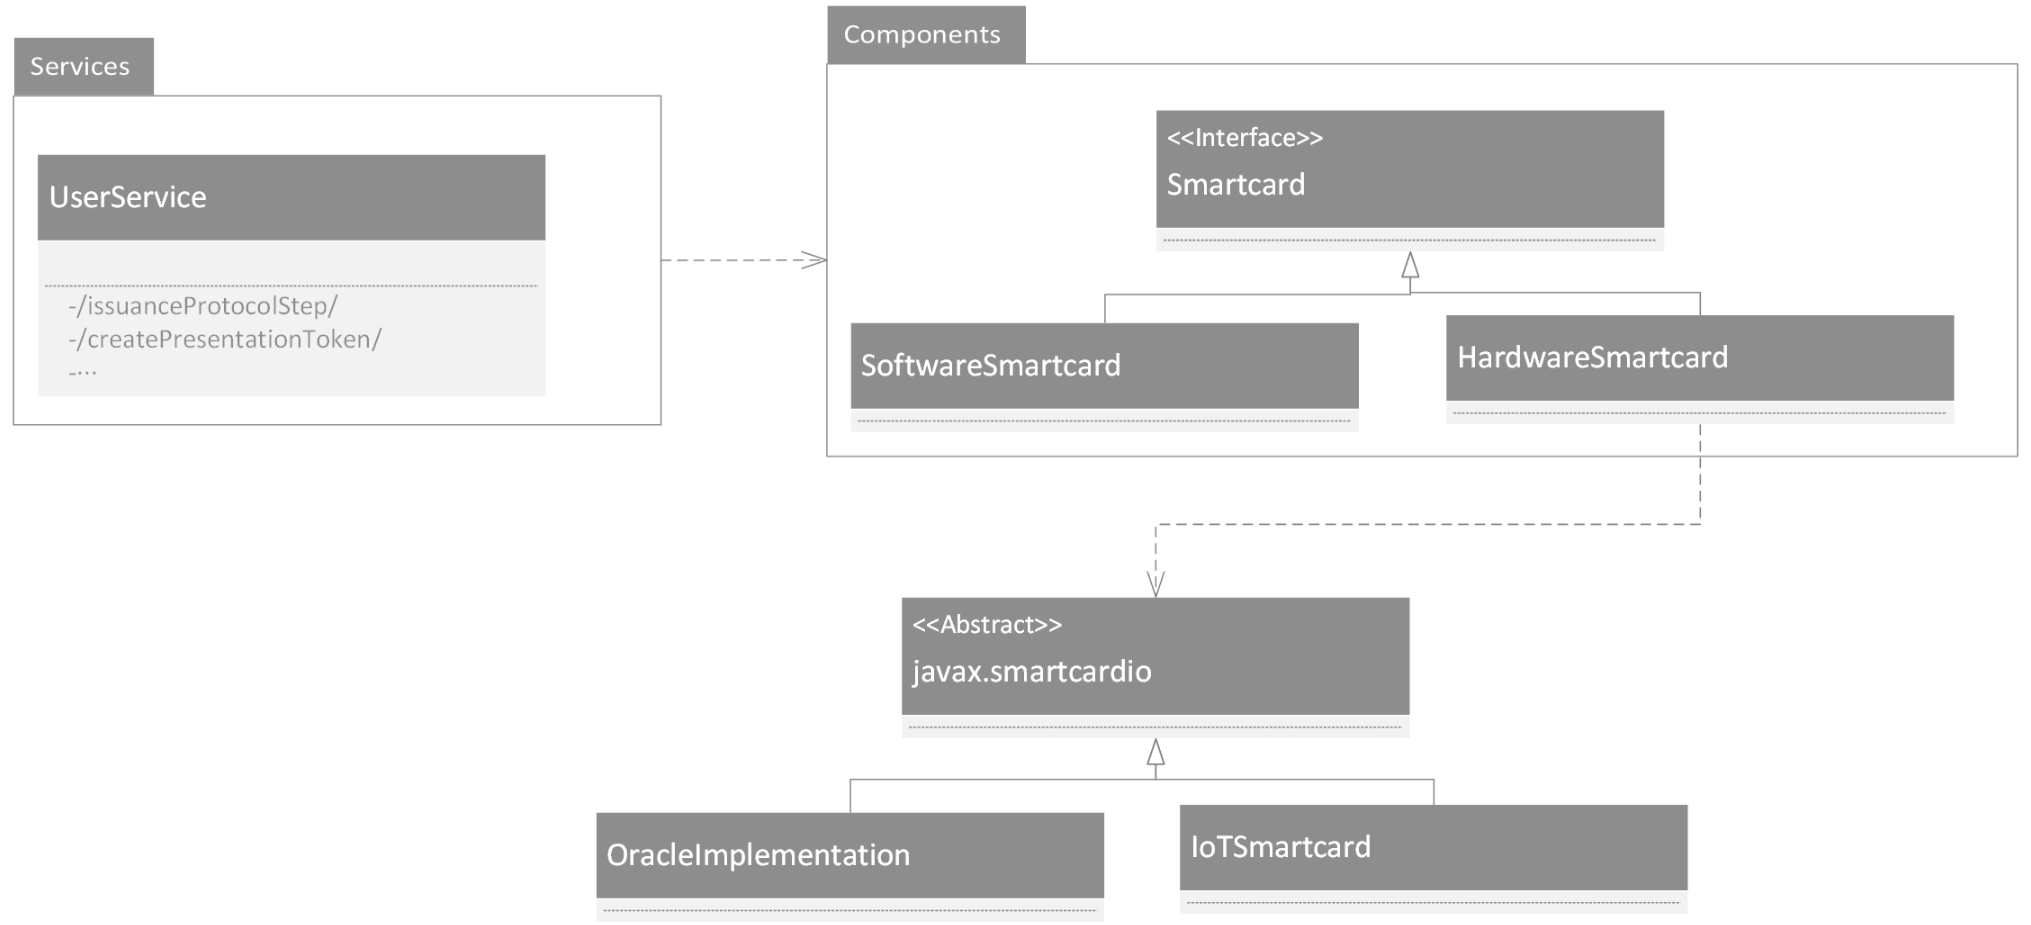
\includegraphics[width=\linewidth]{gfx/p2abceBasicUML}
	\end{center}
	\caption{Basic P2ABCE structure}
	\label{fig:p2abceBasicUML}
\end{figure}


\hfil

The project also provides a set of REST services to control each role of the P2ABCE systeam (User, Issuer, Verifier, Inspector, etc.). The methods implemented include the creation of \textit{Software} smart cards within the User Service, and store them in a data base for future REST calls that may need them.

The services receive parameters like the length of the cryptographic keys, IDs, or XML files to parse. The REST API is not meant for a User Service to communicate with an Issuer Service, for example, but for the User actor to call the Engine through the User Service, to perform specific actions, and then the Service returns the response XML. Those XML files are the way to communicate two different actors. The transmission method to exchange the XML depends on the specific scenario.



\subsection{ABC4Trust Card Lite}

As a PoC the P2ABCE project includes a smart card reference implementation, the ABC4Trust Card Lite \citep{ABC4TCardLite}. It supports device-bound U-Prove and Idemix, and virtually any discrete logarithm based pABC system.

Version 1.2 is written for \texttt{ML3-36K-R1} MULTOS smart cards, with approximately 64KB of EEPROM (non-volatile memory), 1KB of RAM and an Infineon SLE 78 microcontroller, a 16-bit based CPU aimed for chip cards.

The card stores the user's private key $x$ and any \ac{BLOB} that the P2ABCE may need (like user's credentials). Then P2ABCE delegates the cryptographic operations on the smart card, that operates with $x$.

\begin{figure}[bth]
	\begin{center}
		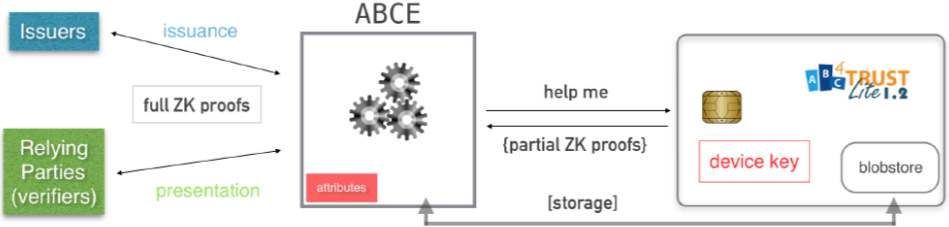
\includegraphics[width=\linewidth]{gfx/ABC4TCardLite}
	\end{center}
	\caption{ABC4Trust Card Lite}
	\label{fig:ABC4TCardLite}
\end{figure}

The cryptographic operations performed by the smartcard are the modular exponentiation and addition used by ZKPs based on the discrete logarithm problem.

\hfil

The code is available from the P2ABCE's repository and has some good and bad points to have in count:

The best asset of this code is that it's written in C aiming to a very constrained device, with very limited memory and similar computational power to many other IoT devices.

The code uses some good practices when programming for constrained devices, also explained in the first implementation of Idemix in smart cards \citep{vullers2013efficient}. Aside the implementation in assembly code of some operations to accelerate the execution, most techniques aim to reduce the memory usage. They define \texttt{union} data types to join variables never used at the same time, so they can be stored on the same data location. Instead of function parameters, most variables are made global, reducing the space on the stack used when calling other functions. If parameters are needed, they are pointers to shared buffers with fixed sizes, avoiding the use of any dynamic memory allocation.


Although, among the many drawbacks, we could highlight the \textit{awful} coding style, the strong dependency on MULTOS framework and many bugs found. 

The code is structured in two files, \textit{main.h} and \textit{main.c}, with around $550$ and $5200$ lines of code, respectively.

The file \textit{main.h} is mostly a reimplementation in assembly MEL code of some MULTOS functionality already offered by their API.

The \textit{main.c} consists on nearly $600$ lines of variables and data structures declarations; followed by the \textit{main()} function, a $2600$ lines long \textit{switch-case} expression, with practically no comments; and to conclude, the implementation of thirty functions called \textit{Subroutines} at the end of the file, around other $2000$ lines of code.

\hfil

At this stage, we have two options to implement our IoT device compatible with P2ABCE:

\begin{itemize}
	\item Implement in C the \textit{Smartcard} interface used by P2ABCE architecture, and use some communication protocol to remotelly call the methods from the machine running the P2ABC Engine.
	\item Present the IoT device as a hardware smart card, using the APDU protocol (already defined, standard and with minimal overload). Providing a \textit{javax.smartcardio} ``IoT implementation'' to communicate with the IoT device through a transmission protocol, making the already existing \textit{HardwareSmartcard} class compatible with the new \textit{IoTSmartcard} running in the IoT device.
\end{itemize}

Even with the problematic to maintain or even understand the code of ABC4Trust Card Lite, once one studies MULTOS framework in deep and applies many refactoring techniques to the code, it becomes the best starting point for the IoT version, making us opt for the second option.





\section{Preliminaries about smart cards}

In this section we will introduce a brief description of the APDU standard protocol, and the MULTOS framework used by the ABC4Trust Card Lite.


\subsection{Smart Card Communication Protocol}\label{subsec:APDU}

To communicate the smart cards and the reader the \texttt{ISO/IEC 7816-4} \citep{APDUISO} specifies a standardized protocol .

The messages, also kown as \acp{APDU}, are divided in APDU Commands and APDU Responses.

\textbf{APDU Commands} consist in 4 mandatory bytes (CLA, INS, P1, P2), and an optional payload.

\begin{itemize}
	\item CLA byte: Instruction class. Denotes if the command is interindustry standard or proprietary.
	\item INS byte: Instruction code. Indicates the specific command.
	\item P1, P2 bytes: Instruction parameters.
	\item Lc, 0-3 bytes: Command data length.
	\item Command data: Lc bytes of data.
	\item Le, 0-3 bytes: Expected response data length.
\end{itemize}

This way, minimal number of bytes are needed to transmit commands to the smart card, allowing manufacturer's personalization of the smart card behavior and capabilities along with standard operations.

\begin{figure}[bth]
	\begin{center}
		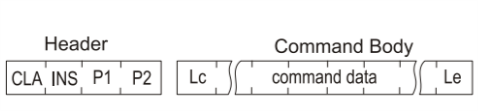
\includegraphics[width=0.55\linewidth]{gfx/APDUCommand}
	\end{center}
	\caption{APDU Command}
	\label{fig:APDUCommand}
\end{figure}


\textbf{APDU Responses} are generated inside the smart card, always as an answer to an APDU Command. They consist on an optional payload and two mandatory status bytes.


\begin{itemize}
	\item Response data: At most Le bytes of data.
	\item SW1-SW2 bytes: Status bytes. Encode the exit status of the instruction.
\end{itemize}

\begin{figure}[bth]
	\begin{center}
		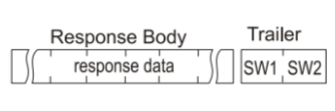
\includegraphics[width=0.55\linewidth]{gfx/APDUResponse}
	\end{center}
	\caption{APDU Response}
	\label{fig:APDUResponse}
\end{figure}




\hfil


The transmission protocol varies between different types of readers and smart cards (e.g. chip, contact-less), but what is common between every smart card interaction, is the \textit{APDU Command-Response Dialogue}. As long as the smart card has a power supply, it can maintain the memory in RAM between APDU Commands, what allows to do in two or more steps complex operations, transmit more bytes than a single APDU can admit, etc.

\hfil




\begin{figure}[bth]
	\begin{center}
		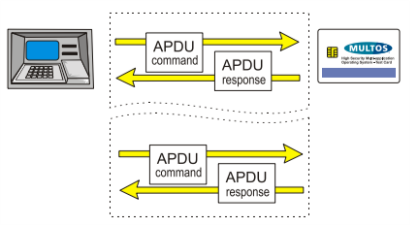
\includegraphics[width=0.75\linewidth]{gfx/APDUdialog}
	\end{center}
	\caption{APDU Command-Response Dialogue}
	\label{fig:APDUdialog}
\end{figure}

Originally, the Lc and Le bytes had only 1 byte, if present, restricting the payload data to be at most 256 bytes long. An extension to the protocol changed the meaning of a Lc or Le 0x00 byte (256 bytes long payload), so when the byte corresponding to Lc or Le started with 0x00, the next two bytes where the real length.  With this, an Extended APDU lets up to $65536$ bytes of data.

The problem here, is that not all readers or smart cards support extended APDUs. Originally, to send more than 256 bytes of data in an APDU Command, a \textit{Put Data} instruction is defined, so the smart card stores the payload in a buffer, until other APDU Command indicates how to use it.

To send more data in an APDU Response, the status bytes are set to: SW1=0x61 and SW2 to the remaining bytes to send. Because a smart card can't send APDU Commands, the card terminal must send a \textit{GET RESPONSE}, a special APDU Command, with Le set to the number of bytes specified in SW2. Iterating this process, the smart card can send as many bytes as it wants as Response.

With the introduction of Extended APDUs, this technique is no longer needed.






\subsection{MULTOS}

MULTOS is a multi-application smart card operative system, which provides a custom developing environment, with rich documentation \citep{MultosTechLib}. MULTOS smart cards communicate like any other smart card following the standard, but internally offers a very specific architecture, affecting the way one must code applications for it.

In this section we will present the main characteristics of a MULTOS smart card that shaped the ABC4Trust Card Lite code and that we had to be aware of when adapting it to IoT devices.


\paragraph{MULTOS programming languages} A native assembly language called MEL, C and, to a lesser extent, Java, are the available languages to code for MULTOS. In our case, ABC4T Card Lite uses MEL and C.

\paragraph{Execution Model}
Applications on a MULTOS card are executed in a virtual machine, called the Application Abstract Machine (AAM). The AAM is a stack machine that interprets instructions from the MULTOS Executable
Language (MEL).

The transmission and communication process is done by MULTOS core, and it then selects, based on the CLA byte of the APDU, the application to load. This application is what most developers will only worry about, and is where their compiled \texttt{main()} function will start.

\begin{figure}[bth]
	\begin{center}
		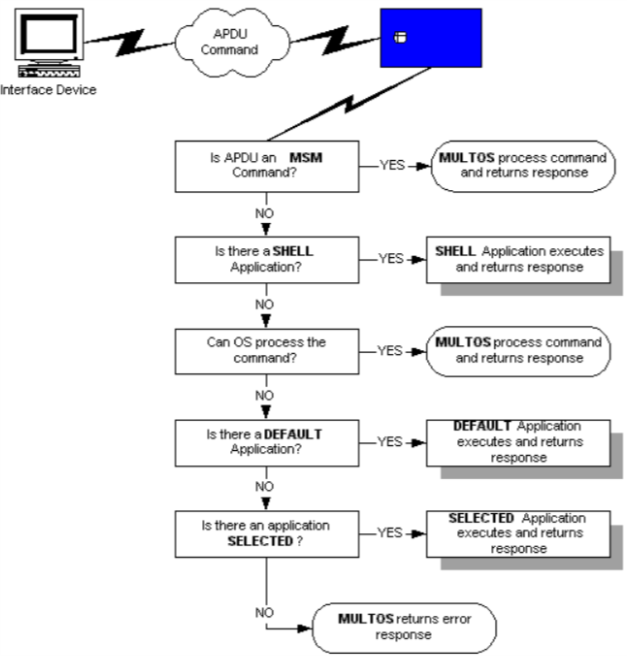
\includegraphics[width=0.6\linewidth]{gfx/multosWorkflow}
	\end{center}
	\caption{MULTOS Workflow}
	\label{fig:multosWorkflow}
\end{figure}

Now the developer is in charge of checking what instruction was sent, handle it with regard to his domain logic,  write in the specific data space the APDU Response bytes, and call \texttt{multosExit()}, a MULTOS API function that will be in charge to send the APDU Response.
In summary, our application starts with all data loaded in memory and exits without worrying how the answer is sent back.

As we can see, MULTOS is a comfortable framework to develop smart card applications, and now we must adapt and implement it for our IoT devices, if we want to port ABC4Trust Card Lite's code.



\paragraph{MULTOS Memory Layout}

Each application in MULTOS has access to a specific memory layout, divided in different categories:

\begin{figure}[bth]
	\begin{center}
		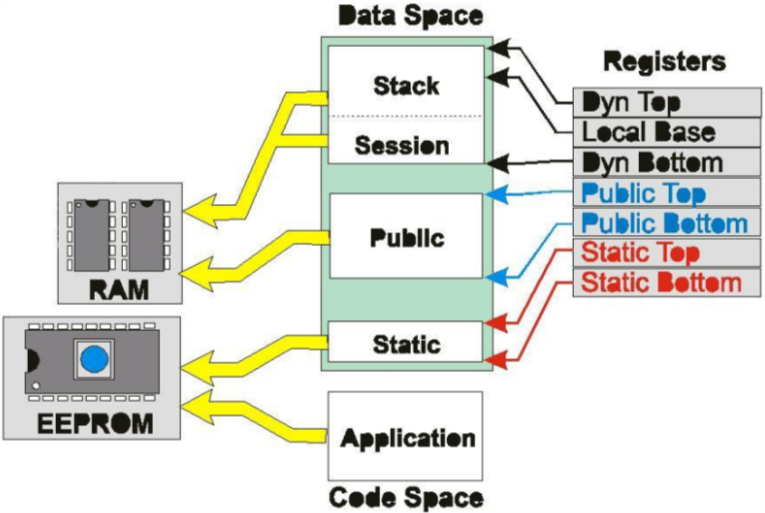
\includegraphics[width=0.8\linewidth]{gfx/multosMemLay}
	\end{center}
	\caption{MULTOS Memory Layout}
	\label{fig:multosMemLay}
\end{figure}


The Code Space is where the application code is stored.
The Data Space is divided in Static memory, Public memory and Dynamic memory.

\textbf{Static memory} are the application variables declared after the specific \textit{\#pragma melstatic} compiler directive. These variables are stored in the non-volatile secure EEPROM, and any write is assured to be saved because they are not loaded into RAM.

\textbf{Public memory} can be seen as the input/output buffer for applications and MULTOS system. The APDU header appears at the top of Public, and command data at the bottom. The application writes then the APDU Response bytes in Public, at specific position (see \autoref{fig:multosPubMem}). To declare variables in this data space, the \textit{\#pragma melpublic} directive is available.

\textbf{Dynamic memory} works like usual program memory, with Session Data storing global variables and the Stack. The limited size of RAM in IoT devices and smart cards makes the use of dynamic memory not advisable. The compiler directive to use Session Data is \textit{\#pragma melsession}.


\begin{figure}[bth]
	\begin{center}
		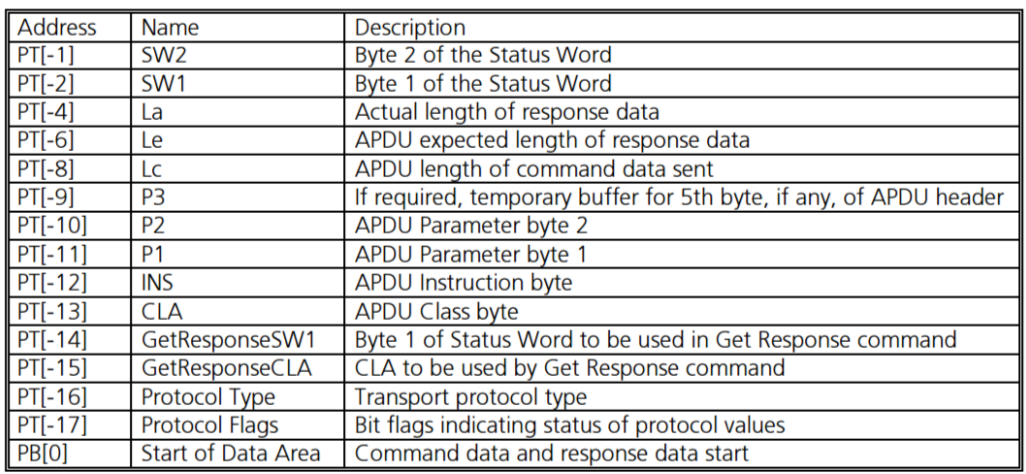
\includegraphics[width=\linewidth]{gfx/multosPubMem}
	\end{center}
	\caption{MULTOS Public Memory Data Map}
	\label{fig:multosPubMem}
\end{figure}


\hfil


With regards to primitive types, to avoid confusion with their sizes, MULTOS defines and uses the following data types specified in \autoref{fig:multosDataTypes}. It's important to notice that MULTOS is Big Endian
\marginpar{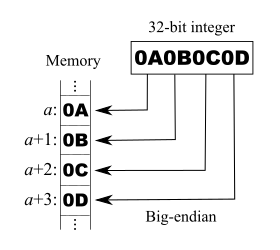
\includegraphics[width=\linewidth]{gfx/Big-Endian}\\Big-Endian, Wikipedia}
and when storing structures there is no padding between defined variables, unlike modern compilers that perform data structure alignment \citep{dataStructAlign} for performance.

\begin{figure}[bth]
	\begin{center}
		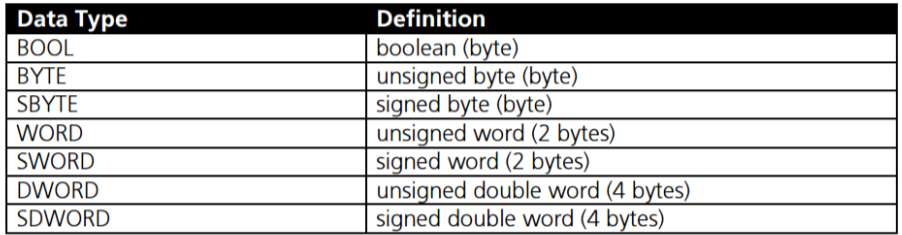
\includegraphics[width=\linewidth]{gfx/multosDataTypes}
	\end{center}
	\caption{MULTOS Data Types}
	\label{fig:multosDataTypes}
\end{figure}


\paragraph{MULTOS Standard C-API}

A collection of more than a hundred functions are provided for arithmetic, cryptography, memory and smart card operations. The \textit{multos.h} interface provides access to these functions, that ultimately call their respective primitive instructions in assembly code. The primitive instructions are but a system call with an operation code, loading data in the needed registers. Therefore,  no implementation for these tools is available, nor in C, nor in assembly code.

Nevertheless, the C-API documentation \citep{MultosTechLib} provides rich description for each function.




\hfil

\section{Development environment}


For almost every IoT device in the market, there exists a C compiler and many frameworks available to build firmware binaries, like Arduino Core, Contiki, Mongoose OS, ThreadX OS, OpenWrt, LEDE, proprietary SDKs, etc. Each firmware targets a specific range of devices, depending on processing power and memory limitations. For example, Arduino and Contiki aim for very constrained microcontrollers, like Atmel's ATmega or TI's MSP430, but can also be used in ESP8266, a more powerful device, with WiFi capabilities.
\marginpar{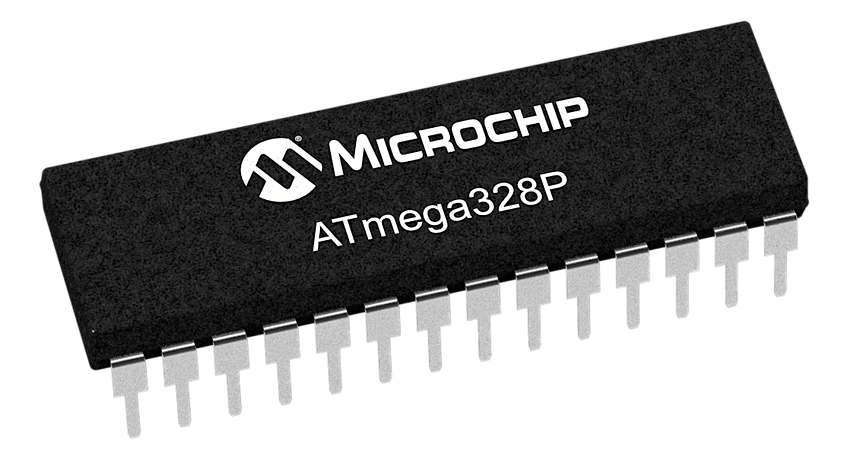
\includegraphics[width=0.8\linewidth]{gfx/ATmega328P}\\$ATmega328P$}

Starting a big project development for \ac{IoT}, aiming the most constrained devices may not be a good idea. The lack of usual OS tools, like POSIX, threads, or minimum I/O, like a terminal, can make debugging a tedious task. With good programming practices, one can start from the top and slowly end with more constrained devices and reliable code.


For this reason, the current \ac{PoC} is developed on LEDE, Linux Embedded Development Environment \citep{ledeproject}, using the Onion Omega2 development board. Although the Omega2 uses LEDE, its microcontroller is also listed as compatible with ThreadX OS \citep{THREADX}, a Real-Time Operative System for embedded devices, therefore, the performance measured in our PoC can be relevant to real scenarios with similar hardware.

The PoC will take advantage of the Linux system using mainly files and sockets like in any other Linux desktop distribution, so we can focus on the project itself rather than the specific platform APIs for storage and connectivity.


\hfil

The project development is divided between the IoT device code and the P2ABCE services. To ease the setup of new developing machines, we will use Docker to deploy containers ready to compile the code.

\hfil

P2ABCE is already written in Java and uses Maven to manage dependencies. The project needs some minor changes to work with our IoT architecture. Any text editor or Java IDE is suitable for the development, because the compilation is done through the terminal, with Maven commands.

We compile the project inside a Docker container, with OpenJDK 7, Maven 3 and Idemix 3.0.36, following the project \href{https://github.com/p2abcengine/p2abcengine/wiki/How-to-Build-the-ABC-Engine}{instructions} to use Idemix as the Engine for P2ABCE.

\hfil

We can assume all IoT devices have a C cross-compiler, some even a C++ cross-compiler. The worst case scenario is that one must write assembly code, and that code will be specific of that target, so we won't consider them.
If now we focus on the most constrained devices, we could find out that for some we can't use C++, some may not have many usual libraries, moreover, the memory limitations they face make practically impossible to use dynamic memory, if we want to avoid many execution malfunctions.

For that reason, the developed code for IoT devices should be written with standard C, without using dynamic memory or third party libraries.

\hfil


To manage the PoC code we chose CMake, providing many advantages over Makefiles:

\begin{itemize}
	\item Cross-platform. It works in many systems, and more specifically, in Linux it generates Makefiles.
	\item Simpler syntax. Adding a library, files to compile, set definitions, etc. can be done with one CMake command, with rich documentation on the project's \href{https://cmake.org/cmake/help/latest/}{website}.
	\item Cross-compilation. With only a \href{http://www.vtk.org/Wiki/CMake_Cross_Compiling#The_toolchain_file}{\small{CMAKE TOOLCHAIN}} file, CMake sets up automatically the cross-compilation with Makefiles and the C/C++ cross-compiler provided.
\end{itemize}


\hfil

Although the ideal final code is written in pure C, without external libraries or dynamic memory, the PoC uses three major libraries:

\begin{itemize}
	\item OpenSSL: Provides reliable and tested AES128, SHA256 and random number generator implementations.
	\item LibGMP: Provides multiprecision integer modular arithmetic.
	\item cJSON: Provides a JSON parser to store and read the status of the device, in a human readable way.
\end{itemize}

These three libraries are used to implement different interfaces in the project, and C implementations of these interfaces should replace the external libraries in the future.

\hfil

Finally, we use Docker to deploy the compilation environment. Our container includes CMake and the LEDE SDK \citep{ledeproject}, configured for the Omega2 target, the device chose for the PoC.

The Dockerfiles and CMake cross-compilation toolchain can be found in \autoref{ch:docker}.

%************************************************
\chapter{Design and implementation}\label{ch:design}
%************************************************

% Estructura:
% +Design
%  -Architecture design: delegation, computation offloading, duality User/SC + Engine
% 


In this chapter we will describe the process for defining how a constrained IoT device may be integrated in a system like P2ABCE. We will also describe the PoC implementation carried out to test a realistic deployment.

\section{Design}

In this section we will define how an IoT device may be integrated in the P2ABCE architecture, being totally compatible with any other system using P2ABCE, addressing the power and memory constrains many IoT devices face.

We decided to use P2ABCE with the Idemix as its Engine, because it is officially supported by the Idemix Library, it has the most up-to-date implementation, as we saw in the state of the art, and adds capabilities to Idemix like the Presentation Policies, or interoperability with U-Prove, not available without the P2ABCE project.

Our main goal is to make an IoT device capable to act as a User or Verifier in the P2ABCE architecture. For this, the device should be able to \textbf{communicate} with the Verifier or Prover with which it is interacting, manage the P2ABCE complex \textbf{XML schemas} transmitted, and perform the \textbf{cryptographic operations} required.

The communication between actors depends on each IoT scenario, it can be achieved with many existing standard solutions, e.g. an IP network, a Bluetooth M2M connection, RF communication, etc.

Our real concerns are, on one side, parsing the XML data, based on the P2ABCE's XML schema, that specifies the data artifacts created and exchanged during the issuance, presentation, revocation and inspection of pABCs; and on the other side, the cryptographic operations, that involve the use of secret keys, stored privately in the IoT device.

After the analysis done in the previous sections to the P2ABCE architecture, emphasizing that the logic of smart cards gathers the cryptographic operations independently from how the data is exchanged between P2ABCE actors. 

Using the \textit{computation offloading} technique to our scenario, our design consists on implementing the smart card logic inside the IoT device, keeping secure our master key and credentials, and for the rest of the P2ABCE system, if the device can not run the complete Engine, it may delegate to a server running it, indicating how to send APDU Commands to the \textit{IoT smart card}.

Even in the case we were to implement all P2ABCE inside an IoT device, we would have to implement the support for software smart cards, to keep the secret inside the IoT device. Therefore, we can begin implementing the smart card logic inside the IoT device, and later, if the device resources admit it, other components of the P2ABCE project.


\hfil

Computation offloading is not new to IoT deployments. For example, IPv6 involves managing 128 bits per address and other headers, and many IoT scenes only need to communicate inside a private network, making only the last 64 bits in an address relevant. To reduce that overhead, instead of IPv6 they use 6LoWPAN to compress packets and use smaller address sizes. To communicate a 6LoWPAN with the Internet or other networks, the IoT devices delegate the networking workload on a proxy that can manage the 6LoWPAN and IPv6 stacks. In the scope of consumer devices, smart bands or watches can install applications, bit many of them delegate on the user's phone to accomplish their task.

Therefore, the IoT device now has a \textbf{duality} in its functions, because it is the User that starts any interaction with other actors, and it's also the smart card that a P2ABCE server must ask for cryptographic operations. It can also be seen as a \textbf{double delegation}. The IoT device delegates on the external P2ABCE server to manage the protocol, and the P2ABCE server delegates on the IoT, acting now as a smart card, for the cryptography.

\subsection{System architecture}



\begin{figure}[bth]
	\begin{center}
		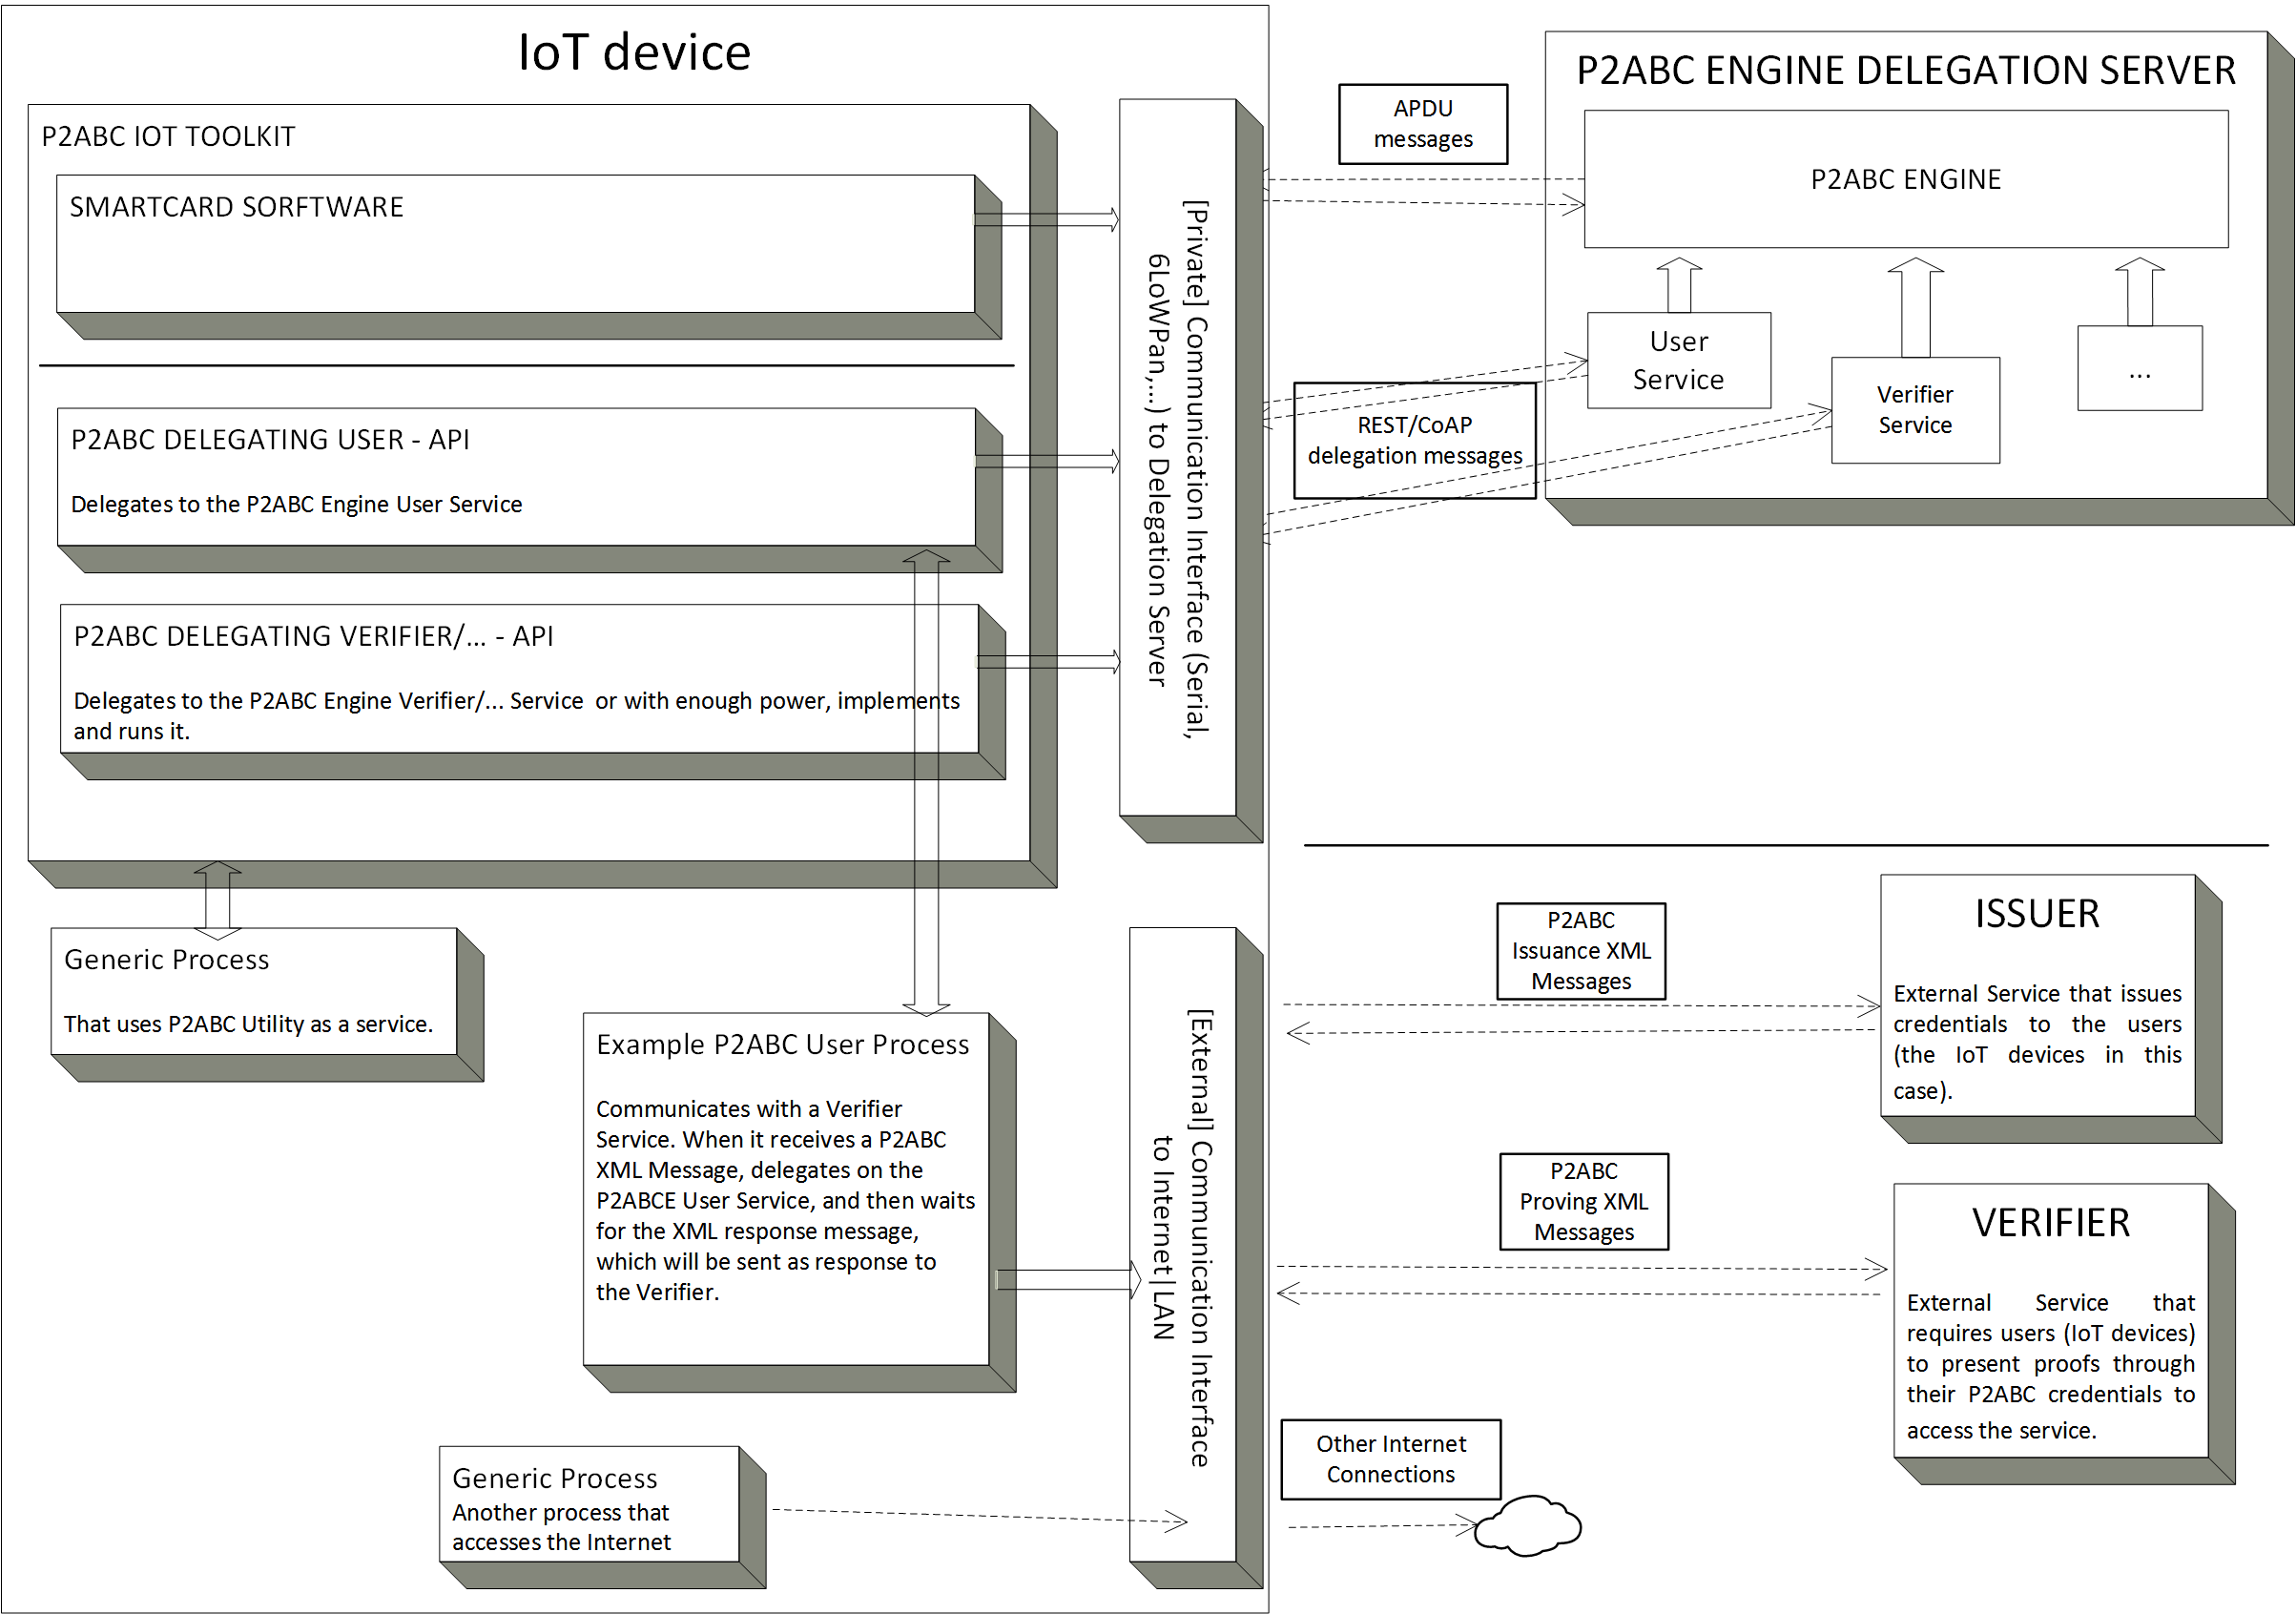
\includegraphics[width=\linewidth]{gfx/P2ABCE-IoT-bw}
	\end{center}
	\caption{IoT in P2ABCE Architecture.}
	\label{fig:P2ABCE-IoT}
\end{figure}

%\begin{figure}[bth]
%	\begin{center}
%		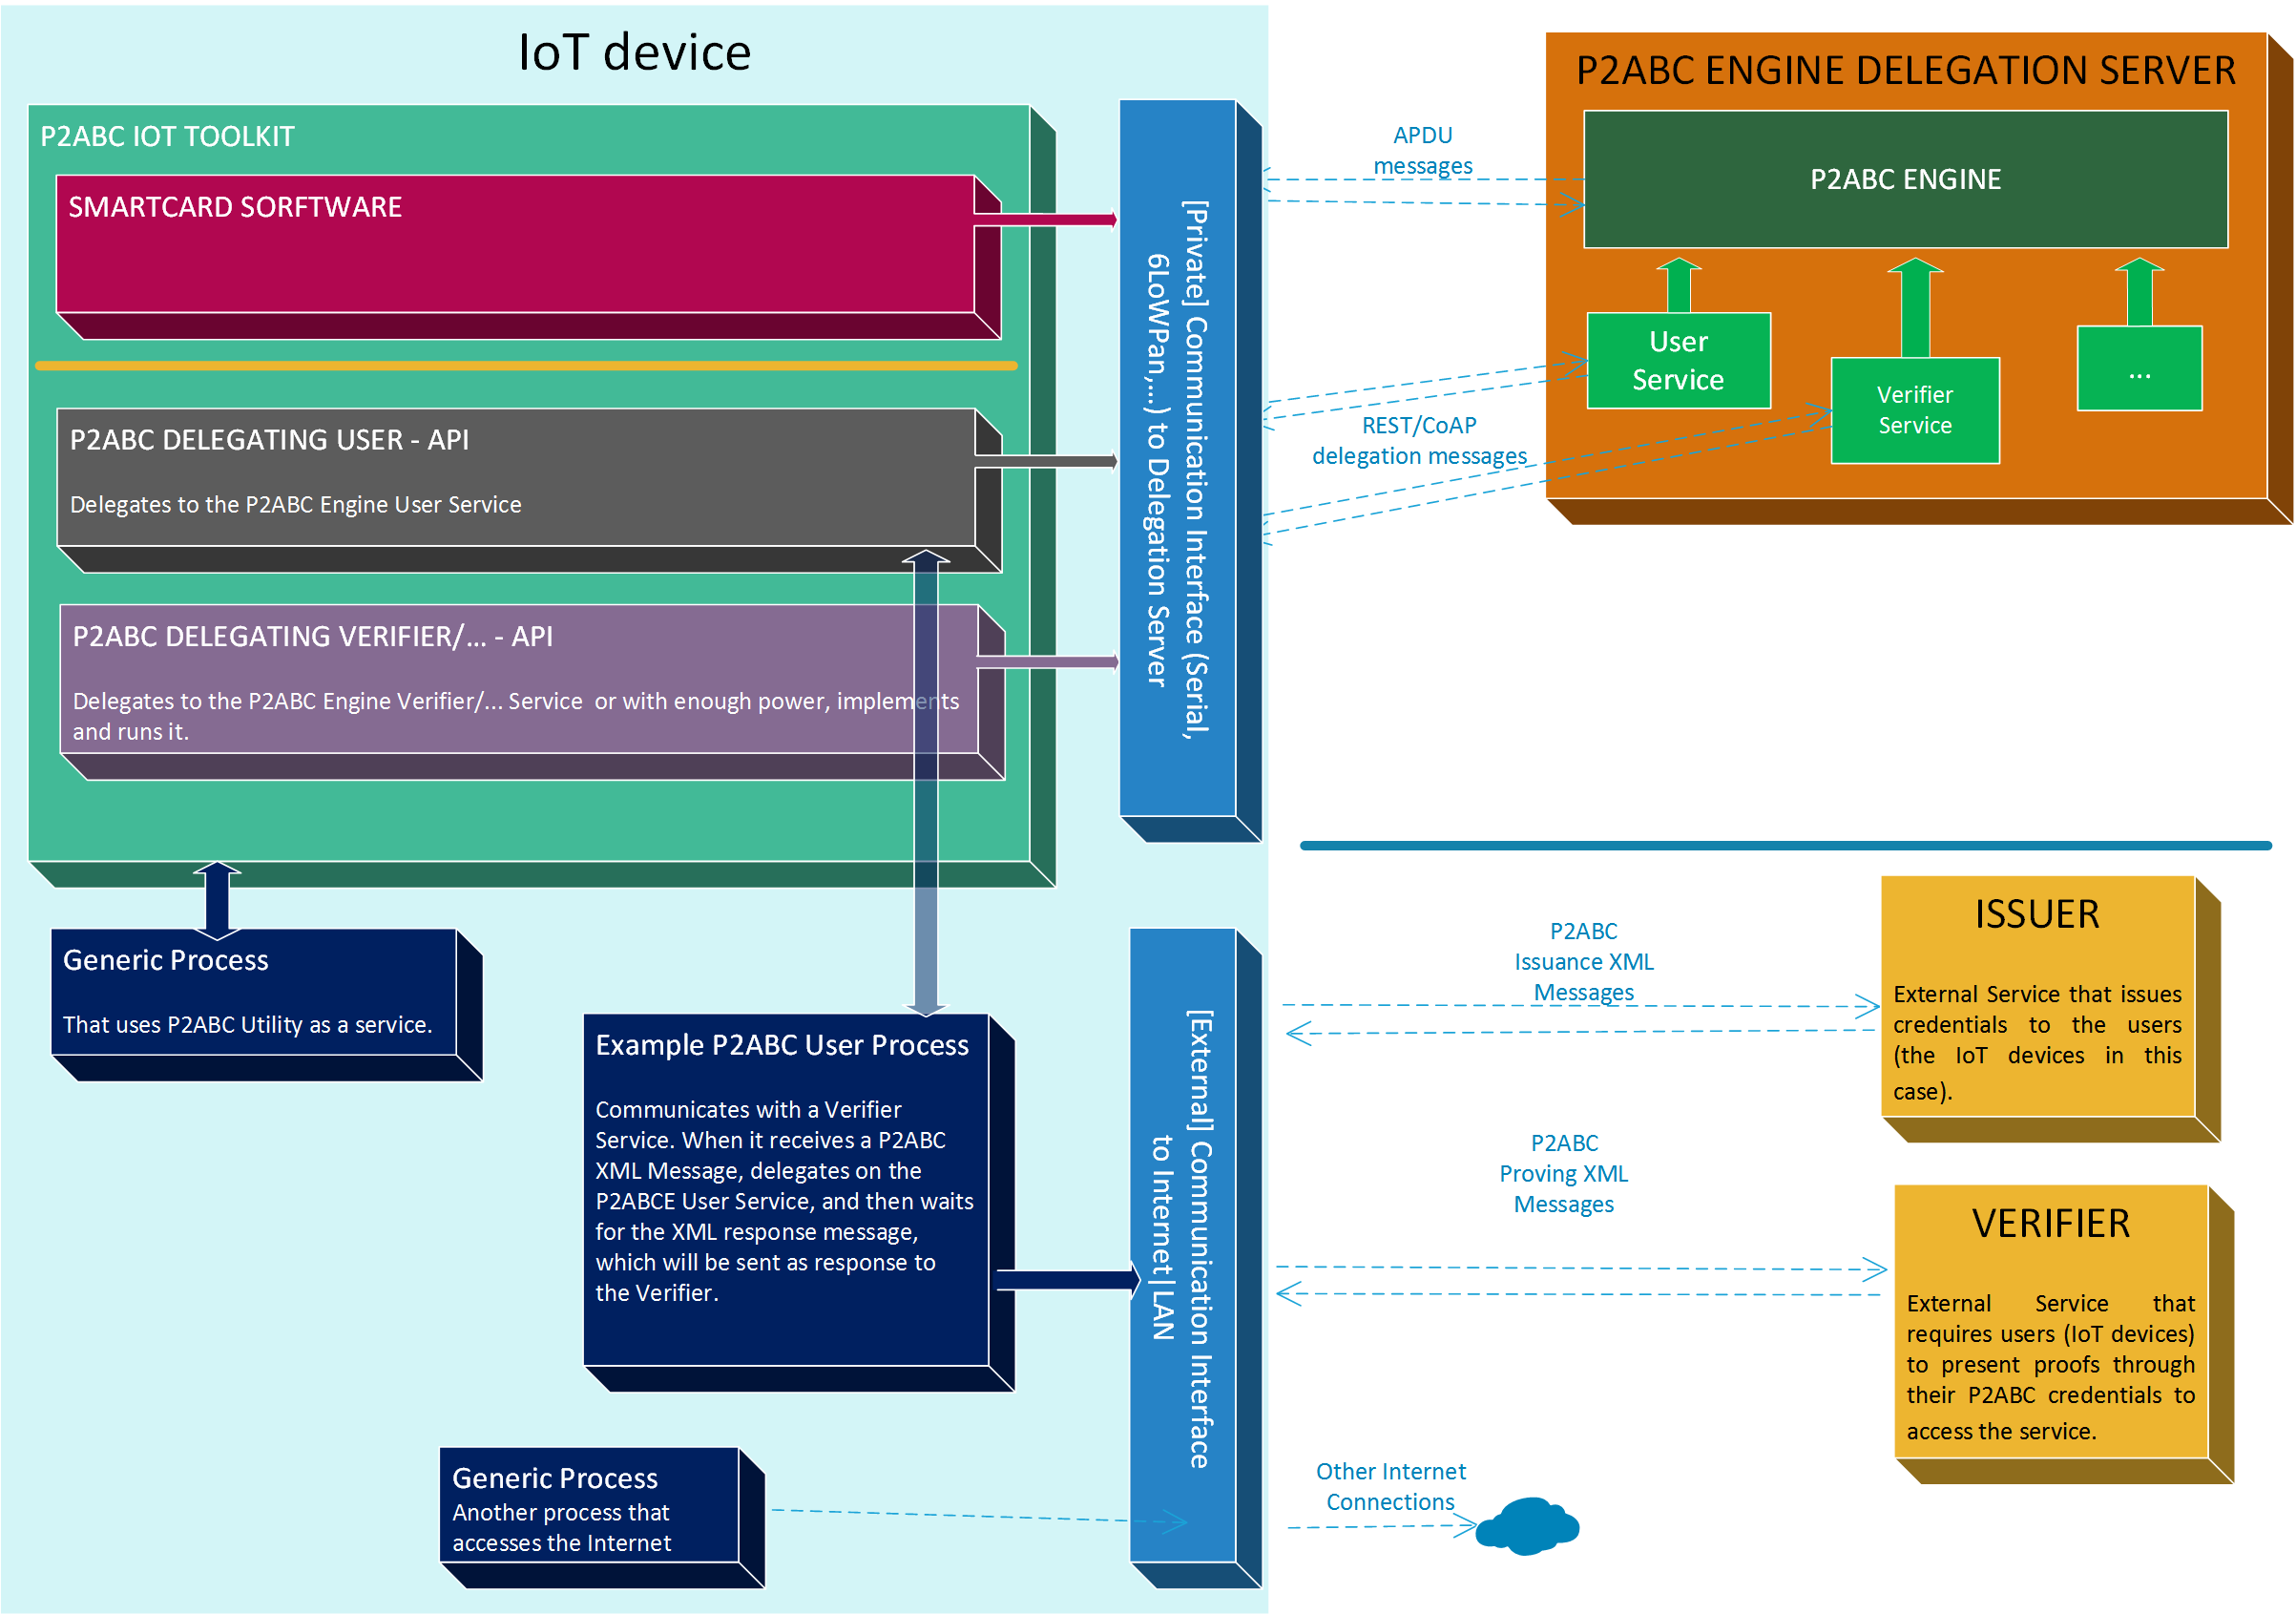
\includegraphics[width=\linewidth]{gfx/P2ABCE-IoT-color}
%	\end{center}
%	\caption{IoT in P2ABCE deployment diagram.}
%	\label{fig:P2ABCE-IoT-color}
%\end{figure}

\hfil


The system will be compounded by the IoT device, the P2ABCE delegation server and the third party P2ABCE actors.

\begin{itemize}
	
	\item \textbf{IoT device}
	
	In \autoref{fig:P2ABCE-IoT} the IoT device is represented with two interfaces, physical or virtual. One allows external communications to other machines, including other P2ABCE actors, that could be on the Internet, a corporate LAN, a M2M overlay network, etc. Through this interface, the P2ABCE XML messages are exchanged as in any other deployment. This allows an IoT device to interact with other actors without special adaptations to the protocol. The other interface allows a secure communication with the delegation server. Both the delegation messages and the APDU Dialogue are transmitted over this interface, making it a point of attack to the system, and we will talk about its security in the delegation process.
	
	The scheme also shows the \textit{P2ABCE IoT Toolkit}. This piece of software includes the IoT Smart Card, and the API for other processes that want to use the P2ABCE system.
	
	The IoT Smart Card is the implementation of a software smart card, listens for APDU Commands from the secure interface and stores securely the credentials and private keys within the device's memory.
	
	The P2ABCE API is an interface for other processes that wish to use the private-preserving environment of P2ABCE. It provides access to every operation available, hiding the delegation process. In the future, if for example the Verification Service is implemented for the IoT device, i.e., there's no need to delegate to other machine to act as a Verifier, then any program using the API won't need to change anything, the toolkit conceals the transition from delegating to native execution.
	
	
	\item \textbf{P2ABCE actors}
	
	If we recall from \autoref{analysisP2ABCE}, the possible roles in the system were the Issuer, the User, the Verifier, the Revocation Authority and the Inspector. All of them use the P2ABCE XML schema in the specification to communicate to each other. Any third party actor will be unaware of the fact that the device is a constrained IoT device that delegates on the P2ABCE server.



	\item \textbf{P2ABCE Delegation Server}
	
	The machine in charge of receiving authorized IoT devices' commands to parse the XML files exchanged and orchestrate the cryptographic operations the IoT smart card must perform.


\end{itemize}

\hfil

\begin{flushleft}
	\textbf{Delegation process}
\end{flushleft}

Here we describe the computation offloading carried out by the IoT device.  In \autoref{fig:DelegationProving} we show an example of the IoT acting as a User, Proving a Presentation Policy to a third party Verifier.

\begin{enumerate}
	\item Communication with P2ABCE actor.
	
	The IoT device starts an interaction with another actor, e.g. an Issuer or Verifier, receiving a P2ABCE XML file.
	
	
	\item Delegation to the P2ABCE Server.
	
	Depending on what role the IoT device is acting as, it will delegate in the corresponding service, e.g. User Service. The delegation message must include the XML file, and any parameter required to accomplish the task, like the information on how to communicate with the IoT smart card (listening port, security challenge, etc.).
	
	\item APDU Dialogue (if necessary).
	
	The server may need to send APDU Commands to the IoT smart card to read the credential information or perform cryptographic operations involving private keys.
	
	\item Server response.
	
	The server may return a status code or a XML file if the first one required an answer from the IoT device, in which case, it will send as response to the third party actor, resuming the communication.
	
\end{enumerate}

\begin{figure}[bth]
	\begin{center}
		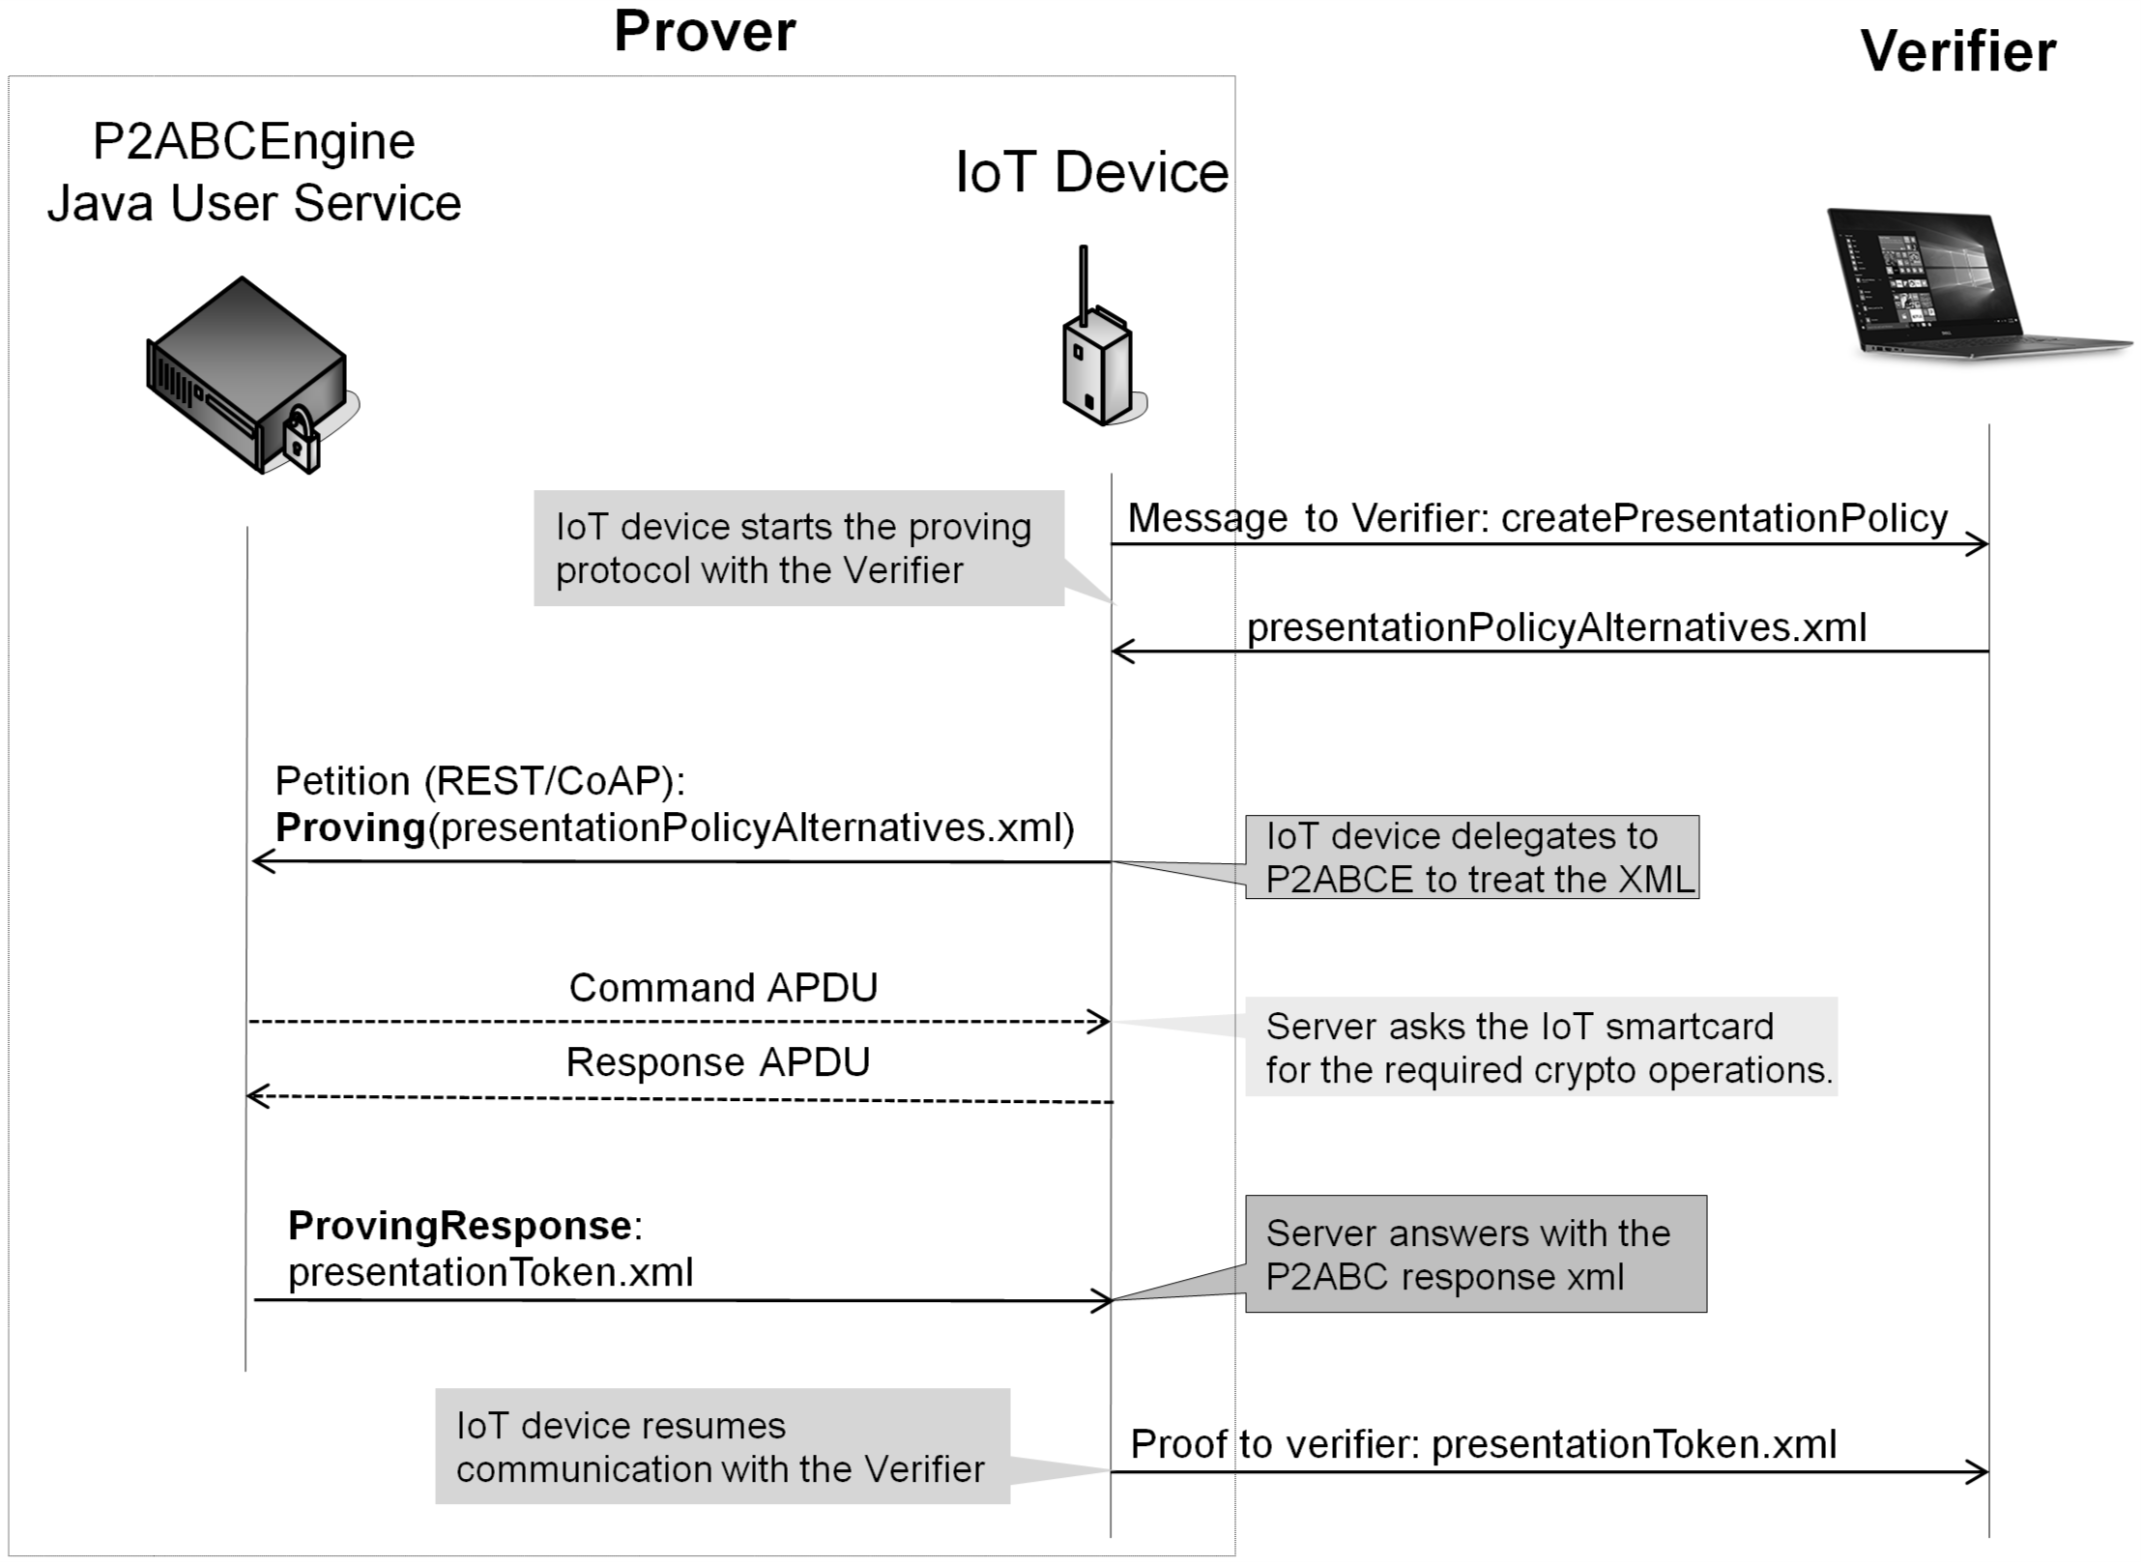
\includegraphics[width=\linewidth]{gfx/UML/DelegationProving}
	\end{center}
	\caption{IoT Delegation in P2ABCE for Proving.}
	\label{fig:DelegationProving}
\end{figure}

Transmissions over the \textit{Server-IoT} channel must be secured in order to avoid attacks like: impersonate the P2ABCE delegation server, having access to the IoT smart card sending the APDU Commands the attacker wishes; delegate as a device on the server but giving the parameters of another device, making the delegation server send the APDU Commands to a victim IoT smart card.


We could use a corporative PKI to issue certificates to the server and devices and configure policies for access control; design a challenge-response system combined with the smart card PIN, like a password and TOTP\footnote{Time-based One-time Password} in a 2FA\footnote{Two-factor authentication} login. We also could connect physically the delegation service through RS-232 serial to the IoT device, securing both physically as we would do with the IoT device on its own, isolating the delegation system from any network attack. This last idea is an approximation to the Arduino Yún\footnote{\url{https://www.arduino.cc/en/Main/ArduinoBoardYun}}, a development board that integrates two microcontrollers, one a typical Arduino with very low resources, and another one running a fork of OpenWrt. The Arduino microcontroller can control the terminal of the more powerful one, using the serial pins as commented before.

As we can see, there are many state of the art solutions for all this threads, therefore, we can assume a secure channel without mentioning a specific solution, providing freedom to choose the most fitting one in a real deployment.


\paragraph{Notes for more constrained devices}

Our architecture is designed for devices that could in a future run a reimplemented version of P2ABCE, that means, the devices could perform more tasks than only running the smart card software and their main purpose process, e.g. recollecting sensor data. But if our target devices are so constrained that can barely run the smart card, they may not be able to handle the XML files because of memory restrictions, like a MSP430\footnote{\url{http://www.ti.com/lsds/ti/microcontrollers-16-bit-32-bit/msp/overview.page}} running Contiki-OS, the microcontroller has between hundred of bytes to tens of kilobytes of memory, making impossible to store multiple XML files in the size range of tens of kilobytes.

In these cases, the delegation in the server goes a step forward, making the server a proxy to communicate with other P2ABCE actors, and the IoT device only acts as a smart card. The IoT device would still act as the User, or any other P2ABCE, role because it orchestrates when and how an interaction with other actor is executed, but the communications would be between the proxy and the third party actor. 



\section{Proof of Concept Implementation}
% +Implementation:
% *System:
% 	-Raspbian OS: distro de debian para Raspberry Pi, que se describirá en los tests
% 	-LEDE: ash terminal (shell command interpreter), POSIX, typical hardware, libraries with no hardware aceleration vs smart card MULTOS,
%
% *Delegation
%  -REST as current delegation protocol: curl script bash
%  -BIOSC as current APDU transmission protocol: no security -> no overload.
% *Smart Card
%  
%  -IoT Smart Card software design and implementation notes.
%  -Sequence diagrams. TODO


In this section we present the first PoC implementation, introducing the IoT system where we are going to work, then we will describe the delegation protocols, one for the computation offloading of the IoT device on the P2ABCE server, and another for the transmission of APDU Commands, and finally, we will describe the IoT smart card implementation.



\subsection{IoT system}

We will develop our PoC in Linux based systems in order to avoid complications with firmware specific issues that we are not familiar with. Even so, the linux systems used are aimed for the IoT environment and serve as a starting point for future implementations in more constrained devices or different systems.

In our delegation server we will run Raspbian OS, a distribution based on Debian for the Raspberry Pi. We will talk more about the hardware specifications in the benchmark chapter. We chose this system because it has a great package repository support, including the Java Runtime Environment, needed to run the P2ABCE Services.

For our IoT device, we will use LEDE, Linux Embedded Development Environment, a distribution born from OpenWrt, aimed for routers and embedded chips with low resources requirements. It offers the \texttt{ash} command interpreter, or \texttt{shell}, and the \texttt{opkg} package manager, that allows an easy installation of some libraries and tools needed during the early development.











\subsection{PoC Delegation}

As we explained in the design section, the delegation has two steps, the IoT device calling the P2ABCE server to offload the parsing of the XML data, and the P2ABCE server sending APDU Commands to the IoT smart card in the device.




\subsubsection{PoC Delegation to the P2ABCE Server}


Currently P2ABCE offers multiple REST web services to run different roles in P2ABCE system: User Service, Issuer Service, Verification Service, etc. Any third party application that integrates P2ABCE with their system can make use of these services or implement the functionality using the library written in Java, the tool that the REST services actually use.


Our PoC machine, the Omega2, can make REST calls easily with the \texttt{curl} command, but other devices may use \ac{CoAP}, but in that case, the P2ABCE REST services should be adapted to offer CoAP support. The commands needed to delegate to the P2ABCE server would be the same that those defined now to operate with the REST services, but with the modifications needed to pass the parameters on how to communicate with the IoT smart card.

In this PoC the only P2ABCE Service that needed to be modified was the User Service. We added the following REST call

\begin{center}
	\textit{/initIoTsmartcard/{issuerParametersUid}?host=\&port=}
\end{center}

where we communicate the P2ABCE server that an IoT Smart Card is accessible via \textit{host} and \textit{port}. Then a new \textit{HardwareSmartcard} object is stored in the P2ABC Engine, but instead of the \textit{javax.smartcardio} Oracle's \textit{CardTerminal} implementation, we use our own \textit{IoTsmartcardio} implementation for the \textit{HardwareSmartcard} constructor, that we will discuss in the following section.


\hfil

In a real deployment, we would offer a full library with an API for other processes that want to use the P2ABC Engine, which automatizes the boot of the IoT smart card and handles the security policies, like the one we presented in the deployment diagram \ref{fig:P2ABCE-IoT} of the \textit{P2ABCE IoT Toolkit}.

Now we show some examples of the PoC \texttt{curl} commands, run in the device's terminal, or from a shell script for automation:

\begin{lstlisting}[language=bash]
$ curl -X POST --header 'Content-Type: text/xml' "http://$DelegationServerIP:9200/user/initIoTsmartcard/http%3A%2F%2Fticketcompany%2FMyFavoriteSoccerTeam%2Fissuance%3Aidemix?host=192.168.3.1&port=8888"

$ curl -X POST --header 'Content-Type: text/xml' -d @firstIssuanceMessage.xml "http://$DelegationServerIP:9200/user/issuanceProtocolStep/" > issuanceReturn.xml
\end{lstlisting}

The IoT device will only manage XML as data files to exchange between the third party actor and the P2ABCE delegation service, attaching them in the body of the REST call. In the parameters of the first call we can see the IP and port where the IoT smart card will be listening.



\subsubsection{APDU Dialogue Transmission}


To transmit the APDU messages in our PoC we use a simple protocol, that we will refer as BIOSC (Basic Input Output Smart Card), consisting in one first byte for the instruction: 

\hfil

\begin{tabular}{|c|l|}
	\hline
	\texttt{0x01} & APDU Command or Response: Read 2 bytes for the\\& length and then as many bytes as said length. \\
	\hline
	\texttt{0xff} & Finish connection: close the current TCP socket and\\& end the IoT smart card execution. \\
	\hline
\end{tabular}

\hfil

In the first instruction, we read two header bytes with the length of the APDU Command or Response to receive, followed by said APDU bytes. The message is sent over TCP for a reliable transmission (concept of session, packet retransmission, reordering, etc.). The second instruction serves for closing the TCP socket in the IoT device when the smart card is no longer needed.

We lack any security (authentication or authorization) that a real system should implement. It is vital to authenticate the delegation service, to authorize it to make APDU Commands, and the same with the IoT device, to prevent attacks. But using this method for the transmission of the APDU messages, with only 3 bytes of overhead, helps us in the  benchmarks to measure the real performance of the system.


\hfil


The implementation of this simple protocol is done in both Java and C, one for the P2ABCE server and the other one for the IoT smart card.

\hfil

As we mentioned in the analysis of P2ABCE's code, the \texttt{HardwareSmartcard} class implements the \texttt{Smartcard} interface using the package of abstract classes \texttt{javax.smartcardio} to communicate with the physical smart cards. The Oracle JRE implements these package for the majority of smart card manufacturers. For our PoC, we implement the \texttt{javax.smartcardio} package so it transmits the APDUs with BIOSC, making the use of a physical or IoT smart card totally transparent to the \texttt{HardwareSmartcard} class, enhancing maintainability, and following the \textit{expert pattern} from the known GRASP guidelines.

%TODO : optional: diagrama secuencia de P2ABCE, pero si eso solo de la reimplementación de javax.smartcardio y su uso por HardwareSmartcard

\textbf{TODO} :  diagrama secuencia de la reimplementación de javax.smartcardio y su uso por HardwareSmartcard

\hfil


In the PoC IoT device, we implement in \texttt{BIOS.c} the \texttt{main()} function, that reads from a Json file the previous status of the smart card, and then opens the TCP socket in the $8888$ port, and loops listening for BIOSC transmissions until an $0xff$ is received. When an APDU Command is sent, it calls the APDU Handler, that we will talk about in the next section.




\subsection{IoT Smart Card Implementation}


After many design decisions in the process to adapt the original ABC4Trust Card Lite code to pure C, working on a MIPS architecture, in this section, we present the current \ac{PoC} code, most important decisions taken and the execution workflow in the form of sequence diagrams.


\hfil



\subsubsection{Code structure}


We divide the project in three different sections with the objective of enhancing maintainability, improving future changes, ports, fixes, etc.

In \autoref{fig:IoTCScomponents-bw} we show the project's structure. The first section is what could be called as the core of the smart card, the second one the interface for those tools the core needs and that may depend on the target's platform, and finally, the third party libraries, that may be empty if the interfaces implementation doesn't require any.




%\begin{figure}[bth]
%	\begin{center}
%		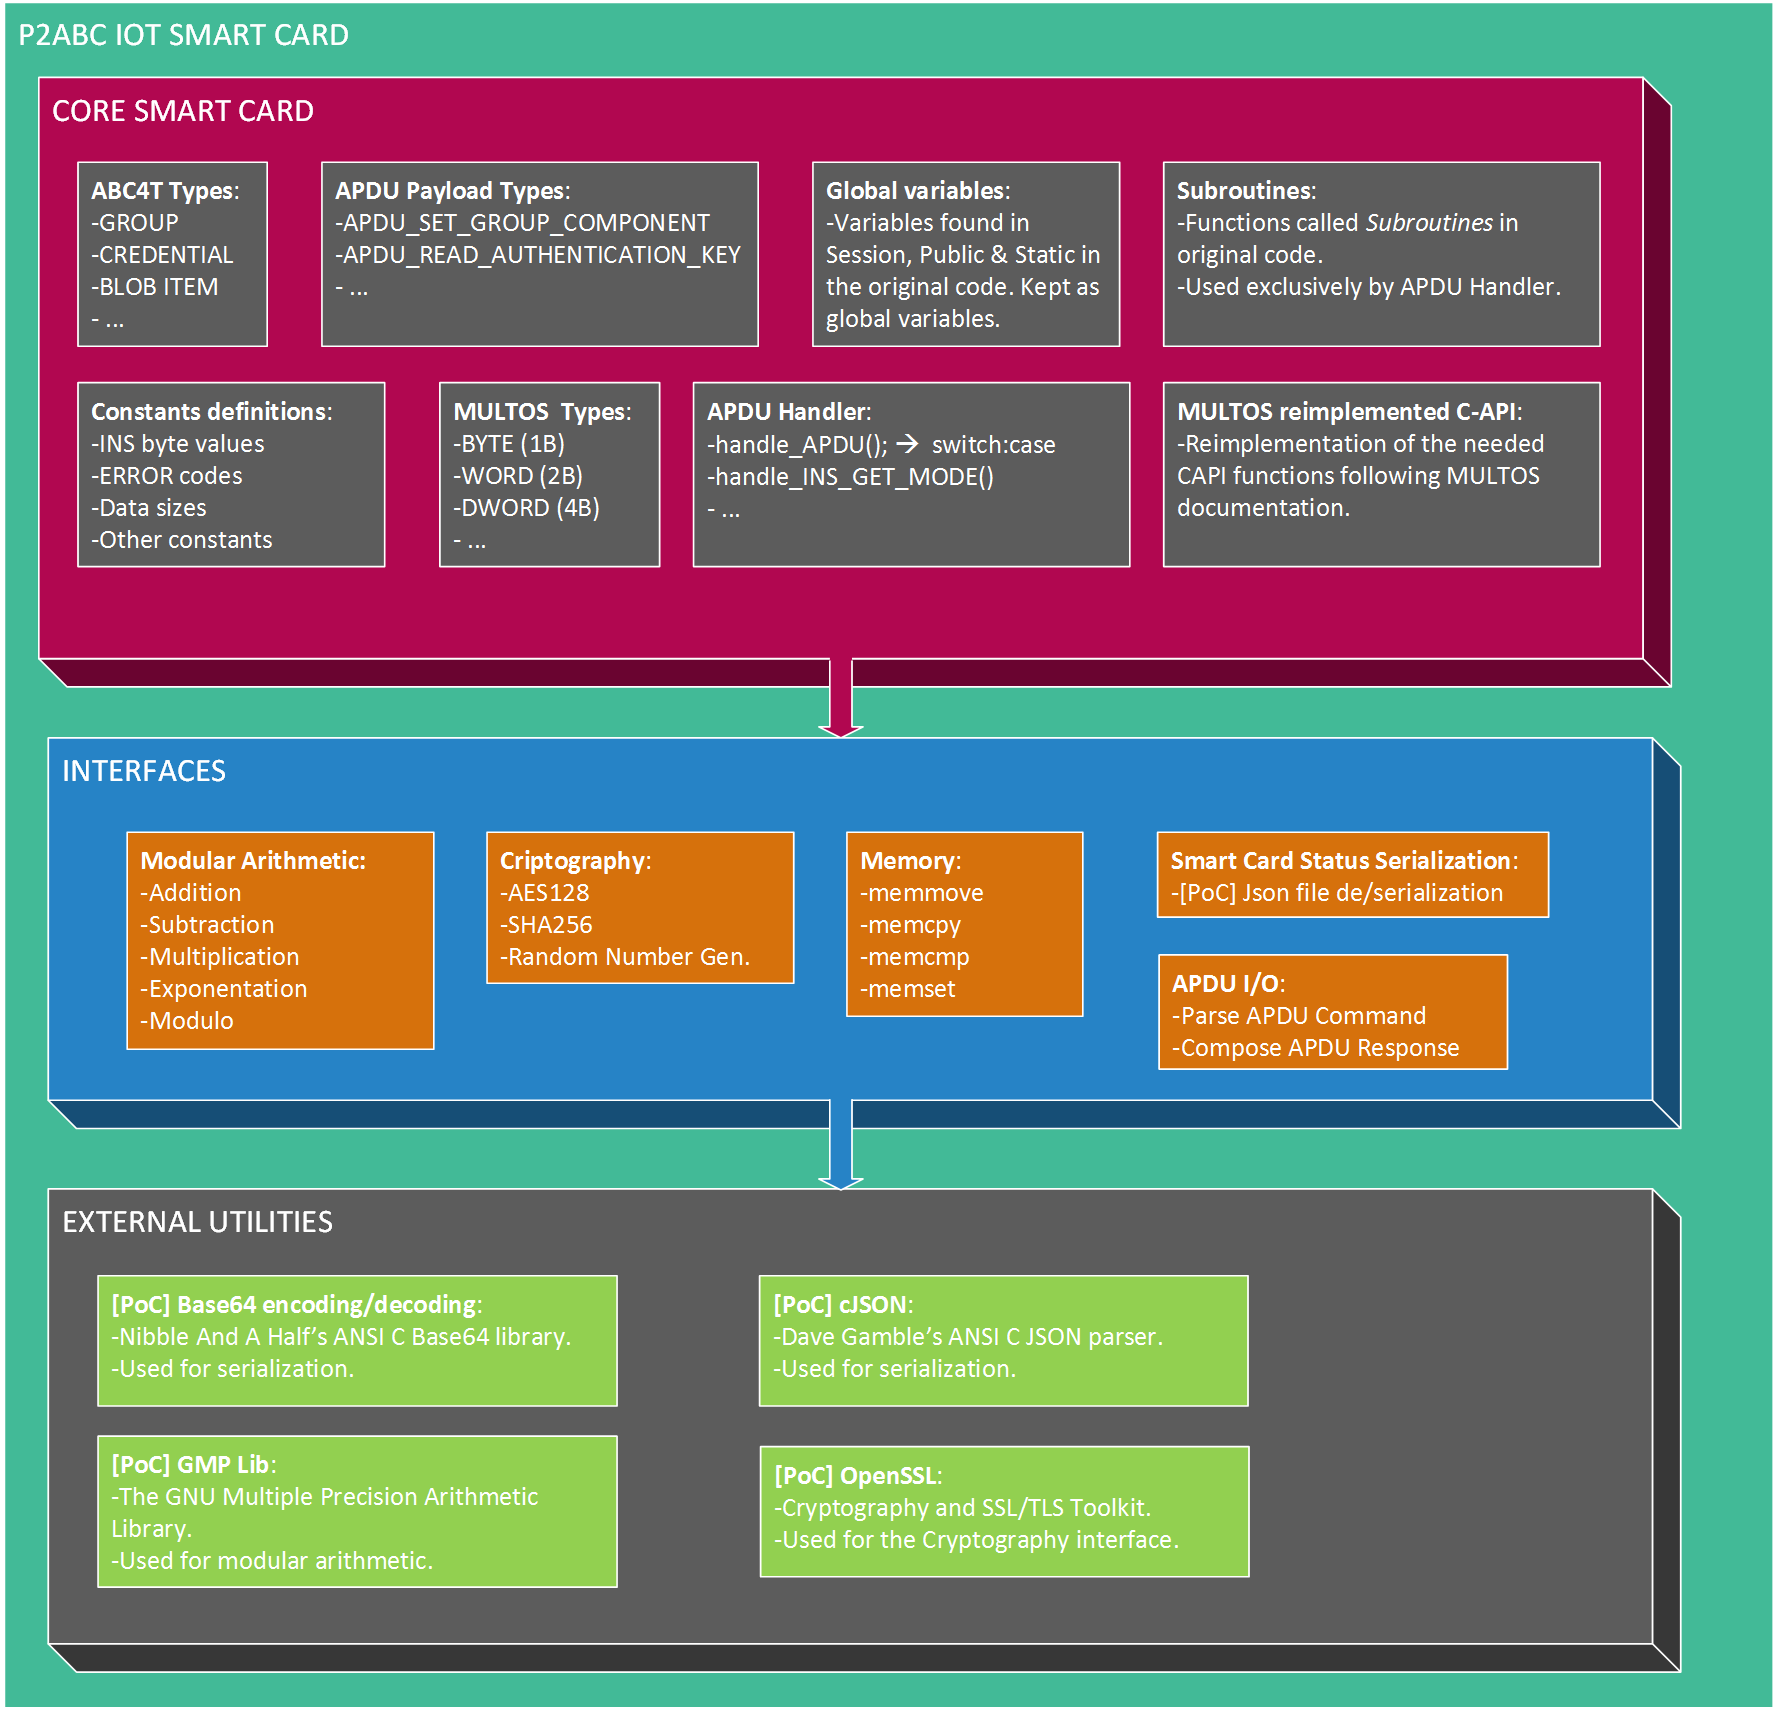
\includegraphics[width=\linewidth]{gfx/IoTCScomponents-color}
%	\end{center}
%	\caption{IoT Smart Card Code Structure.}
%	\label{fig:IoTCScomponents-color}
%\end{figure}

\begin{figure}[bth]
	\begin{center}
		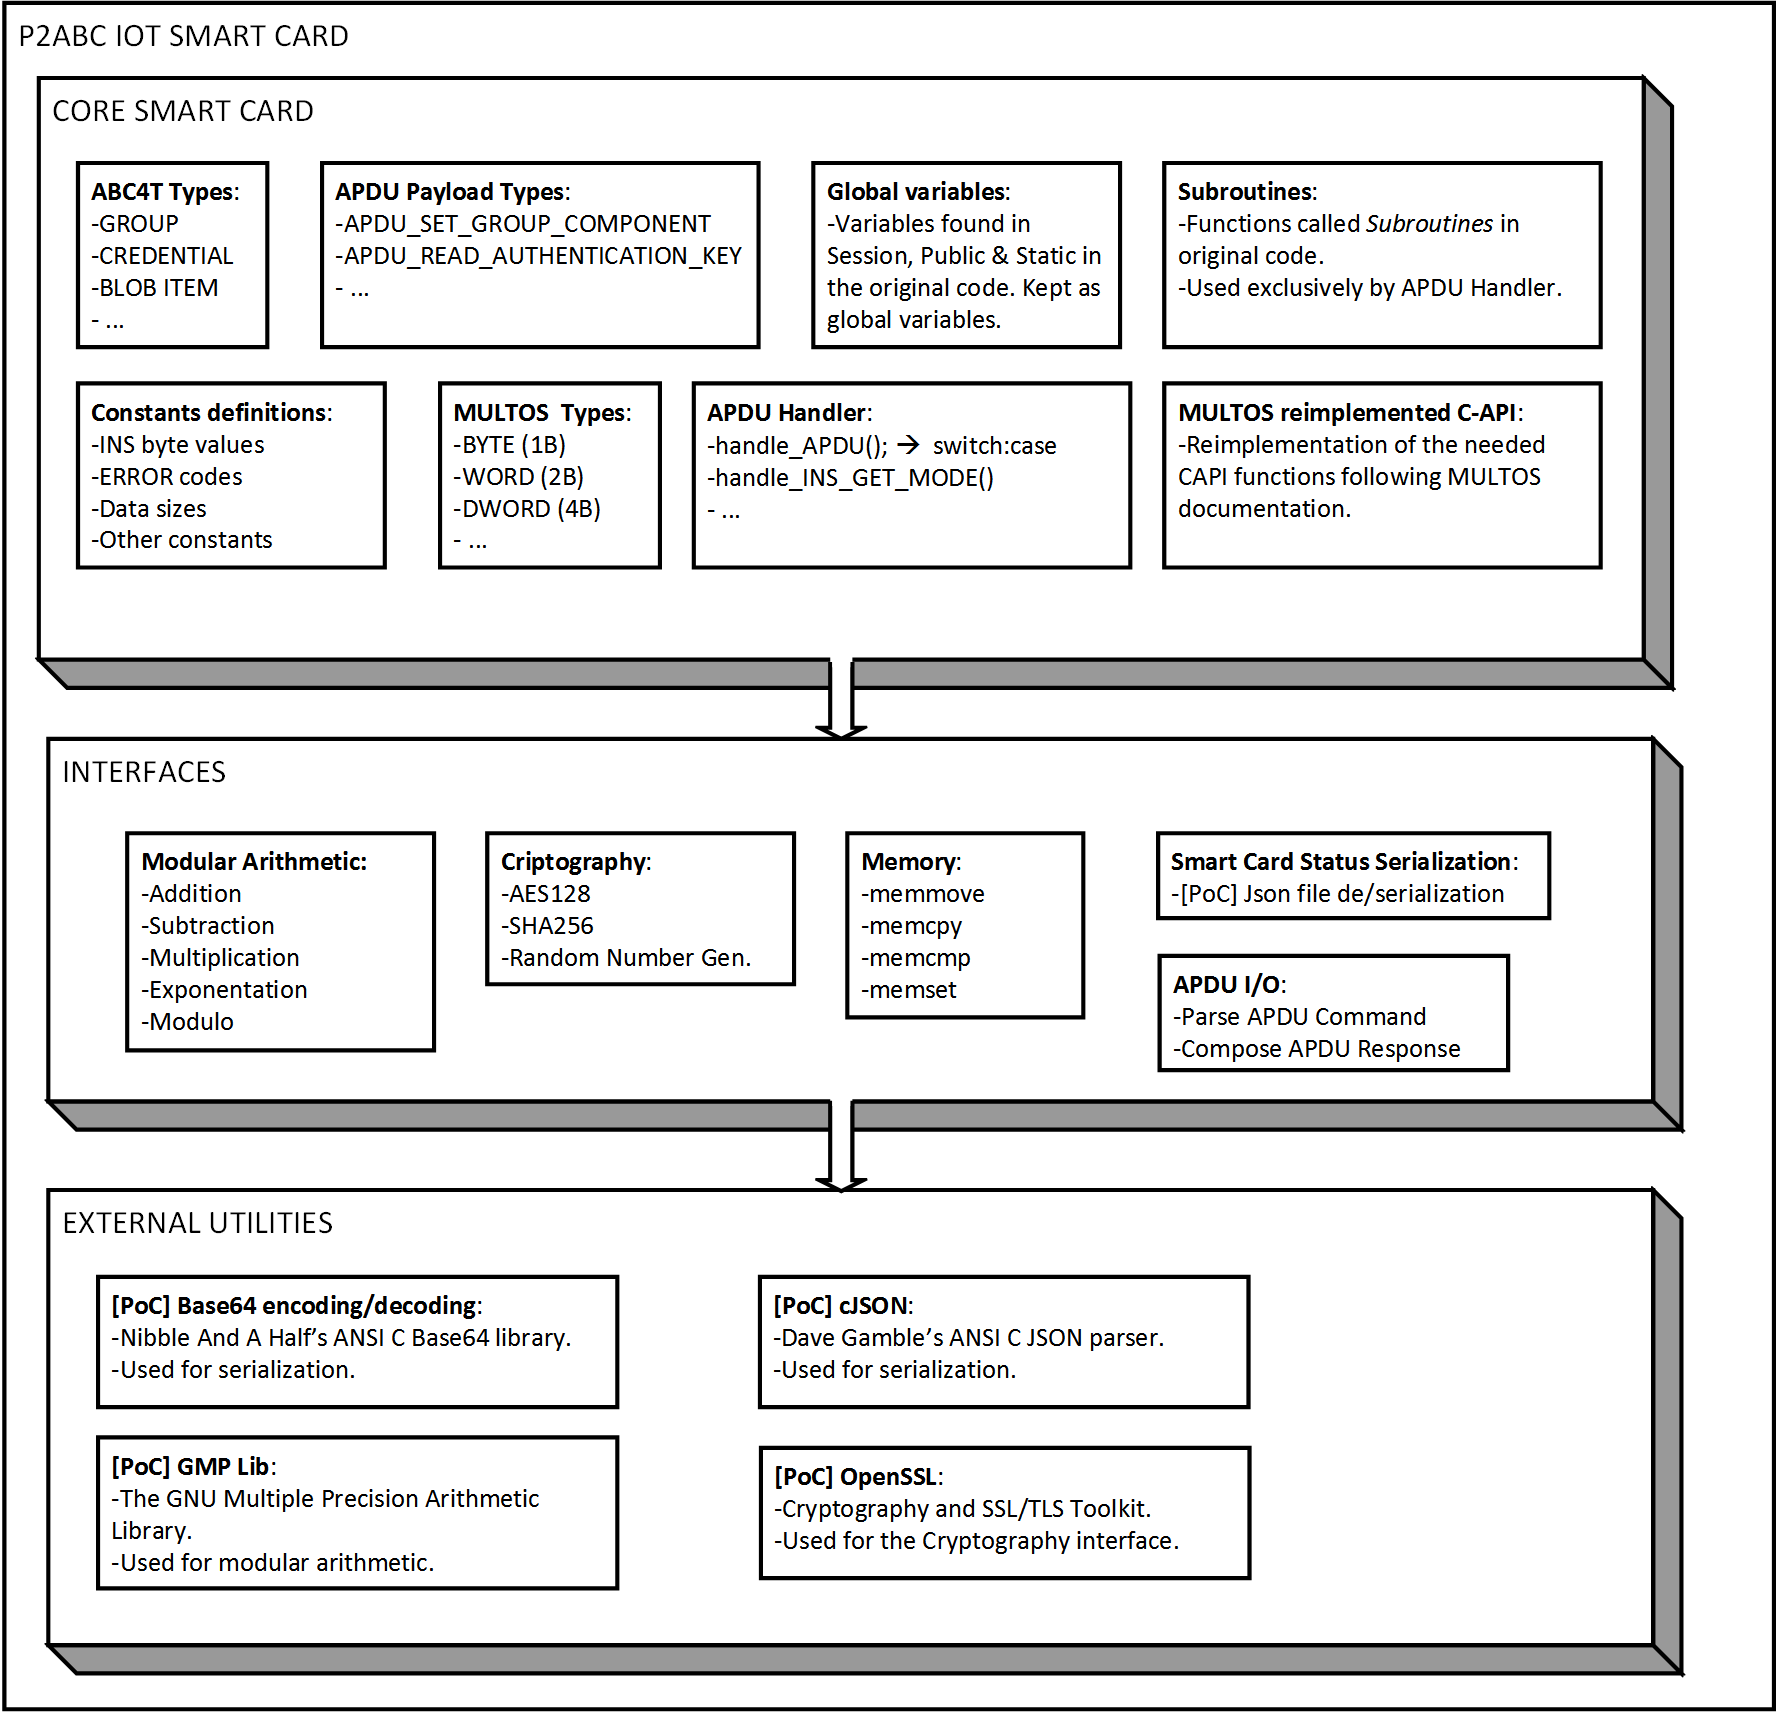
\includegraphics[width=\linewidth]{gfx/IoTCScomponents-bw}
	\end{center}
	\caption{IoT Smart Card Code Structure.}
	\label{fig:IoTCScomponents-bw}
\end{figure}


\hfil

\paragraph{Core smart card}
\hfil

The smart card logic lies in this section, the concepts of APDU Commands, what instructions are defined for P2ABCE smart cards, and how to process them and generate proper APDU Responses.

If the APDU protocol defined for P2ABCE smart cards changed, with the consequence of having to update all smart cards in use, the changes to adapt the IoT smart card should be applied in this part of the code. This also implies that if the P2ABCE Java code changes their \texttt{Smartcard} interface, something more probable, the IoT smart card will still work as intended.

Most of the original ABC4Trust Card's code has been reused in this section, e.g., all the global variables and custom data type definitions, the APDU Command handling and auxiliary subroutines.

However, the ABC4Trust's code heavily depended on the MULTOS platform for the input and output of data, modular arithmetic, memory management, and AES128 and SHA256 cryptographic operations. Therefore, we reimplement the used MULTOS functions following the documentation, adapting it in some cases.

A characteristic of MULTOS C-API is that every function name starts with ``\texttt{multos}'', so we changing their names from \texttt{multosFoo()} to \texttt{mFoo()} for readability and to emphasize that they were no longer MULTOS functions.

The \texttt{main.h} file, from the original ABC4Trust project, also implemented some functions that were equivalent to the ones available in \texttt{multos.h}. We replaced them for the standard functions in the C-API, checking that the MEL code did the same as the documentation specified. This last detail is very important, because in \citep{vullers2013efficient} they noted that MULTOS' \texttt{ModularExponentiation} function does not accept exponents larger than the modulus size, so they implemented \texttt{SpecialModularExponentiation}, dividing the exponentiation in two that MULTOS could perform. After this analysis, when those particularities appeared, our reimplementation of the MULTOS API accepts the \textit{expanded functionality}.

\hfil

Because of the inherited code, many particularities of the internals of the MULTOS platform had to be addressed. 

One was the different memory zones, where the variables in \texttt{static} were read and written directly from the secure EEPROM, defining the status of the smart card between executions. We keep those variables in RAM, but save them in a Json file, deserializing them at the smart card boot up, and serializing always before an APDU Response is sent. From the MULTOS documentation, the \texttt{static} variables are read and written atomically, and if power source is lost during any process, memory won't get corrupted. This also means that if a MULTOS smart card sends an APDU Response, every variable that had to change, is saved in the EEPROM. Our PoC uses Json for human readability during debugging, but a real deployment should apply secure reads and writes on the file, preventing data corruption and undesired access, for example, ciphering the file with a key derived from the smart card PIN. It is also desirable another data serialization method, reducing the size of the file to store in memory constrained devices.


Another of the mentioned particularities is that the MULTOS compiler does not apply padding between variables in the data structures. For example, in an X86 machine, where a \texttt{short} is stored in 2 bytes, in the following code\footnote{From \url{https://en.wikipedia.org/wiki/Data_structure_alignment}}

\begin{lstlisting}[language=C]
	struct MyData
	{
		short Data1;
		short Data2;
		short Data3;
	};
\end{lstlisting}

each member of the data structure would be 2-byte aligned. Data1 would be at offset 0, Data2 at offset 2, and Data3 at offset 4. The size of this structure would be 6 bytes. But if we defined the following structure

\begin{lstlisting}[language=C]
	struct MixedData
	{
		char Data1;
		short Data2;
		int Data3;
		char Data4;
	};
\end{lstlisting}

where a \texttt{char} is 1 byte, and an \texttt{int} uses 4 bytes, although the total bytes used are 8 bytes, the compiler will align them in memory adding padding, like if we defined the following:

\begin{lstlisting}[language=C]
struct MixedData  /* After compilation in 32-bit x86 machine */
{
	char Data1; /* 1 byte */
	char Padding1[1]; /* 1 byte for the following 'short' to be aligned on a 2 byte boundary
	assuming that the address where structure begins is an even number */
	short Data2; /* 2 bytes */
	int Data3;  /* 4 bytes - largest structure member */
	char Data4; /* 1 byte */
	char Padding2[3]; /* 3 bytes to make total size of the structure 12 bytes */
};
\end{lstlisting}



\hfil


In MULTOS, to reduce the memory usage, there is no padding, and this affects the inherited ABC4Trust's code because of the use of \texttt{memcpy} to copy zones of memory from one address to another. The problem is the code copies multiple variables in one \texttt{memcpy} call, because, for example, the APDU Command payload includes multiple data, and instead of copying one variable at a time, the \texttt{struct} is defined with the same order and copies everything at once.

An example taken from the parsing of instruction \texttt{SET\_PROVER}:

\begin{lstlisting}[language=C,frame=tblr]
typedef struct
{
	BYTE prover_id;
	unsigned int ksize;
	unsigned int csize;
	BYTE kx[MAX_SMALLINT_SIZE];
	BYTE c[HASH_SIZE];
	BYTE proofsession[PROOFSESSION_SIZE];
	BYTE proofstatus;
	BYTE cred_ids[NUM_CREDS];
	BYTE cred_ids_size; // also called 't' in the documentation
	BYTE exists;
} PROVER;
/*****/
PROVER provers[NUM_PROVERS];

/*****/
case INS_SET_PROVER:
  // [...]
  memcpy(&(provers[temp_prover_id-1].prover_id), &(apdu_data.set_prover_in.prover_id), 5); // under the hood, this also initializes ksize and csize
\end{lstlisting}
This is the only case where a comment showcases that it is copying more than one byte.

The temporal solution is to use \texttt{struct \_\_attribute\_\_((\_\_packed\_\_))} to ask a GCC compiler to not use padding in the structs, but this is not standard, neither a good practice. A deeper refactorization of the code is needed where the hidden copies of variables are made explicit, letting the compiler manage the memory layout.


\hfil

An internal alarm should always warn us when we see raw memory copy from serialized data, that is, the APDU Payload. We mentioned in the MULTOS introduction that the platform is Big Endian. The serialized data is also typically represented in Big Endian, and our APDU Payloads do so. In our code we added a new Subroutine to check whether the device is Big or Little Endian, and to rectify the Endianness from those variables, with 2 or more bytes (the only ones affected by the Endianness), copied from or written to APDU Payloads.


\hfil


Finally, we must talk about the \texttt{multosExit} function. In a MULTOS application, to finish the execution and send the APDU Response, the programmer can call in any moment to \texttt{multosExit}, and the MULTOS OS will continue the execution, not returning to the application again.

Think about how we all have, at least once, used an \texttt{if} and \texttt{return} to avoid the \texttt{else}, like in this example:

\begin{lstlisting}[language=C]
if(condition)
	return a;
return b;
\end{lstlisting}


The use of \texttt{multosExit} in ABC4Trust code is similar, but used in almost every function. This leads to a sequence execution with many possible interruptions, leaving a full stack behind with \textit{un-returned} function calls, i.e., parameters stored in memory after a function call that never returns. In MULTOS, this memory won't affect future executions, because with the next APDU Command, the stack will be loaded with the clean application, and the Session memory stays untouched between APDU Commands, during an APDU Dialogue. 

To adapt the code, the reimplemented \texttt{mExit} function can not end the program execution, because we would lose the variables in RAM needed during the APDU Dialogue, as well as that the TCP socket would close. The solution is to refactor every use of \texttt{multosExit} in a way that, if it is called from a Subroutine, the function returns a success or error code, and the only functions that can call \texttt{mExit} are the ones handling an specific instruction.

Nevertheless, there is one exception, the \texttt{output\_large\_data()} Subroutine, which is a tool to send large data payloads without Extended APDU support. We talked about this in \ref{subsec:APDU}, mentioning the special instruction \texttt{GET RESPONSE}.

Summarizing, every Subroutine must return from its execution, as well as every instruction handler, which must call either \texttt{mExit} or \texttt{output\_large\_data()} before returning. After the instruction has been handled, the execution returns to the listening loop of BIOSC.



\paragraph{Interfaces}\hfil

To reimplement some of the MULTOS functions, we needed to use some libraries, so we defined a facade to isolate the implementation of the core smart card from our different options, that could vary depending on the hardware or the system used by the IoT device.

The use of a facade lets us, for example, change the implementation of modular arithmetic with a hardware optimized version, or a future more lightweight library, or our very own software implementation using the same data types that the core uses, minimizing the data usage.

Taking a step forward, we make the core smart card totally independent of any library, only dependant of our interfaces. This means that typical C libraries, like the standard \textit{stdlib.h}, or  \textit{string.h} are also behind the facade, in case some IoT system doesn't support them. The main goal we go after with this decision is that future developers adapting the code to a specific platform need to make no change to the \textit{core smart card}'s code, only to the interfaces implementation.

The interfaces defined can be organized in 5 groups (see \autoref{fig:IoTCScomponents-bw}), depending on their purpose: Modular Arithmetic, Cryptography, Memory Management, Serialization, APDU Parsing.


\paragraph{External utilities}\hfil

If the IoT system offers well tested libraries that could aid in the interfaces implementation, for example, a assembly optimized code for the AES128 and SHA256 operations, these third party libraries belong to this section.

In our PoC, we use two ANSI C libraries, for base64 and JSON, and two shared libraries available in as packages in LEDE, GMPLib and OpenSSL. These libraries use dynamic memory and offer more functionality than we need, although they are a good tool in this PoC, future versions should use more lightweight solutions.

For example, Atmel's ATAES132A\footnote{ATAES132A 32K AES Serial EEPROM  Datasheet - \url{http://ww1.microchip.com/downloads/en/DeviceDoc/Atmel-8914-CryptoAuth-ATAES132A-Datasheet.pdf}}
\marginpar{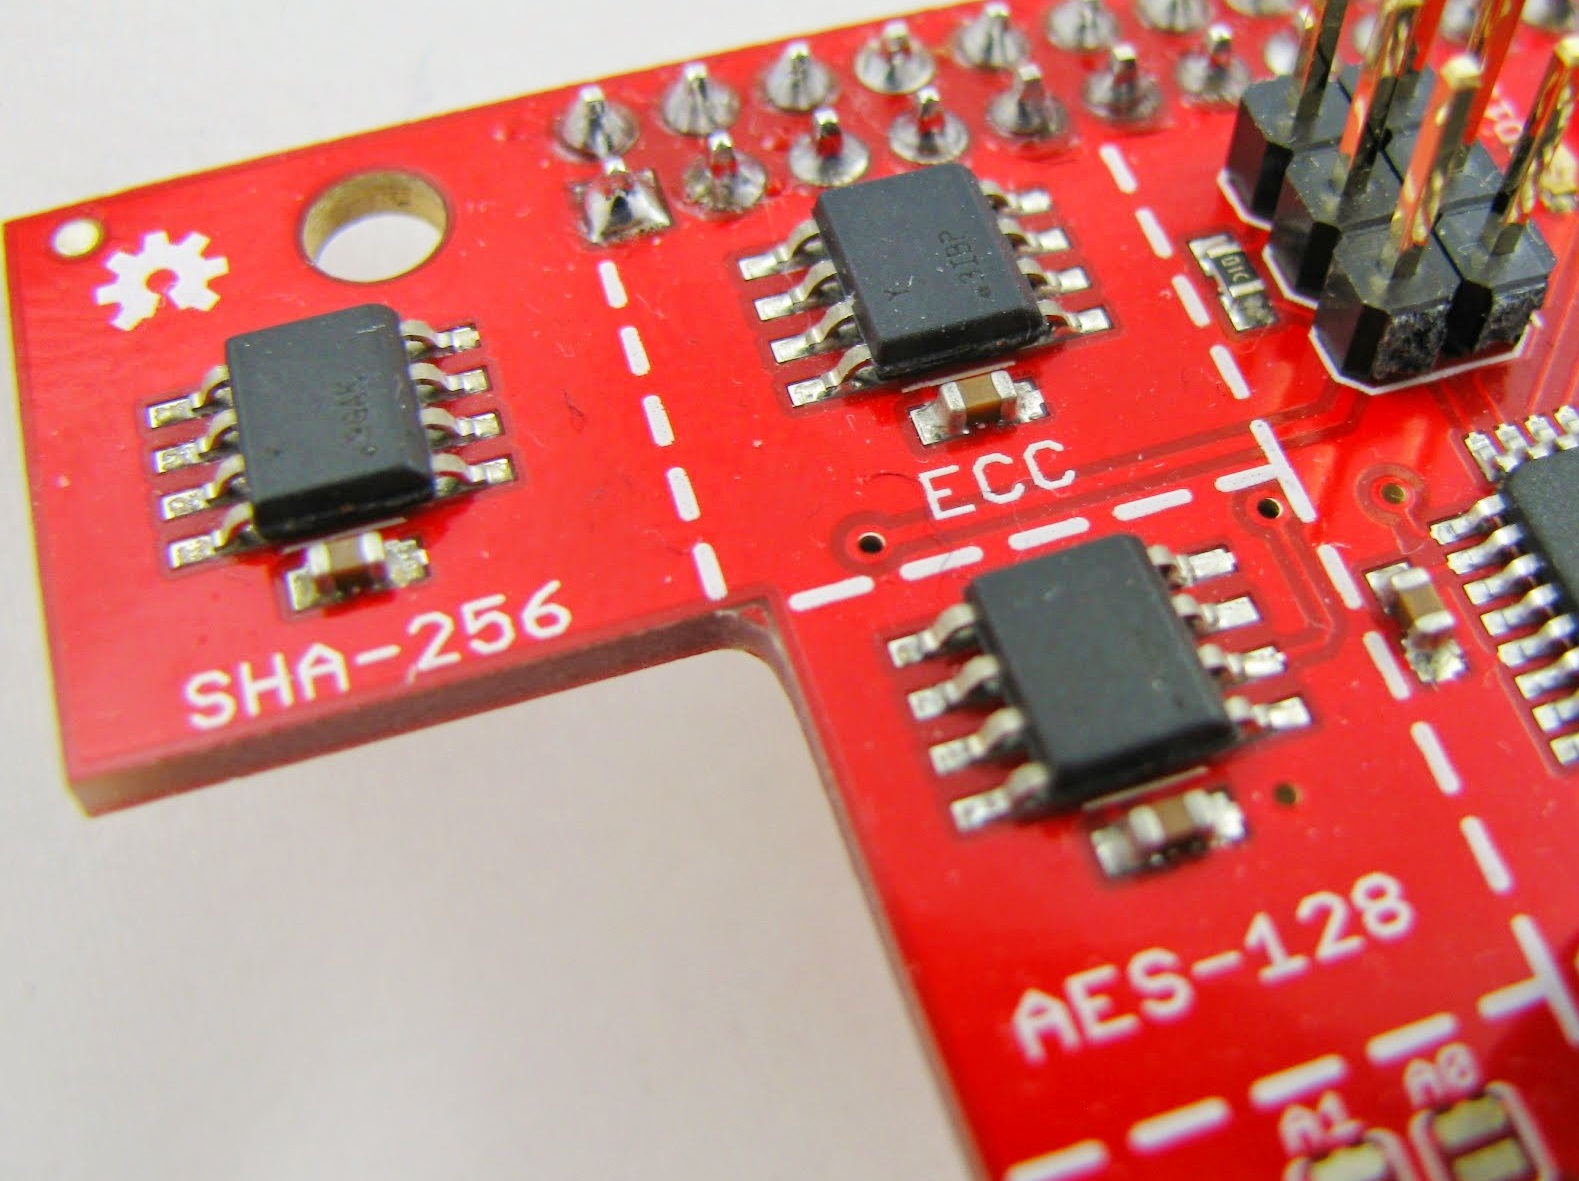
\includegraphics[width=0.9\linewidth]{gfx/atmel} \\ Atmel's cryptography chips.}
offers a serial chip for secure key storage, AES128 execution and random number generation. Another serial chip like ESP8266 offers WiFi connectivity, typically used with Arduino, and can also perform AES encryption. For random number generation, a technique used with Contiki devices is to read from sensors aleatory data and use it as seed.

All these alternatives depend on the target device, but are all valid, and would substitute OpenSSL with only a Serial communication library, so we can talk to the dedicated chips.

\hfil

The \textit{interfaces} and \textit{external utilities} sections  allow that the project is easily ported to specific targets without modifying the smart card logic.



\subsubsection{Execution workflow}

The sequence diagram from \autoref{fig:sequenceBIOSC} shows the execution of the PoC IoT smart card.



\begin{figure}[bth]
	\begin{center}
		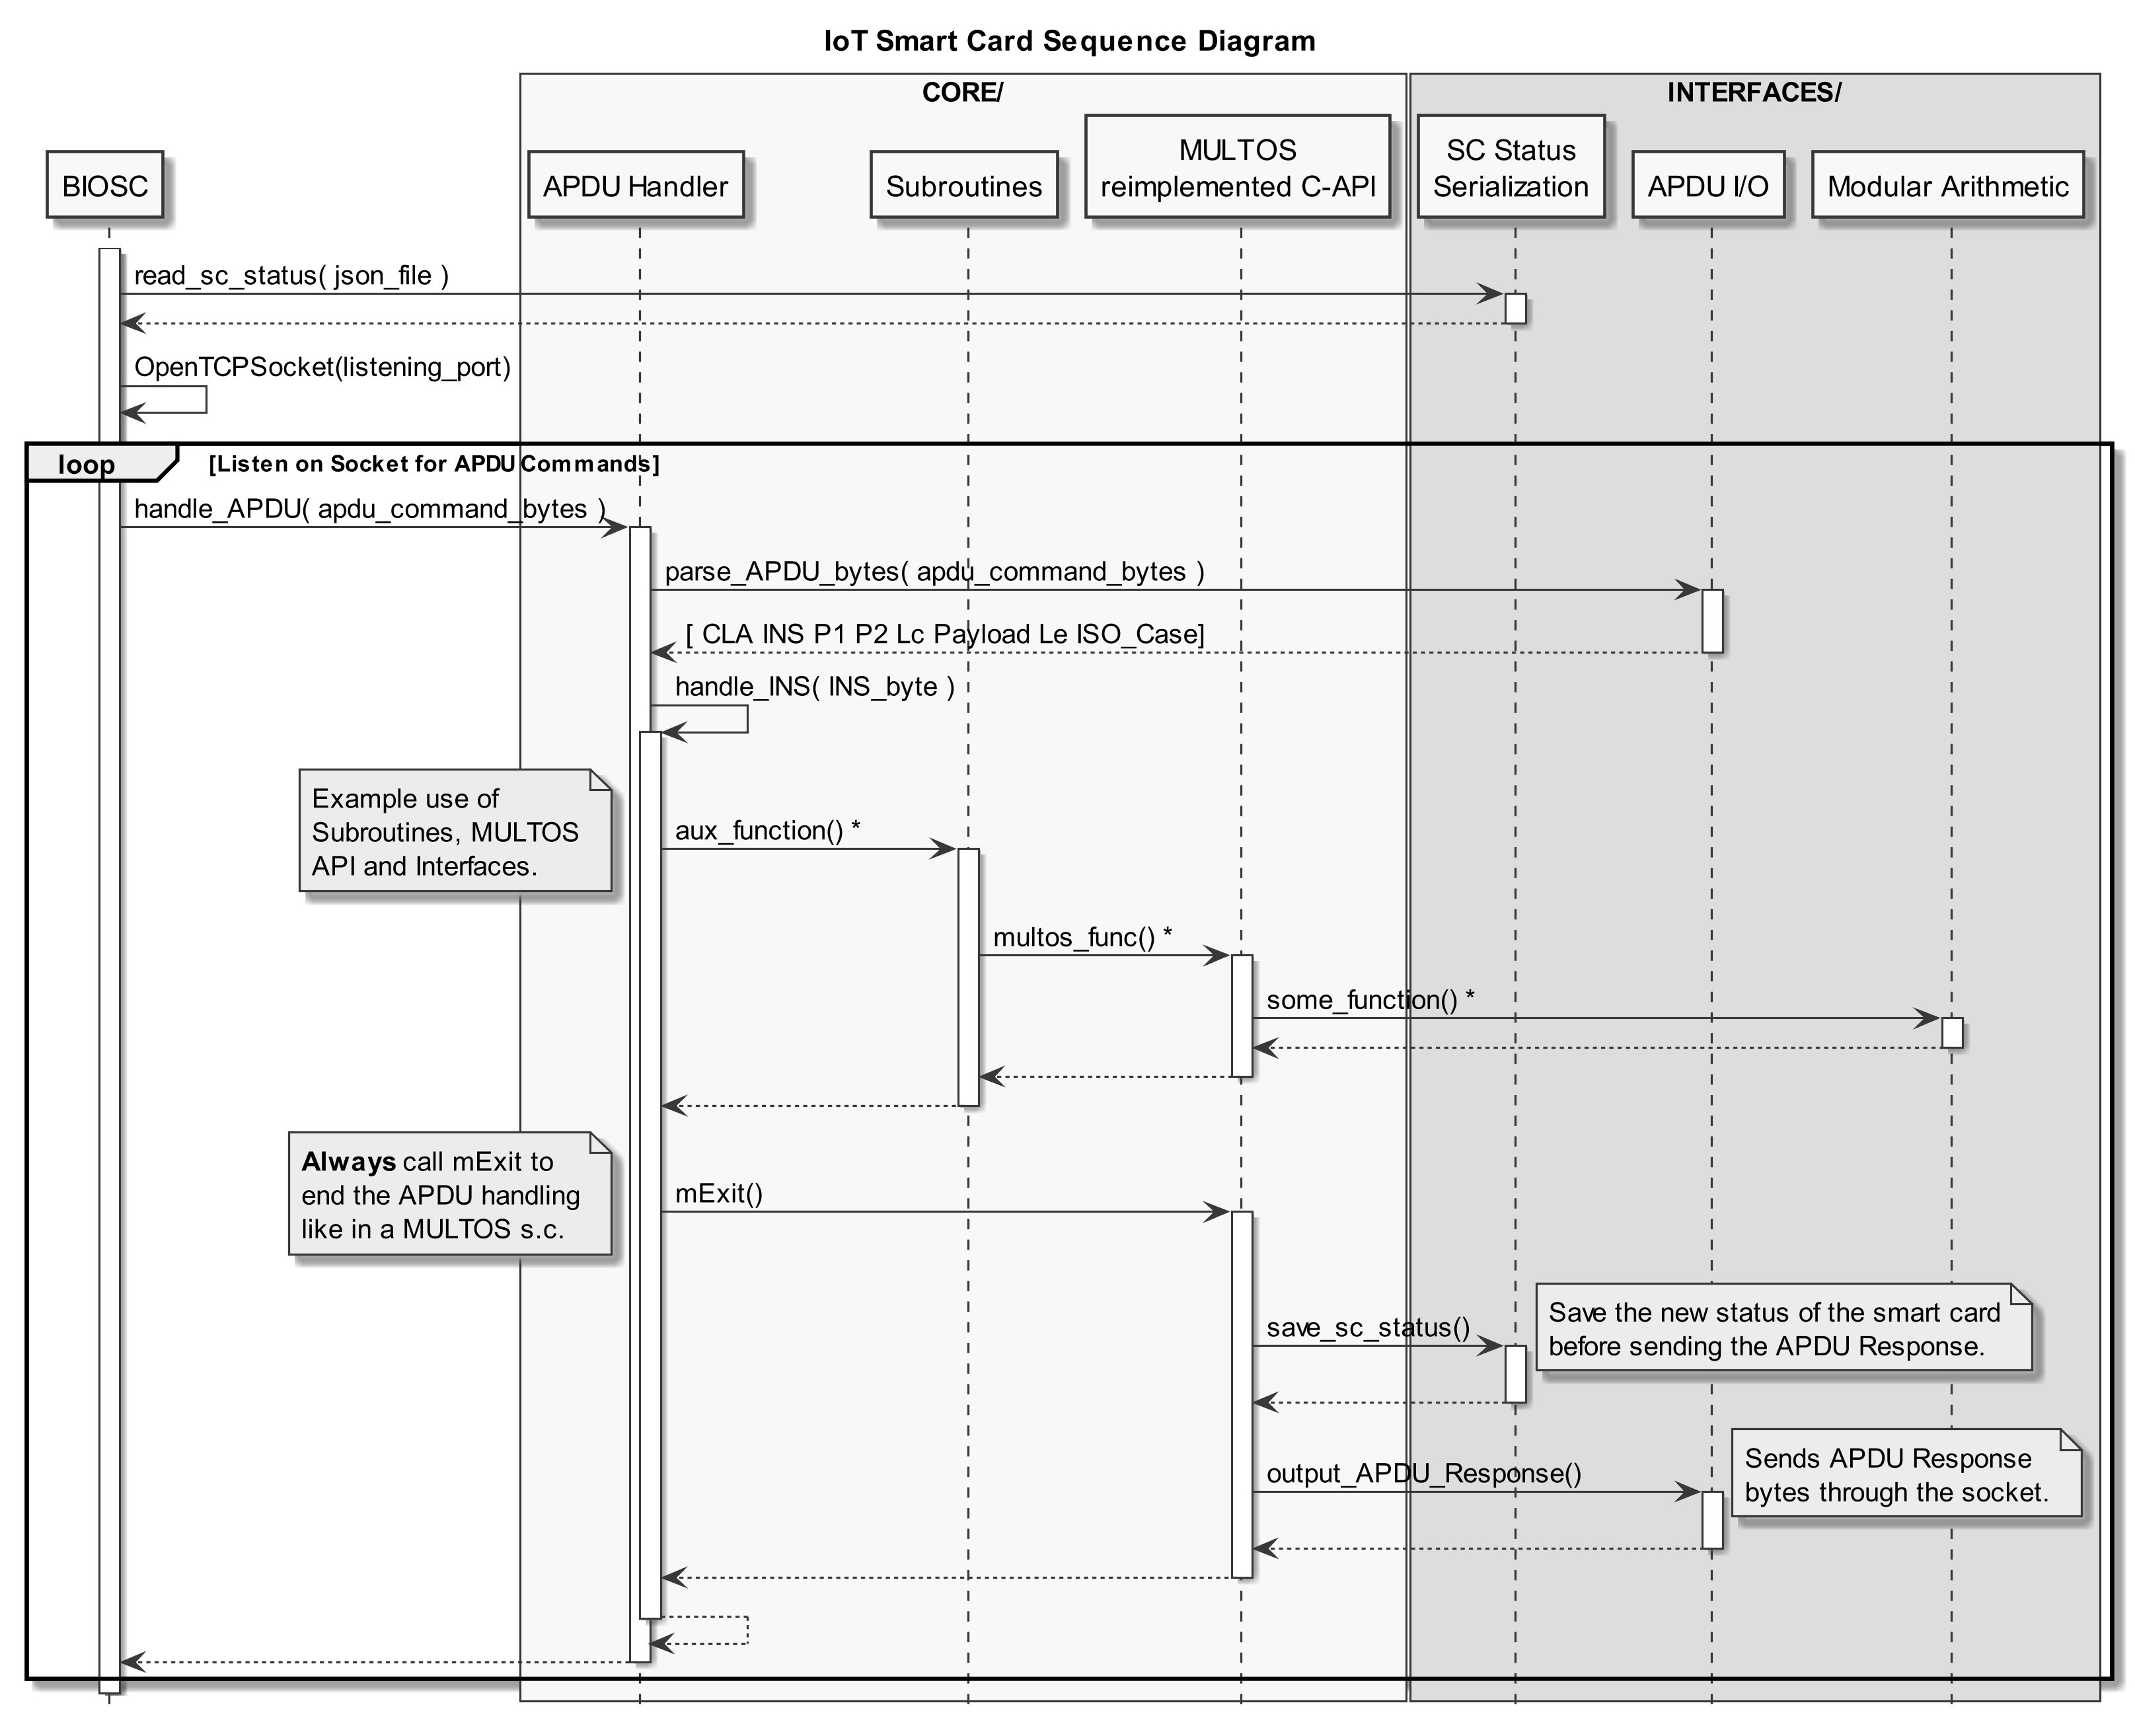
\includegraphics[width=\linewidth]{gfx/UML/sequenceBIOSC}
	\end{center}
	\caption{IoT Smart Card Sequence Diagram.}
	\label{fig:sequenceBIOSC}
\end{figure}



The program starts with the \texttt{main} function in BIOSC, that deserializes the status from the Json file, and listens on a loop for APDU Commands from the delegation server.

Every time an APDU Command arrives, it calls the function \texttt{handle\_APDU()} with the raw APDU bytes. The Handler calls the APDU I/O interface to parse the bytes, storing in global variables the APDU structure. Using a \texttt{switch-case} expression on the \texttt{INS} byte, the Handler calls an \textit{Instruction handler} function.

Inside this function, it may call multiple functions from the Subroutines, that may call MULTOS C-API functions, Which in turn may use an interface to perform its functionality.


As we mentioned, every instruction handler must end, before the \texttt{return;} expression, with \texttt{mExit} or  \texttt{output\_large\_data()}, that will use \texttt{mExit}. This reimplemented MULTOS function will save the current status of the smart card, with the help of the serialization interface, and once the file is saved, it outputs the APDU Response back to the delegation server.

After returning from \texttt{mExit}, the instruction handler and the APDU handler functions, the program listens again from the socket, until an $0xff$ byte is received.









%\include{multiToC} % <--- just debug stuff, ignore for your documents
%************************************************
\chapter{Validation and Performance Evaluation}\label{ch:validation}
%************************************************

In this chapter, we will describe the deployment of three testing scenarios: a laptop, a Raspberry Pi 3, and a Omega2 IoT device with the Raspberry Pi 3 as the delegation server. We will measure and compare the results to determine if the proposed solution is feasible or must be submitted to revision.

\section{Testbed description}

First, we shall describe the example Attribute Based Credential system in use. Then, the hardware we will use in our benchmarking.

\subsection{P2ABCE setting}

To test the correct execution of the \textit{IoT smart card}, we will use the ABC system from the tutorial in the P2ABCE Wiki \citep{p2abcurlwiki}. It is based on a soccer club, which wishes to issue VIP-tickets for a match. The VIP-member number in the ticket is inspectable for a lottery, ie. after the game, a random presentation token is inspected and the winning member is notified.

First the various entities are \textbf{setup}, where several artifacts are generated and distributed. Then a ticket credential containing the following attributes is issued:

\begin{verbatim}
First name: John
Last name: Dow
Birthday: 1985-05-05Z
Member number: 23784638726
Matchday: 2013-08-07Z
\end{verbatim}

During \textbf{issuance}, a \textit{scope exclusive pseudonym} is established and the newly issued credential is bound to this pseudonym. This ensures that the ticket credential can not be used without the smart card.

Then \textbf{presentation} is performed. The \textit{presentation policy} specifies that the member number is inspectable and a predicate ensures that the matchday is in fact $2013-08-07Z$. This last part ensures that a ticket issued for another match can not be used.

The ticket holder was lucky and his presentation token was chosen in the lottery. The presentation token is therefore inspected.


\hfil

\subsection{Execution environment}

First we will execute the test in our development machine (laptop). After asserting that the services work as expected, we then run the test in a Raspberry Pi 3, exactly like in the laptop. Finally, we will deploy the IoT smart card in a Omega2 and the delegation services in the Raspberry Pi 3. After every test, we checked that the issuing and proving were successful, in case a cryptographic error appeared in the implementation. 

Lets have a closer look at the hardware of each device:


\paragraph{Development laptop}\marginpar{
	\vskip0pt
	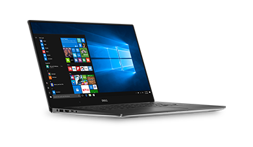
\includegraphics[width=0.8\linewidth]{gfx/DELL}
	
	DELL XPS 15
}
Our device is a DELL XPS 15, with a Core i7-6700HQ at 3.5GHz quad core processor and 32GB of DDR4 RAM, running Ubuntu 16.10.

This is a powerful machine that can simulate the performance of many servers and clients that would implement P2ABCE in a real environment, giving a reference point for performance comparisons.

\paragraph{Raspberry Pi 3}\marginpar{
	\vskip0pt
	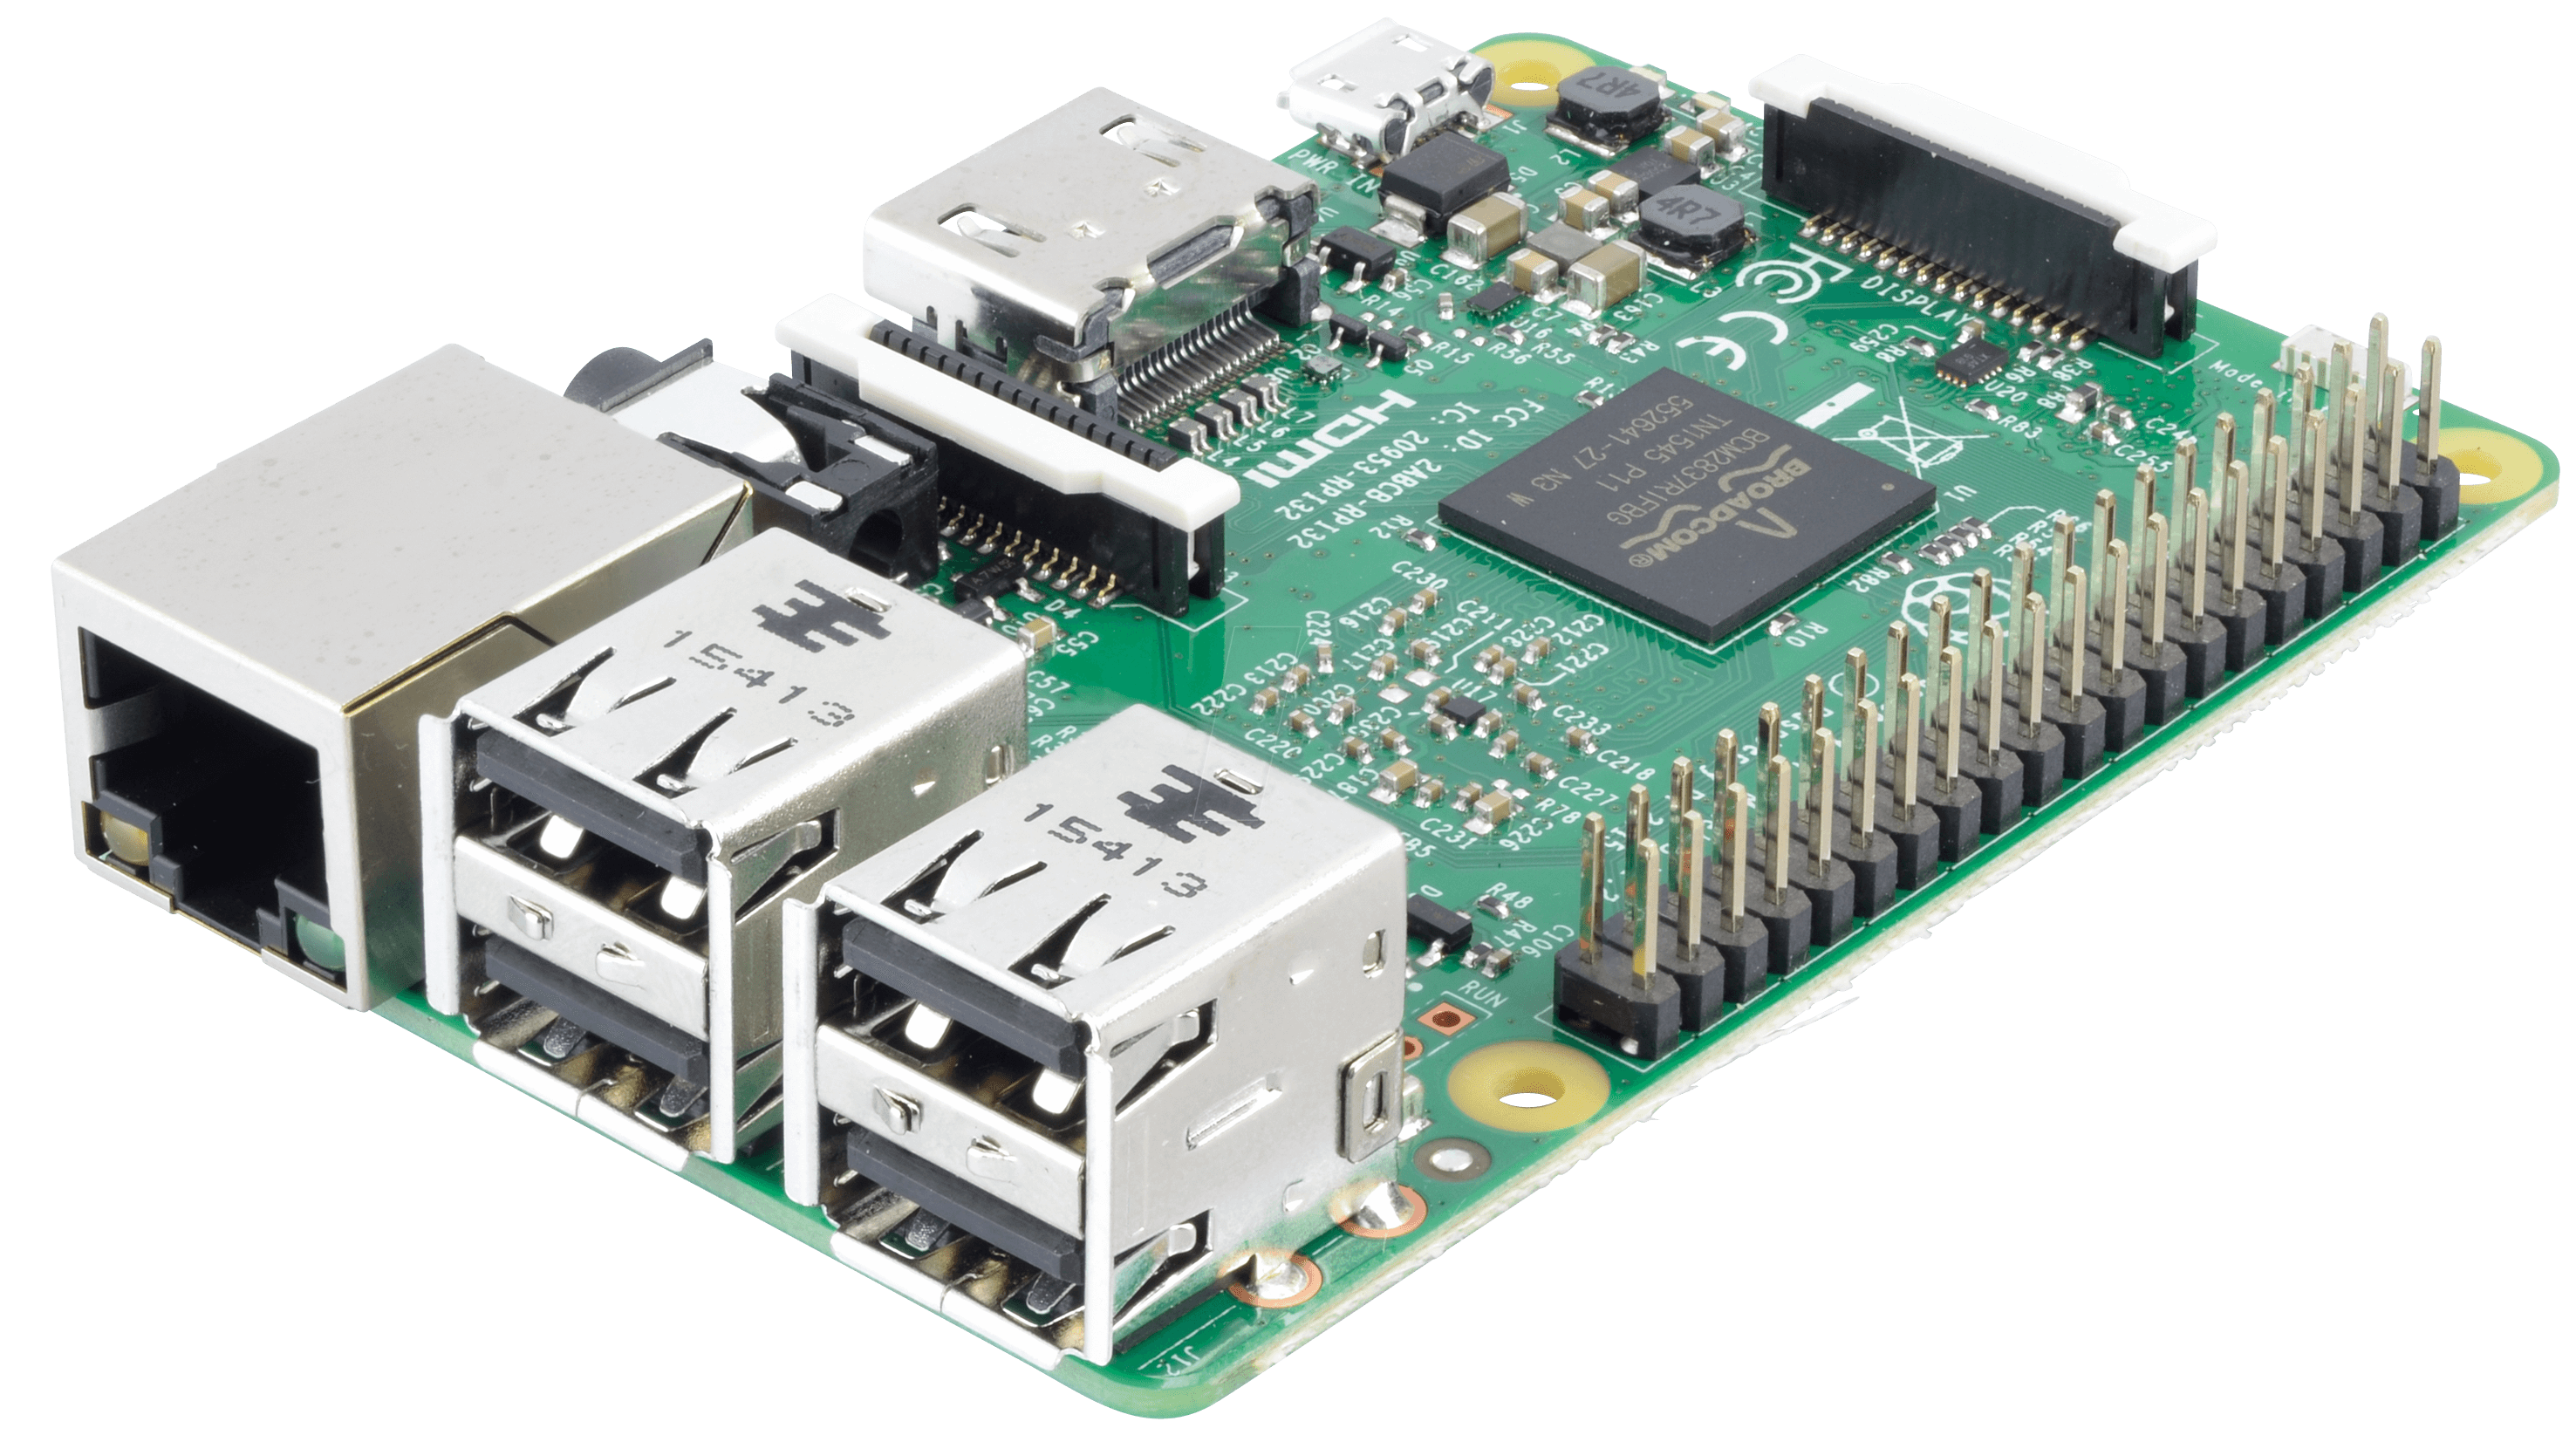
\includegraphics[width=0.8\linewidth]{gfx/RPi3}
	
	Raspberry Pi 3
} A familiar environment, powerful enough to debug and hold the delegated P2ABCE Java services of P2ABCE with its 1GB of RAM, and with two network interfaces, perfect to work as the gateway for the IoT devices to the Internet.

Only a microSD with enough space to burn the OS is needed to plug\&play with the Raspberry Pi. We use Raspbian, a stable Debian based distro, recommended by the Raspberry Pi designers, and ready to use with the P2ABCE compiled \textit{self-contained .jar} services.

\begin{table}[h]
	\myfloatalign
	\begin{tabularx}{0.75\textwidth}{ll} \toprule
		CPU & ARMv8 64bit quad-core @1.2GHz \\
		RAM & 1GB \\
		Storage & microSD \\
		Firmware & Raspbian (Debian based distro) \\
		Connectivity & Wifi n + Ethernet \\
		Power & 5V 2A \\
		\bottomrule
	\end{tabularx}
	\caption[Raspberry Pi 3 Specifications]{Raspberry Pi 3 Specifications.}
	\label{tab:RPi3Specs}
\end{table}


\paragraph{Onion Omega2}\marginpar{
	\vskip0pt
	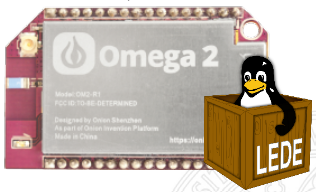
\includegraphics[width=\linewidth]{gfx/Omega2}
	
	Onion Omega2
} A device that falls inside the category of IoT, powerful enough to run a Linux environment, LEDE, where we can develop and debug the first PoC without troubling ourselves with problems not related to the project itself.


\begin{table}[h]
	\myfloatalign
	\begin{tabularx}{0.75\textwidth}{ll} \toprule
		MCU & Mediatek MT688 \citep{MT7688} \\
		CPU & MIPS32 24KEc 580MHz \\
		RAM & 64MB \\
		Storage & 16MB \\
		Firmware & LEDE (OpenWRT fork distro) \\
		Connectivity & Wifi b/g/n \\
		Power & 3.3V 300mA \\
		\bottomrule
	\end{tabularx}
	\caption[Onion Omega 2 Specifications]{Onion Omega2 Specifications.}
	\label{tab:Omega2Specs}
\end{table}



Nonetheless, the Omega2 needs fine tunning to start operating, and basic knowledge of electronics to make it work. The two main things to begin with Omega2 are:
\begin{itemize}
	\item A reliable 3.3V with a maximum of 800mA power supply, e.g. a USB2.0 with a step-down circuit, with quality soldering and wires to avoid unwanted resistances. The Omega2 will usually use up to 350mA, when the WiFi module is booting up. The mean consumption is about 200mA.
	\item A Serial to USB adapter wired to the TX and RX UART pins to use the Serial Terminal, to avoid the use of SSH over WiFi.
\end{itemize}


Also, we will need a cross-compiler to generate the smart card binary. Because we will use GMP and OpenSSL as shared libraries, the best option is to use the LEDE SDK. The SDK manages the available packages and generates the GCC toolchain. Also, using CMake, 
%TODO


\paragraph{The network} In our third scenario, the Raspberry Pi 3 and the Omega2 will talk to each other over TCP. This implies possible network delays depending on the quality of the connection. The Raspberry Pi 3 is connected over Ethernet to a switch with WiFi access point. The Omega2 is connected over WiFi n to said AP. To ensure the delay wasn't significant, we measured 6000 APDU messages, and the results show that the mean transmission time is less than half a millisecond per APDU. As we will see in the results section, this network time is negligible.

\paragraph{Future work for tests} The lack of a physical MULTOS smart card precludes us to load and test the ABC4Trust Card Lite's code and measure the time P2ABCE would need when using the \textit{HardwareSmartcard} class. This would be really interesting because for a single method from the \textit{Smartcard} interface, \textit{HardwareSmartcard} implementation needs to send multiple APDU Commands, but \textit{SoftwareSmartcard} can perform the operations immediately, with the full computer's resources.




\section{The test code}

In this section we present the scripts and binaries used during the tests.

There are three pieces of software that conform the test: the P2ABCE services, the IoT smart card, and shell scripts automatizing the REST calls, from the terminal.

\paragraph{P2ABCE services}\hfil

This is a common part to our three sets. The services are compiled in a self-contained Jetty web server, or in WAR format, ready to be deployed in a server like Tomcat. We use the same JAR files with the embedded Jetty web server for the PC and Raspberry Pi.

We modified the User Service code to measure the execution elapsed time for each REST method. We don't measure the time the web server spends processing the HTTP protocol and deciding which Java method to call.


\paragraph{IoT smart card}\hfil

Our C implementation of the P2ABCE smart card, compiled for the Omega2, with BIOSC listening on port 8888 for the APDU messages.

We tested the execution in two modes, a full logging where every step was printed in terminal, and another one with no logging. With the first mode, we can check a proper execution, every byte exchanged, and with the second one, we measure the execution without unnecessary I/O.

\paragraph{Shell script} \hfil

To orchestrate all the services we use a simple script that performs the REST calls using  \textit{curl}. Here we perform the mentioned steps: setup of the P2ABCE system, issuance of the credential and a prove for the presentation policy.

In the setup, the system parameters are generated, indicating key sizes of 1024 bits, the ones currently supported by the ABC4Trust and IoT smart cards. Then the system parameters and public keys from the services (issuer, inspector, revocation authority) are also exchanged.

In the issuance, a two step protocol is performed by the User. The Issuer and the User send each other the XML data with the cryptographic information, and finish the protocol with a credential issued inside a smart card, software (Java) or hardware (physical or IoT).

Finally, a Verifier sends the User a \textit{presentation policy}. The User generates a \textit{presentation token} for the Verifier and Inspector.


%%%%%
There are two script versions, one where every REST call is done from the same machine, therefore avoiding the exchange of the XML files by other means (like \textit{scp}); the other one is ready to be executed on a real setup, two scripts, one for the Omega2, where the REST calls are the delegation on the Raspberry Pi 3, and other for the PC, running the Issuer and Verifier as third party entities. The XML files generated by each service can be sent with the same protocol the IoT device and the Verifier, for example, would communicate in the real world. This way it's clearer that the \textit{curl} commands are the delegation protocol for the IoT device, and then the IoT device can send the XML as it wishes, over the Internet, Bluetooth, NFC, etc.
%%%%%


\section{Results}

After 20 executions for each scenario (laptop, RPi3, Omega2+RPi3), we take the means and compare each step of the testbed.

It is worth noting that during the test, the measured use of the CPU showed that P2ABCE does not benefit of parallelization, therefore, it only uses one of the four cores in the laptop and Raspberry Pi 3.

To test the network, we sent six thousand APDUs to the Omega2, but instead of calling the \textit{APDU handler}, the Omega2 responded with the same bytes back. This way, the Omega2 only performed the simple BIOSC protocol, reading from and writing to the TCP socket.
The APDUs had multiple sizes, taken from the most common APDUs logged in during a successful execution. The test showed that our network speed was around $0.014$ ms per byte.


\paragraph{The setup}\hfil

The first step of our testbed. The Omega2 doesn't intervene until the creation of the smart card, therefore, the times measured in the second and third scenarios are practically identical.

\begin{figure}[bth]
	\myfloatalign
	\subfloat[Times and relative speedup]
	{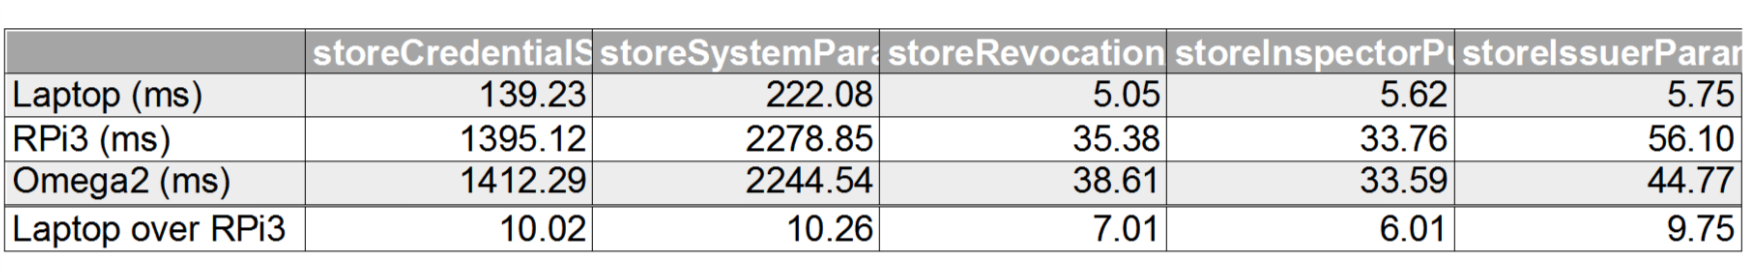
\includegraphics[width=\linewidth]{gfx/graphics/setuptable}} \quad
	\subfloat[Comparison graph]
	{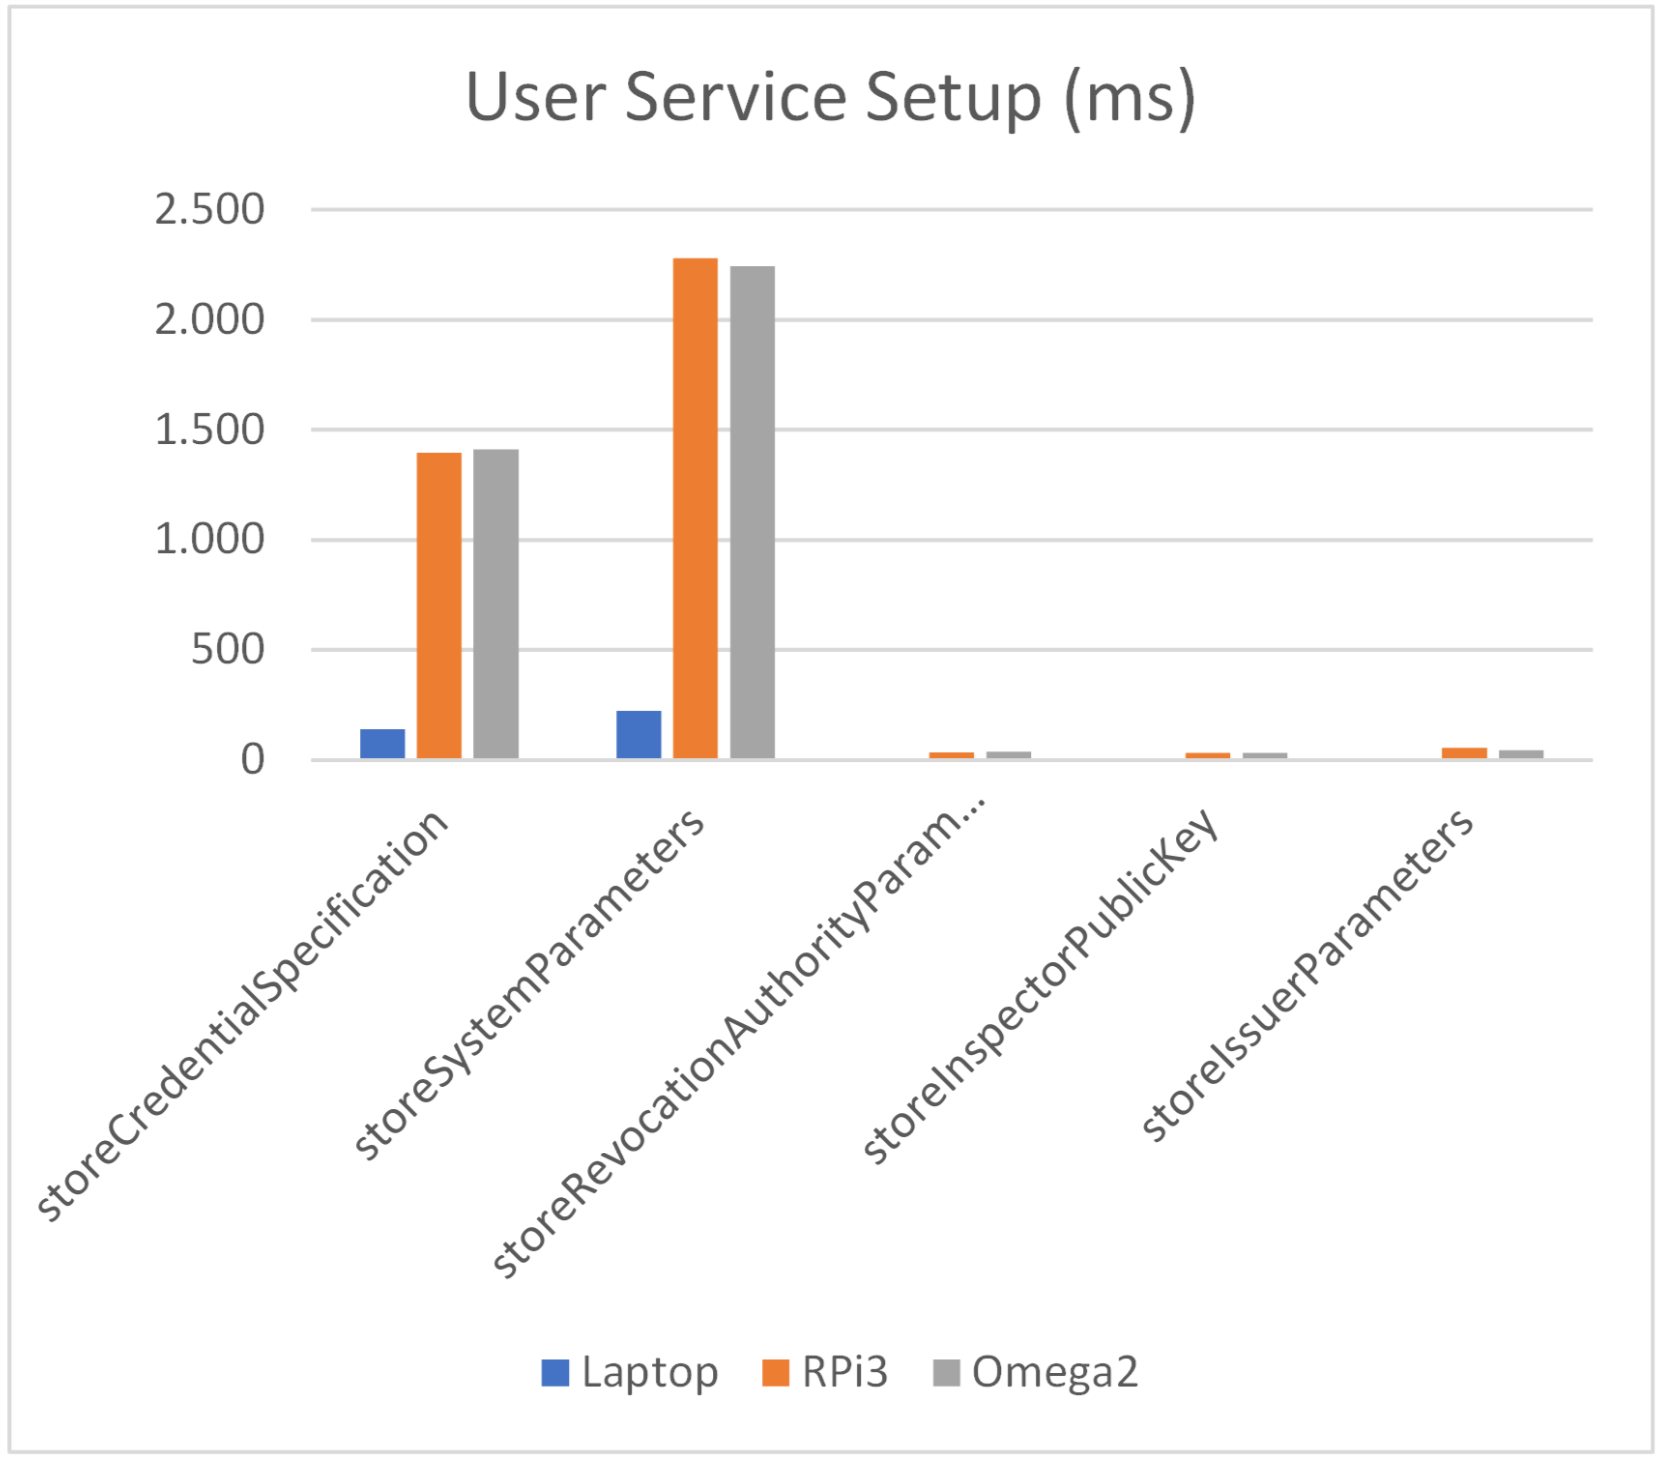
\includegraphics[width=.8\linewidth]{gfx/graphics/setup}} \\
	\caption{Setup times (milliseconds)}
	\label{fig:setup:graph}
\end{figure}

As we can see in \autoref{fig:setup:graph}, the laptop is about ten times faster than Raspberry Pi 3, but considering that the highest time is less than two and a half seconds, and that the setup is done only once, this isn't a worrisome problem.

\paragraph{Creation of the smart card}\hfil

Here we create a \textit{SoftwareSmartcard} or a \textit{HardwareSmartcard} object that the User service will use in the following REST calls.

The REST method to create a \textit{SoftwareSmartcard} is $/createSmartcard$, and to create a \textit{HardwareSmartcard}, using the \textit{IoTsmartcardio} implementation, we use $/initIoTsmartcard$.


\begin{figure}[bth]
	\myfloatalign
	\subfloat[Times and relative speedup]
	{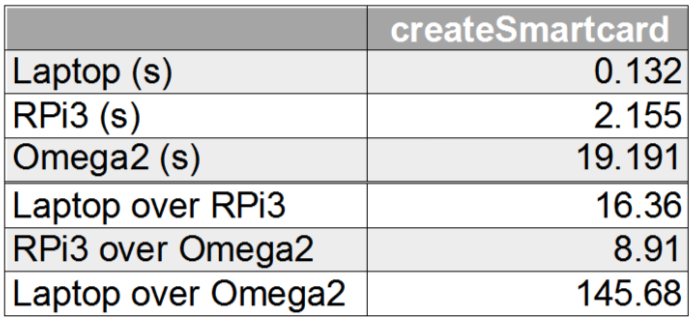
\includegraphics[width=0.5\linewidth]{gfx/graphics/createSCtable}} \quad
	\subfloat[Comparison graph]
	{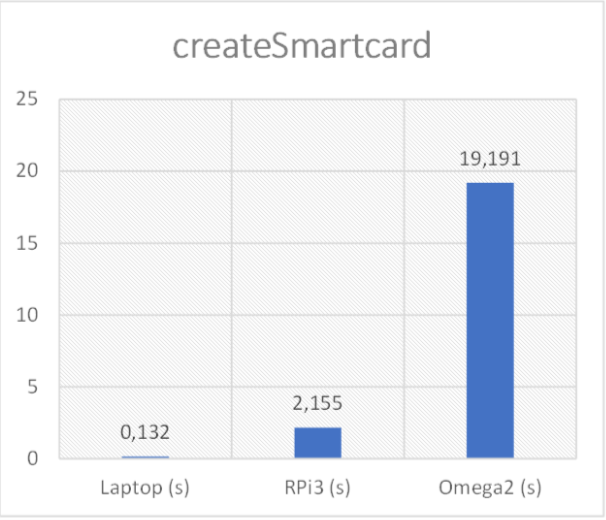
\includegraphics[width=0.45\linewidth]{gfx/graphics/createSC}} \\
	\caption{Create smart card times (seconds)}
	\label{fig:createSmartCard:graph}
\end{figure}

From \autoref{fig:createSmartCard:graph} we see that the RPi3 is about 16 times slower than the laptop in the creation of the \textit{SoftwareSmartcard}, but almost 9 times faster than the setup of the smart card in the Omega2 using APDUs. This gives us that the laptop is 145 times faster than the combination of RPi3 and Omega2 in our IoT deployment.
But looking at the times, this process lasts up to 20 seconds, making it something feasible.

Again, this operation is done only once per device, and includes commands from the creation of the PIN and PUK of the smart card, to storing the system parameters of P2ABCE, equivalent to the previous setup step.



This is the first interaction between the RPi3 and the IoT smart card running in the Omega2. To setup the smart card \textbf{30 APDU Commands}, and their respective Responses, are exchanged, as shown in \autoref{ch:resultsdiagrams}, \autoref{fig:APDUsInitIoTSC}, with a total of $1109$ bytes. From our network benchmark, using TCP sockets, the delay in the transmission is only around 15 and 20 ms, negligible, as we said, compared to the almost 20 seconds the operation lasts.


\paragraph{Issuing of the credential}\hfil

The issuance is done in three steps for the User service, shown in \autoref{fig:IssuanceInteraction} with a red note showing the start of each step for the User delegation, in green for the interactions between Issuer and User, and the darker red is the Identity service, choosing the first available identity to use. The arrows in the figure show the REST calls performed during the test, where the IoT device acts as User, the RPi3 hosts the P2ABCE delegation services and the laptop is the Issuer.

The three delegation steps and the REST method called are:

\begin{center}
	\begin{tabular}{l|l}
	First issuance protocol step & $/issuanceProtocolStep$ \\
	Second issuance protocol step  & $/issuanceProtocolStepUi$ \\
	\textit{(end of first step for the User)} & \\
	Third issuance protocol step & $/issuanceProtocolStep$ \\
	\textit{(second step for the User)}  & \\
\end{tabular}
\end{center}


\begin{figure}[bth]
	\begin{center}
		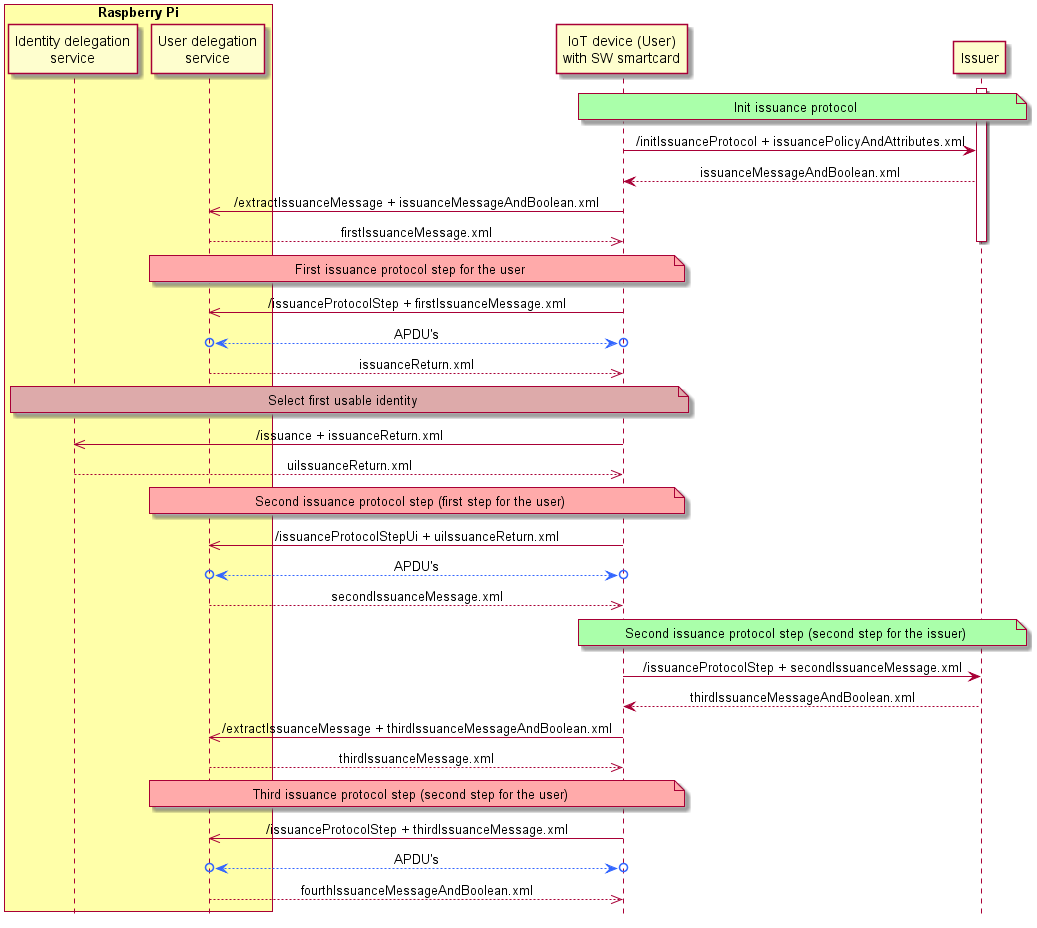
\includegraphics[width=\linewidth]{gfx/IssuanceInteraction}
	\end{center}
	\caption{Issuance interaction.}
	\label{fig:IssuanceInteraction}
\end{figure}



As we can see, the three REST calls to the delegation User service involve communication with the smart card. We show in \autoref{ch:resultsdiagrams}, \autoref{fig:IssuanceAPDUs}, the APDU Commands used for each REST call in the issuance.
There are 45 APDU Commands in total, $3197$ bytes exchanged, that would introduce a latency of 45ms in the network, negligible.


\begin{figure}[bth]
	\myfloatalign
	\subfloat[Times (ms) and relative speedup]
	{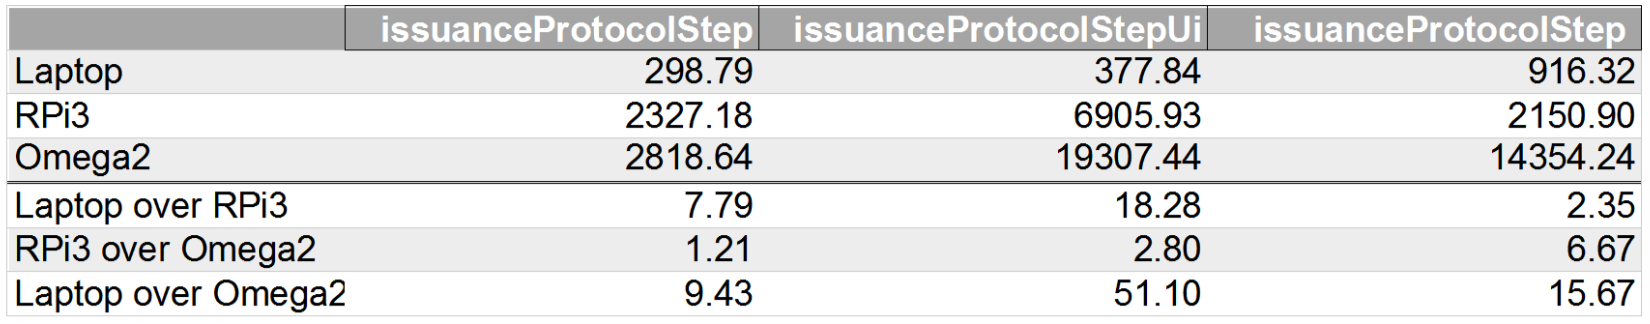
\includegraphics[width=\linewidth]{gfx/graphics/issuancetable}} \quad
	\subfloat[Comparison graph]
	{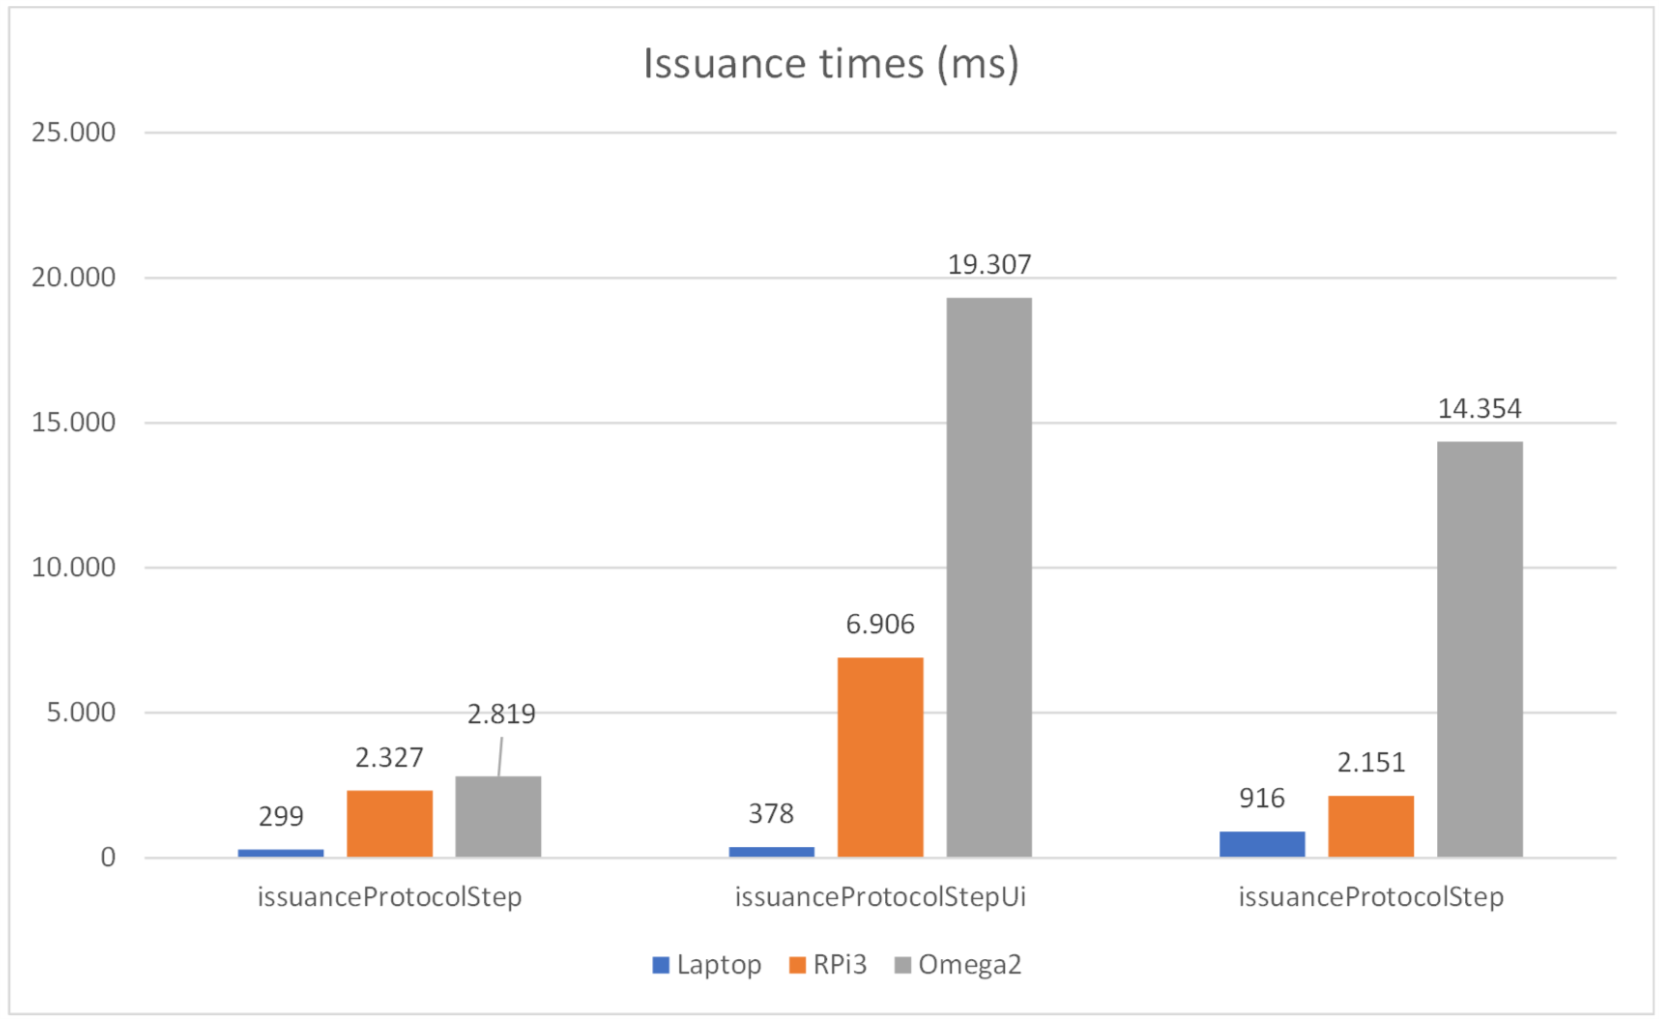
\includegraphics[width=.8\linewidth]{gfx/graphics/issuance}} \\
	\caption{Issuance times (milliseconds)}
	\label{fig:issuance:graph}
\end{figure}

In \autoref{fig:issuance:graph} we have the times spent in each REST call. The laptop shows again to be many times faster than the other two scenarios, but the times are again feasible even for the IoT environment.

Lets compare the Raspberry Pi 3 and the Omega2 executions. There is a correlation between the number of APDU Commands needed in each step with the increment in time when using the IoT smart card, that is, how much the delegation server.

The first one only involved one APDU, with $33$ bytes total (Command and Response), and times are almost identical. The second call needed $34$ APDUs, with $1623$ bytes, and the increase in time is around tree times slower than the RPi3 on its own. The third call used $20$ APDUs, $1541$ bytes, and makes the IoT scenario almost 7 times slower.

The analysis shows where there are more cryptographic operations involving the Omega2, and because the amount of data exchanged is minimal, the difference in processing power between Omega2 and Raspberry Pi 3 is clear.



\paragraph{Presentation token}\hfil

The final step of the test involves a Prove, or Presentation in P2ABCE, where the Verifier sends the User or Prover the Presentation Policy, and the User answers with the Presentation Token, without more steps. In \autoref{fig:ProvingInteraction}, using the same colors as in the Issuance interaction, we can see the delegation messages done by the Omega2.

To ensure that all the process was successful, it's enough to check if the Verifier and the Inspector returned XML files, accepting the prove, or an error code. Of course, every execution measured in the test was successful.

In \autoref{ch:resultsdiagrams}, \autoref{fig:APDUsProving}, we provide the APDU Commands for each step, $28$ in total, with $1939$ bytes, giving us about $27$ms of delay in the network transmission.



\begin{figure}[bth]
	\begin{center}
		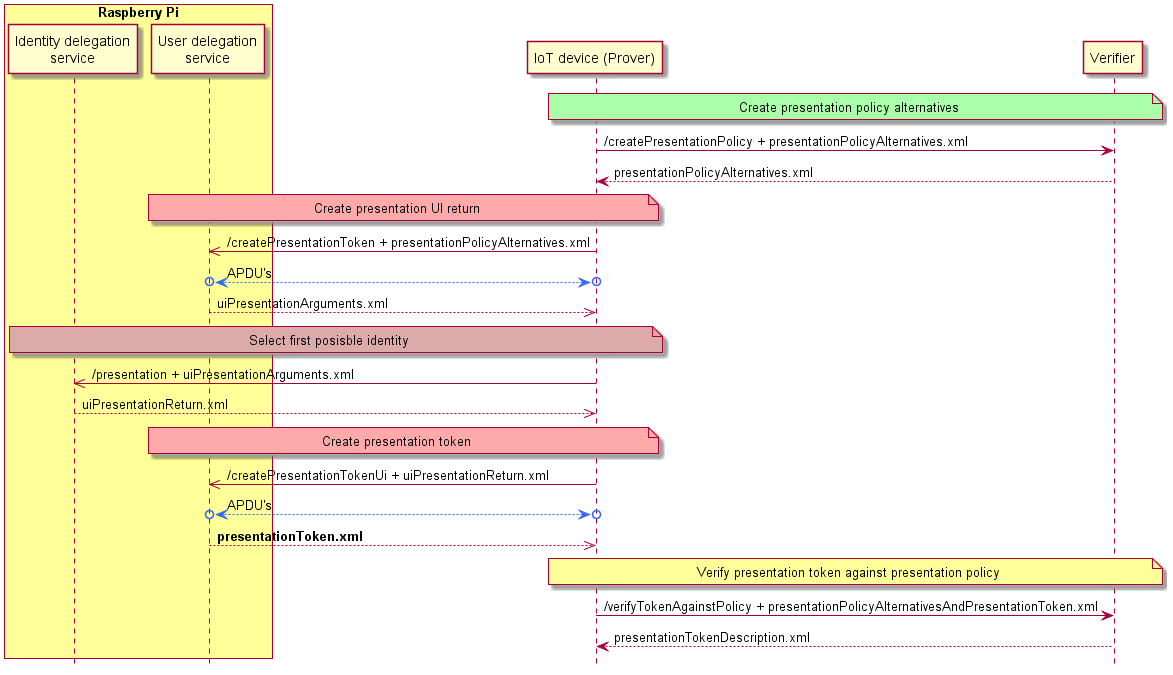
\includegraphics[width=\linewidth]{gfx/ProvingInteraction}
	\end{center}
	\caption{Proving interaction.}
	\label{fig:ProvingInteraction}
\end{figure}



Again, as shown in \autoref{fig:proving:graph}, there is a correlation between the number of APDU Commands used, the work the IoT smart card must perform, and the time measured. The $20$ APDU Commands in the first call make the IoT deployment almost $8$ times slower than the Raspberry Pi 3; but with only $8$ APDU Commands, the second one is less than $1.5$ times slower.

Nonetheless, it's significant the difference in performance between the laptop and the Raspberry Pi 3 in the last REST call, more than $40$ times slower, even using the \textit{SoftwareSmartcard}.


\begin{figure}[bth]
	\myfloatalign
	\subfloat[Times (ms) and relative speedup]
	{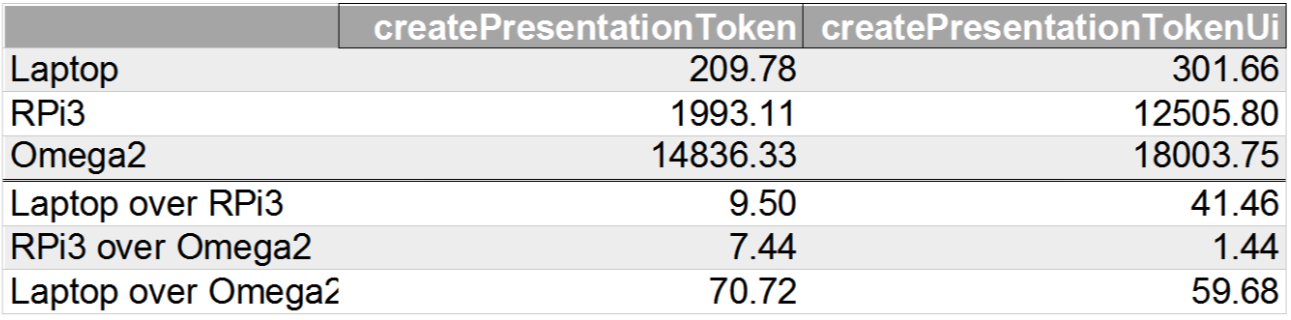
\includegraphics[width=.8\linewidth]{gfx/graphics/provingtable}} \quad
	\subfloat[Comparison graph]
	{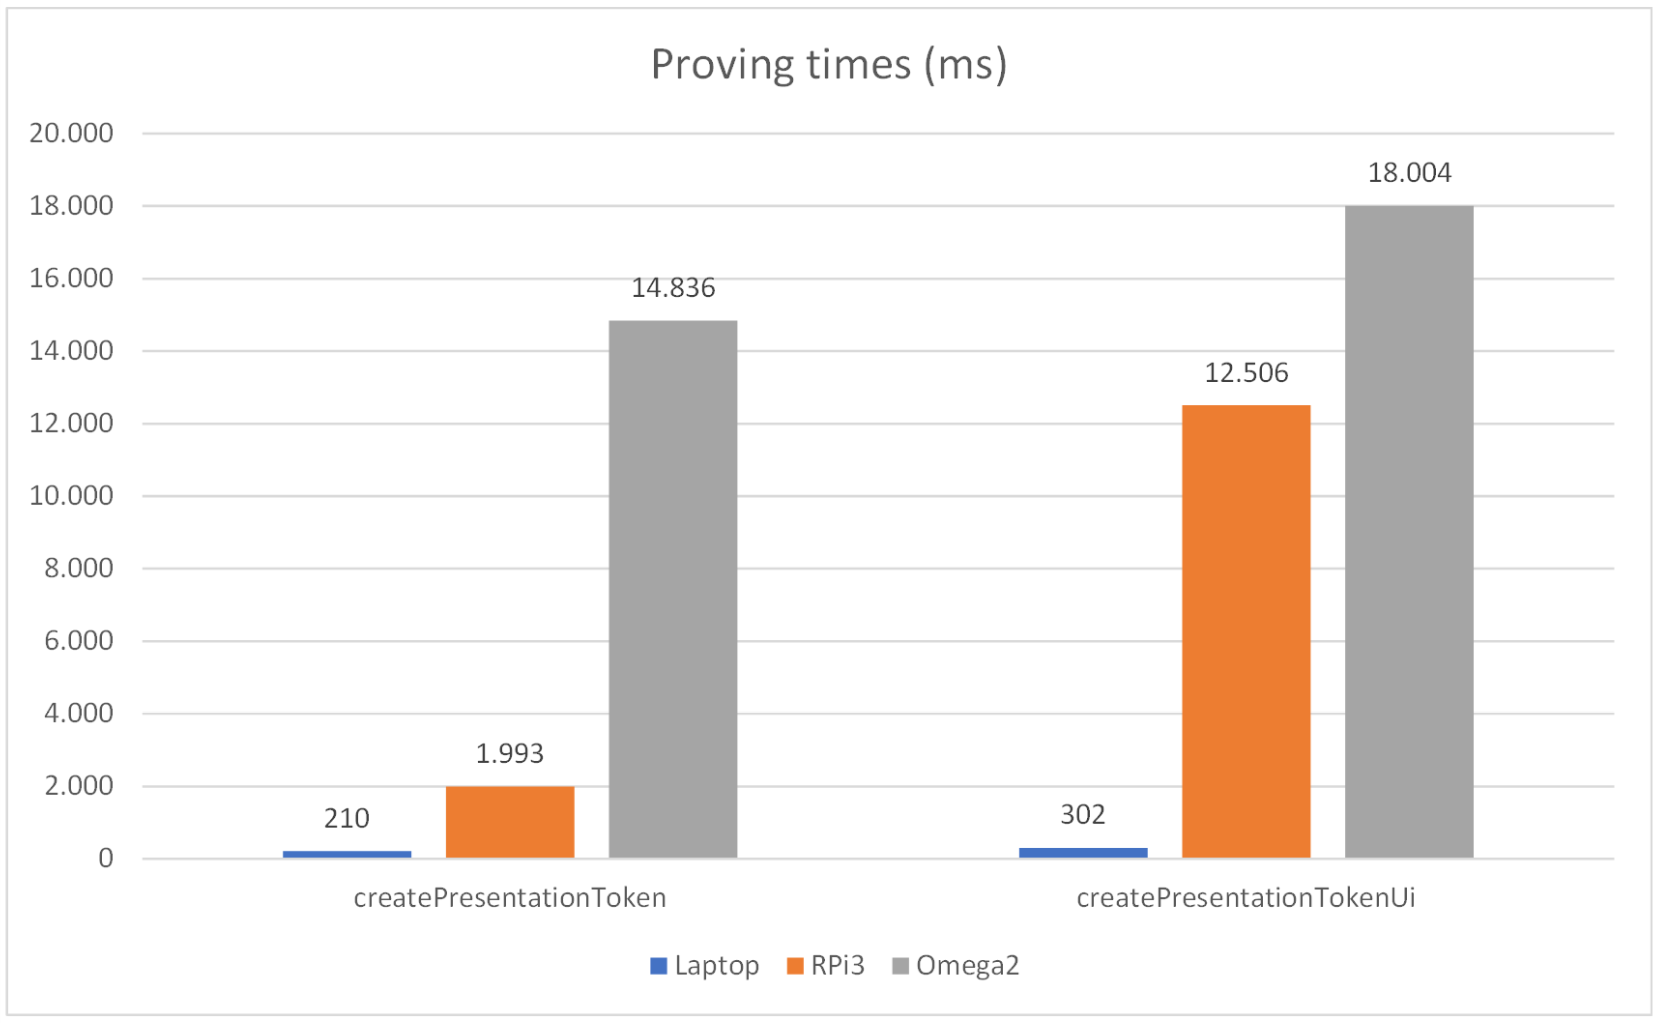
\includegraphics[width=.7\linewidth]{gfx/graphics/proving}} \\
	\caption{Proving times (milliseconds)}
	\label{fig:proving:graph}
\end{figure}

Unlike the previous steps, the Presentation or Proving is done more than once, being the key feature of ZKP protocols. The laptop performs a prove in less than one second, the RPi3 needs $15$ seconds, but our P2ABCE IoT deployment needs $15$ seconds for the first step, and $18$s for the second step, $33$ seconds total to generate a Presentation Token.




\hfil

\paragraph{Memory usage on the Omega2}\hfil

Using the tool \textit{time -v} we can get a lot of useful information about a program, once it finishes. In our case, the binary with BIOSC and the smart card logic starts as an empty smart card, goes through the described process, and then we can stop it, as the User Service won't use it anymore.

After another round of tests, now using \textit{time -v}, the field named \textit{Maximum resident set size (kbytes)} shows the \textbf{maximum} size of RAM used by the process since its launch. In our case, this involves the use of static memory for the \textit{global variables} of the smart card logic, and the dynamic memory used by the third party libraries, like GMPlib, OpenSSL and cJSON.

GMP and OpenSSL always allocate the data in their own ADT, what involves copying the arrays of bytes representing the big modular integers from the cryptographic operations. cJSON, used in the serialization of the smart card for storage, and debug being human readable, stores a copy of every saved variable in the JSON tree structure, then creates a string (array of char) with the JSON, that the user can write to a file.

Understanding the many bad uses of memory done in this PoC is important for future improvements and ports. A custom modular library using the same array of bytes that the smart card logic, a binary serialization, and many improvements, are our future work.

With all that said, the mean of the maximum memory usage measured is $6569.6$ kbytes. Compared to the $64$MB of RAM available in the Omega2, our PoC could be executed in more constrained devices, given the system is compatible.





























%%%%%%%%%%%%%%%%%%%%%%%


% Consideraciones futuras: implementar directamente Smartcard interface vs seguir usando APDUs:  minimizan uso de red, facilitan protocolo de comunicación de las APDUs, son estándar, mejoran el mantenimiento del código: P2ABCE puede cambiar las interfaces, pero mantendrá compatibilidad con las smartcards, si implementamos Smartcard.java por cada cambio en la interfaz deberemos actualizar cada IoT smart card.

%************************************************
\chapter{Conclusions and Future Work}\label{ch:conclusions}
%************************************************

To finish this document, we sum up some conclusions from the work done, and results 
obtained. We will also enumerate some future lines of research that could start from
the work done in this project.

\section{Conclusions}

% Resultados son válidos: feseability, problema de tiempo en sistemas de tiempo real
% Se han conseguido objetivos planteados
% Experiencia: qué era más tedioso, dificultades durante diseño y desarrollo
% Primera aproximación de este tipo ~~: más bien somos el future work de...
% Aplicación de procedimientos aprendidos/aplicados durante el TFG/carrera
% ^ Novelty

The designed solution for the integration of Idemix and the Internet of Things provides new possibilities for the IoT security field, mainly in those scenarios where people's data is more vulnerable. However, there is a long path of research before we can see this in production. Many decisions depend on the specific deployment in course, and our solution tries to ease the best it all that future process.

With regards to the designed architecture, the flexibility of the Computation Offloading technique, identifying the key operations that can't be delegated, and those ones that can, allows us to define a general solution for the vast world of the Internet of Things. The IoT devices can operate as individual actors in the Idemix ecosystem. When in need of performing offloading, the delegation server also falls into the IoT class of devices, a great benefit for any real project, having as many options as possible, the solution delivered can be adapted to most of requirements. Nevertheless, being so open to any solution leaves us with a lot of work to do, researching what are the best options, comparing benefits and drawbacks.

Our PoC implementation demonstrates that this project is actually feasible, not by performing a simulation of an IoT device, like in \citep{vanet}. During its development, we had to investigate a lot of concepts related to IoT, smart cards, and even the insides of P2ABCE's code, to fix many existing bugs in the original project and minimize the amount of changes it had to undergo, in order to work with the IoT devices. 


\section{Future work}

% Mejoras PoC
% Mejoras arquitectura: estudiar entornos típicos IoT y definir un despliegue realista usando esta cryptografía
% De \citep{vullers2013efficient} tomar el código de Multos para Idemix "puro". De mi trabajo tomar la adaptación de una tarjeta MULTOS a código de máquina genérica. Perdemos soporte P2ABCE, pero siendo Idemix solo más eficiente.

%************************************************
\chapter{Draft}\label{ch:draft}
%************************************************


% TODO
% From Idemix To P2ABCE: reasons

\section{Smart card APDU}

To communicate the smart cards and the reader an standardized protocol is specified in ISO/IEC 7816-4 \citep{APDUISO}.

The messages, also kown as \ac{APDU}, are divided in APDU Commands and APDU Responses.

\textbf{APDU Commands} consist in 4 mandatory bytes (CLA, INS, P1, P2), and an optional payload.

\begin{itemize}
	\item CLA byte: Instruction class. Denotes if the command is interindustry standard or proprietary.
	\item INS byte: Instruction code. Indicates the specific command.
	\item P1, P2 bytes: Instruction parameters.
	\item Lc, 0-3 bytes: Command data length.
	\item Command data: Lc bytes of data.
	\item Le, 0-3 bytes: Expected response data length.
\end{itemize}

This way, minimal number of bytes are needed to transmit commands to the smart card, allowing manufacturer's personalization of the smart card behavior and capabilities along with standard operations.

\begin{figure}[bth]
	\begin{center}
		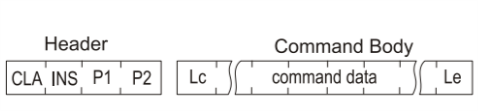
\includegraphics[width=0.55\linewidth]{gfx/APDUCommand}
	\end{center}
	\caption{APDU Command}
	\label{fig:APDUCommand}
\end{figure}


\textbf{APDU Responses} are generated inside the smart card, always as an answer to an APDU Command. They consist on an optional payload and two mandatory status bytes.


\begin{itemize}
	\item Response data: At most Le bytes of data.
	\item SW1-SW2 bytes: Status bytes. Encode the exit status of the instruction.
\end{itemize}

\begin{figure}[bth]
	\begin{center}
		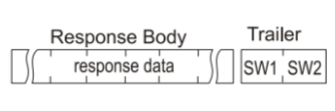
\includegraphics[width=0.55\linewidth]{gfx/APDUResponse}
	\end{center}
	\caption{APDU Response}
	\label{fig:APDUResponse}
\end{figure}




\hfil


The transmission protocol varies between different types of readers and smart cards (e.g. chip, contact-less), but what is common between every smart card interaction, is the \textit{APDU Command-Response Dialogue}. As long as the smart card has a power supply, it can maintain the dynamic memory in RAM between APDU Commands, what allows to do in two or more commmands complex operations, transmit more bytes than a single APDU can admit, etc.



\begin{figure}[bth]
	\begin{center}
		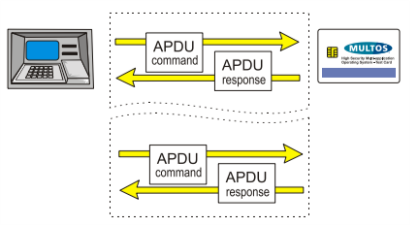
\includegraphics[width=0.75\linewidth]{gfx/APDUdialog}
	\end{center}
	\caption{APDU Command-Response Dialogue}
	\label{fig:APDUdialog}
\end{figure}



\section{P2ABCE}


In the \ac{P2ABCE} repository \citep{p2abcurl} is available the project's code, divided in two solutions: a complete P2ABCE implementation in Java and a Multos Smartcard implementation as companion for the project.

The Java code is managed by a Maven project, structured using various known design patterns, but not of our interest. The structure we are actually interested in are the REST Services and their use of the Components classes, in which the smartcards are included.

P2ABCE project is based on the concept of smartcards to store the credentials, logical or physical. An interface is defined to communicate with these smartcards, and then different implementations allow to use either \textit{Software Smartcards} or \textit{Hardware Smartcards}. 

The \textit{SoftwareSmartcard} class implements the interface in Java, suitable for tests and self-stored smartcards that any application using P2ABCE may need.

The \textit{HardwareSmartcard} class uses the standard APDU messages [TODO:ref] to interact with smartcards. P2ABCE defines for every method in the mentioned interface, the necessary APDU instructions, and currently relies on \textit{javax.smartcardio} abstract classes (implemented by Oracle in their JRE) to communicate with the smartcard reader. This way, it doesn't matter what manufacturer issues the smartcard, or if it's an Android device, if they support the APDU API, P2ABCE will work with them.

\begin{figure}[bth]
	\begin{center}
		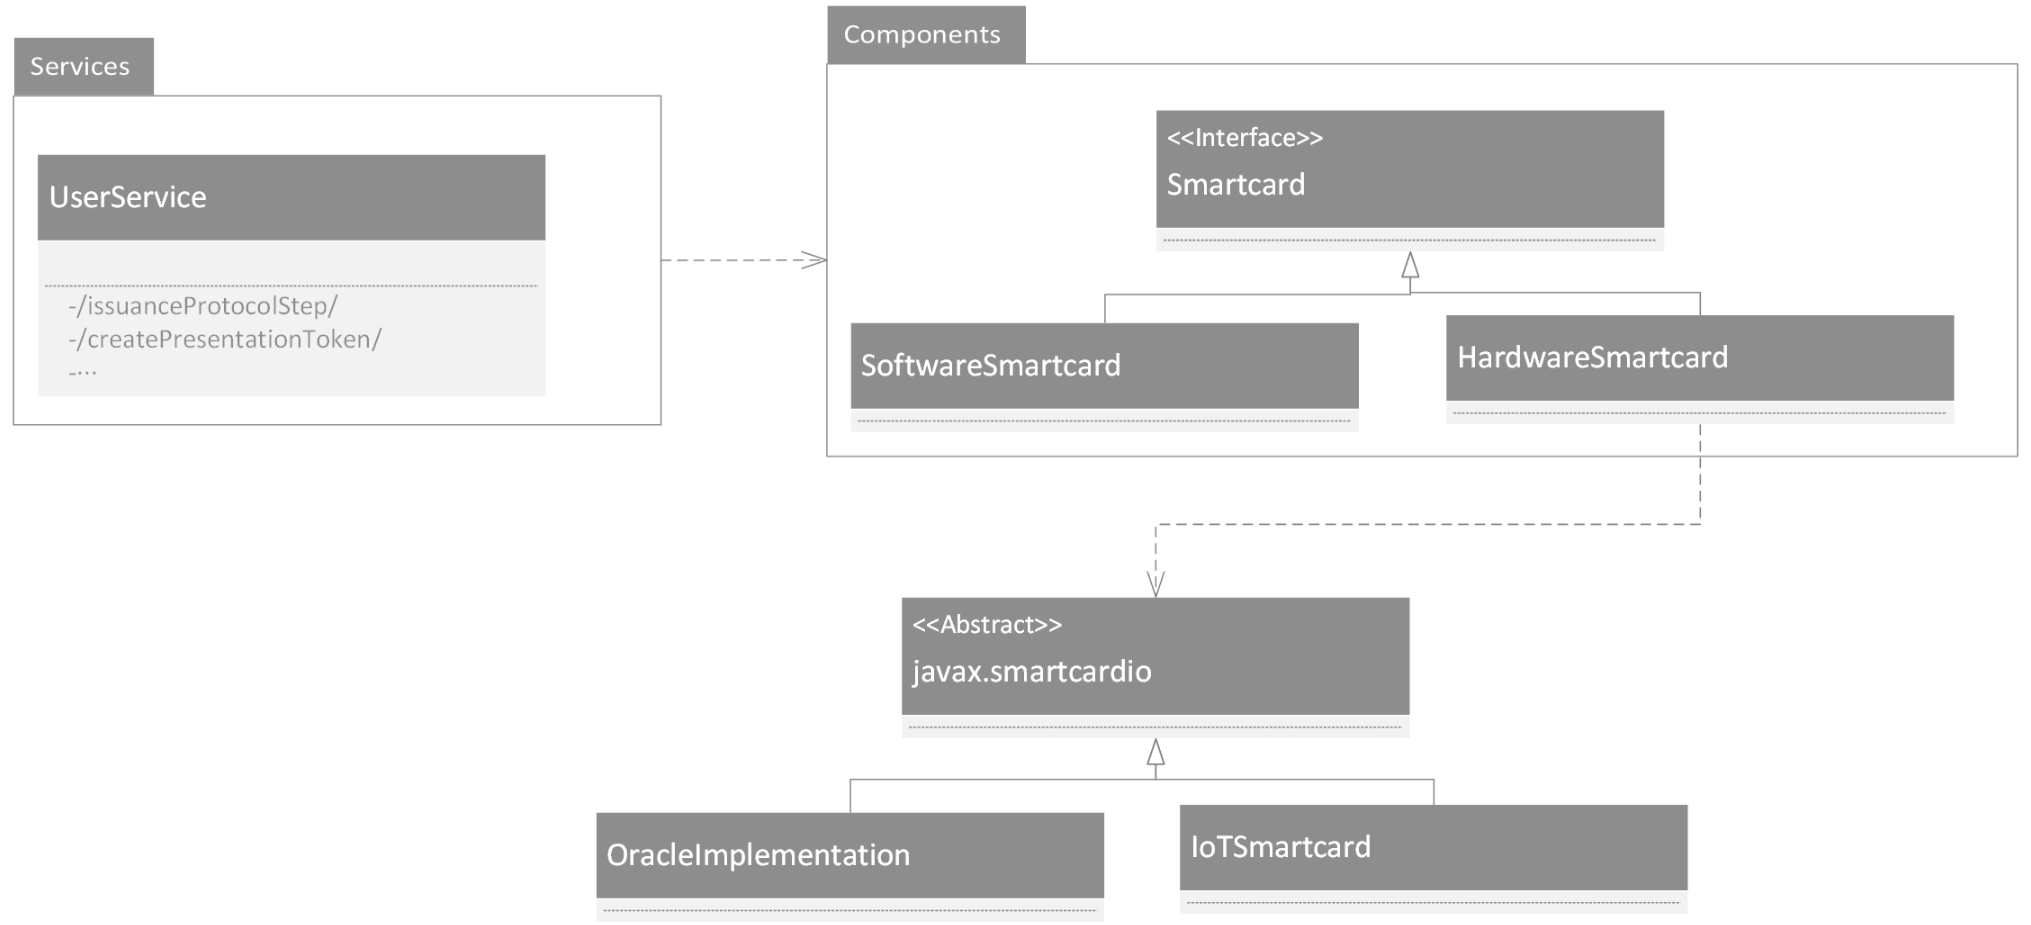
\includegraphics[width=\linewidth]{gfx/p2abceBasicUML}
	\end{center}
	\caption{Basic P2ABCE structure}
	\label{fig:p2abceBasicUML}
\end{figure}


As a PoC the P2ABCE project includes the ABC4Trust Card Lite, an implementation for ML3-36K-R1 Multos Smartcards. The code is written in C, but is very dependent on the Multos framework, aside from numerous bugs and bad coding habits. 



At this stage, we have two options to implement our IoT device compatible with P2ABCE:

\begin{itemize}
	\item Implement in C the \textit{Smartcard} interface used by P2ABCE architecture, and use some communication protocol to remotelly call the methods from the machine running the P2ABC Engine.
	\item Present the IoT device as a hardware smart card, using the APDU protocol (already defined, standard and with minimal overload). Providing a \textit{javax.smartcardio} ``IoT implementation'' to communicate with the IoT device through a transmission protocol, the already existing \textit{HardwareSmartcard} class can work with the new \textit{IoTSmartcard} in the IoT device.
\end{itemize}



%TODO : hablar más de los servicios REST



\section{MULTOS}

MULTOS is a multi-application smart card operative system, which provides a custom developing environment, with rich documentation \citep{MultosTechLib}. MULTOS smart cards communicate like any other smart card following the standard, but internally offers a very specific architecture, affecting the way one must code applications for it.

In this section we will present the main characteristics of a MULTOS smart card that shaped the ABC4Trust Card Lite code and that we had to be aware of when adapting it to IoT devices.

\paragraph{MULTOS programming languages} A native assembly language called MEL, C and, to a lesser extent, Java, are the available languages to code for MULTOS. In our case, ABC4T Card Lite uses MEL and C.

\paragraph{MULTOS Workflow}

Most of the transmission and communication process is done by MULTOS core, and it then selects, based on the CLA byte of the APDU, the application to load. This application is what most developers will only worry about, and is where their $main()$ function will start.

\begin{figure}[bth]
	\begin{center}
		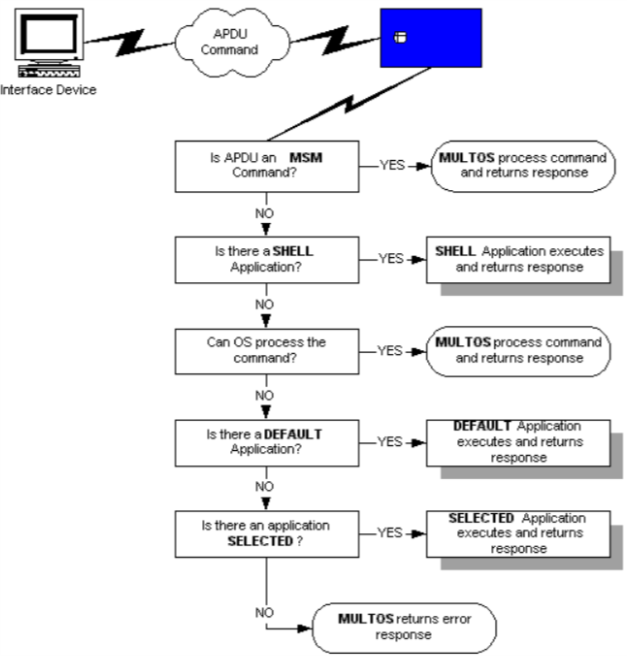
\includegraphics[width=\linewidth]{gfx/multosWorkflow}
	\end{center}
	\caption{MULTOS workflow}
	\label{fig:multosWorkflow}
\end{figure}

The application uses then the \textit{multos.h} file that declares multiple global variables already loaded with the needed data, including the APDU Command bytes.

Now the developer is in charge of checking what instruction was sent and if the APDU has the expected ISO Case. If everything is ok, code what needs to be run and write in specific data space the APDU Response bytes, call \textit{multosExit()} and MULTOS will be in charge to send the APDU Response.

In summary, our application starts with all data loaded and exits without worrying how to send the answer. A very comfortable workflow that we must now implement for our IoT device if we would want ABC4T Card Lite code to work.

\paragraph{MULTOS Memory Layout}

Each application in MULTOS has access to a specific memory layout, divided in different categories:

\begin{figure}[bth]
	\begin{center}
		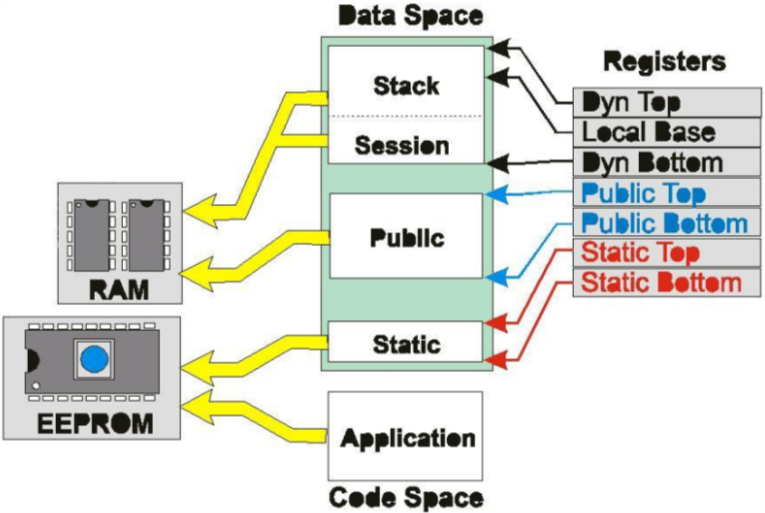
\includegraphics[width=\linewidth]{gfx/multosMemLay}
	\end{center}
	\caption{MULTOS Memory Layout}
	\label{fig:multosMemLay}
\end{figure}


The Code Space is where the application code is stored.
The Data Space is divided in Static memory, Public memory and Dynamic memory.

\textbf{Static memory} are the application variables declared after the specific \textit{\#pragma melstatic} compiler directive. These variables are stored in the non-volatile EEPROM, and any write is assured to be saved because they are not loaded into RAM.

\textbf{Public memory} can be seen as the input/output buffer for applications and MULTOS system. The APDU header appears at the top of Public, and command data at the bottom. The application writes then the APDU Response bytes in Public, at specific position (see \autoref{fig:multosPubMem}). To declare variables in this data space, the \textit{\#pragma melpublic} directive is available.

\textbf{Dynamic memory} works like usual program memory, with Session Data storing global variables and the Stack. The limited size of RAM in IoT devices and smart cards makes the use of dynamic memory not advisable. The compiler directive to use Session Data is \textit{\#pragma melsession}.


\begin{figure}[bth]
	\begin{center}
		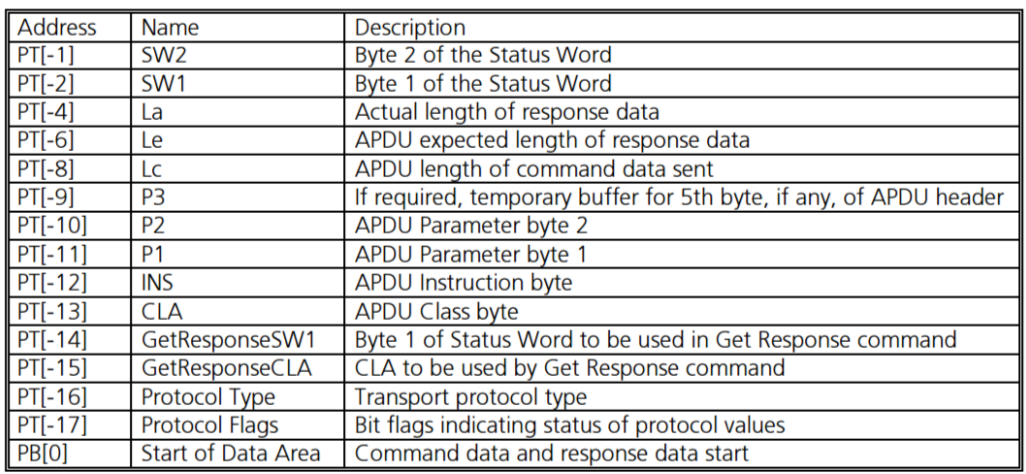
\includegraphics[width=\linewidth]{gfx/multosPubMem}
	\end{center}
	\caption{MULTOS Public Memory Data Map}
	\label{fig:multosPubMem}
\end{figure}


\hfil


With regards to primitive types, to avoid confusion with their sizes, MULTOS defines and uses the following data types specified in \autoref{fig:multosDataTypes}. It's important to notice that MULTOS is Big Endian
\marginpar{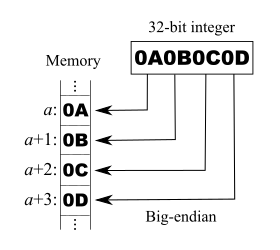
\includegraphics[width=\linewidth]{gfx/Big-Endian}\\Big-Endian, Wikipedia}
and when storing structures there is no padding between defined variables, unlike modern compilers that perform data structure alignment \citep{dataStructAlign} for performance.

\begin{figure}[bth]
	\begin{center}
		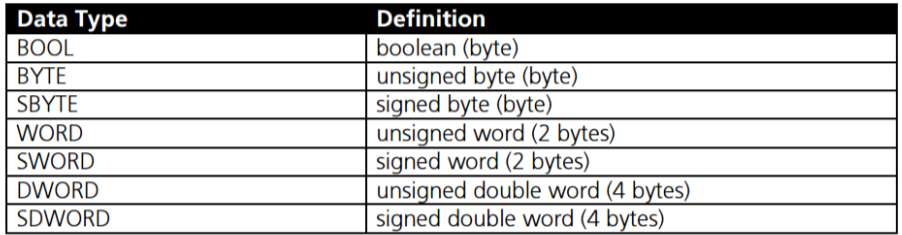
\includegraphics[width=\linewidth]{gfx/multosDataTypes}
	\end{center}
	\caption{MULTOS Data Types}
	\label{fig:multosDataTypes}
\end{figure}


\paragraph{MULTOS Standard C-API}

A collection of more than a hundred functions are provided for arithmetic, cryptography, memory and smart card operations. The \textit{multos.h} interface provides access to these functions, that ultimately call their respective primitive instructions in assembly code. The primitive instructions are but a system call with an operation code, loading data in the needed registers. Therefore,  no implementation for these tools is available, nor in C, nor in assembly code.

Nevertheless, the C-API documentation \citep{MultosTechLib} provides rich description for each function.





\section{ABC4Trust Card Lite}

P2ABCE provides a smart card reference implementation, ABC4Trust Card Lite \citep{ABC4TCardLite}. It supports device-bound U-Prove and Idemix, and virtually any discrete logarithm based pABC system.

Version 1.2 is based on MULTOS ML3 cards, with approximately 64KB of EEPROM (non-volatile memory), 1KB of RAM and an Infineon SLE 78 microcontroller, a 16-bit based CPU aimed for chip cards.

The card stores the user's private key $x$ and any \ac{BLOB} that the P2ABCE may need (like user's credentials). Then P2ABCE delegates the cryptographic operations on the smart card, that operates with $x$.

\begin{figure}[bth]
	\begin{center}
		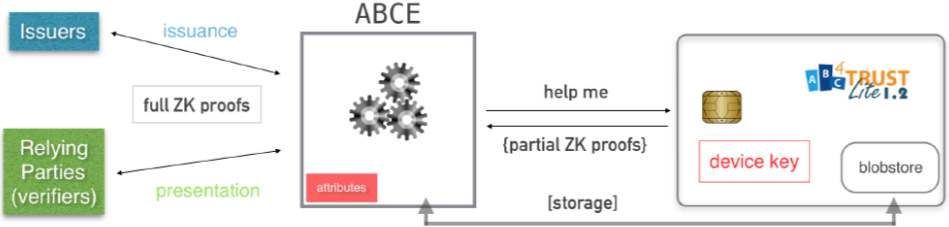
\includegraphics[width=\linewidth]{gfx/ABC4TCardLite}
	\end{center}
	\caption{ABC4Trust Card Lite}
	\label{fig:ABC4TCardLite}
\end{figure}

The cryptographic operations performed by the smartcard are the modular exponentiation and addition that discrete logarithm ZKPs are based on.

\hfil

The code is available from the P2ABCE project and has some good and bad points to have in count:

The best asset of this code is that it's written in C aiming to a very constrained device, similar in computational power to many IoT devices, and very limited memory.
	
Some \textit{tricks} in the code include using \textit{union} data types for variables that will be stored on the same data location, but at different moments (e.g. depending on APDU Command INS byte), minimizing this way the use of RAM and making code readability better; or strong use of pointers and \textit{memcpy} calls to copy structures with multiple variables as arrays of bytes.


Among the many drawbacks, we could highlight the awful coding, the strong dependency on MULTOS framework and some bugs found. 

The code is structured in two files, \textit{main.h} and \textit{main.c}, with 557 and 5157 lines of code respectively.

The file \textit{main.h} is mostly a reimplementation in assembly MEL of some MULTOS functionality already offered with latest \textit{multos.h}.

The \textit{main.c} consists on near 600 lines of variables and data structures declarations, followed by the \textit{main()} function, a 2635 lines long \textit{switch-case} with practically no comments, and to conclude, the implementation of thirty functions called \textit{Subroutines} at the end of the file.


This gives an idea of the problematic to maintain or even understand the code. But once one studies MULTOS framework in deep and applies many refactoring techniques to ABC4T Card's code, this becomes the best starting point for the IoT version.





\section{IoT and P2ABCE}

In this section we will define how an IoT device will be integrated in the P2ABCE environment, being totally compatible with any other system using P2ABCE, addressing the power and memory constrains IoT devices face.


\hfil

Our main goal is to make an IoT device capable to act as an User or Verifier in the P2ABCE architecture. For this, the device should manage complex XML schemas, perform cryptographic ZKP operations and communicate with the Verifier or Prover with which it's interacting.

The communication is already solved by the \textit{Internet} capabilities of IoT devices.

Our concern are the data artifacts exchanged as XML and the cryptographic operations involving secret keys that must remain private to the IoT device.

Here is where we look at the P2ABCE architecture more closely, and the concept of smart cards shows a solution for the second issue. Even in the case we were to implement all P2ABCE inside an IoT device, we would have to implement support for software smart cards, to keep the secret inside the IoT device. We will start building the house from the ground, implementing the smart card operations inside the IoT device.

Now that in our design we have the smart card, we need to address the first point, XML squemas. We understand with \textit{XML squemas} both managing the XML syntax and the whole process to generate a proper answer, that is, basically, the crypto engine that relies on Idemix and the smart card to hold the secret information.

Taking in consideration Idemix is currently provided in Java as a considerably big project, and version 3.0.36 still hasn't got official documentation, the task to port the Idemix crypto engine to IoT could be done in the future, if the chosen devices have enough storage and capacity. And even in that case, we would need to implement P2ABCE User and Verifier's architecture to completely free ourselves from an external P2ABCE machine.

The final port would be so big, many IoT devices would fall out of the requisites to run it, failing in our initial objective.

\hfil

After this analysis of the P2ABCE, we conclude that the mandatory requisite for any IoT device that wants to work with this system and keep its private keys in it, is to implement the smart card functionality, and delegate the rest of the operations on a machine capable of running P2ABCE, until that functionality is implemented for the IoT device. 


\hfil

This architecture is not really such an original idea. For example, IPv6 involves managing 128 bits per address and large headers, and many use cases only need IoT devices to communicate inside a private network. That's why many of them use 6LoWPAN to compress packets or use smaller address sizes. To communicate a 6LoWPAN with the Internet, a proxy is needed to transform 6LoWPAN packets to IPv6.

\hfil


Therefore, the IoT device now has a \textbf{duality} in its functions, because it is the User that starts any interaction with other systems, and it's also the smart card that P2ABCE delegates for crypto operations. It can also be seen as a \textbf{double delegation}. The IoT device delegates on the external P2ABCE server to manage the protocol, and the P2ABCE server delegates on the IoT, acting now as a smart card, for the cryptography.




\hfil

We find here two challenges: how to delegate from the IoT device to the P2ABCE delegation server, and how to transmit them and the APDUs to the IoT device.

Currently P2ABCE offers various REST web services to run different roles in P2ABCE system: User Service, Issuer Service, Verification Service, etc. An application that integrates P2ABCE can make use of this services in the same machine or implement the functionality using the core components written in Java, the same ones the REST services use. Our PoC machine, the Omega2, can make REST calls easily, but other devices may use \ac{CoAP}, and in that case, the P2ABCE REST services should be rewritten to offer CoAP support. The commands needed to delegate to the P2ABCE delegation server will be the same to operate with the REST services. This way, the first issue is solved.

The transmission of the messages will depend on the specific use case, capabilities and resources available. If the delegation server is connected, for example, through RS-232 serial with the IoT device, and physically inaccessible, in the same way an IoT device on its own would be protected, the communication is simple, and not far away from the Arduino Yun idea of combining two devices, one more powerful but to use only when needed. But if the IoT device and the delegation server are apart, or more than one IoT device delegates to it, then the transmission must be secured. They could use 6LoWPAN to talk to each other (the delegation service could be deployed in the proxy) and then secure communications with existing solutions, like with pre-shared symmetric keys, certificates for authentication and authorization, etc., it depends on each particular deployment.

At the end of the day, this is all about usual security in IoT. Many other studies focus on this matter, so we will assume it can be done, and will focus on what's new, P2ABCE in IoT.


\hfil


% TODO: imagen con servicios desplegados/actores en cada máquina


To sum up, our IoT device will act as User (Prover or Verifier) keeping its secrets in a software smart card. When it starts an interaction with other actor of the P2ABCE system (Issuer, Verifier, etc.), the IoT device will delegate with a remote call (using REST in our PoC) to a P2ABCE delegation server, attaching the XML file and the necessary information for the server to send the APDUs to the software smart card (in our PoC using TCP sockets, giving the IP and listening port).



\begin{figure}[bth]
	\begin{center}
		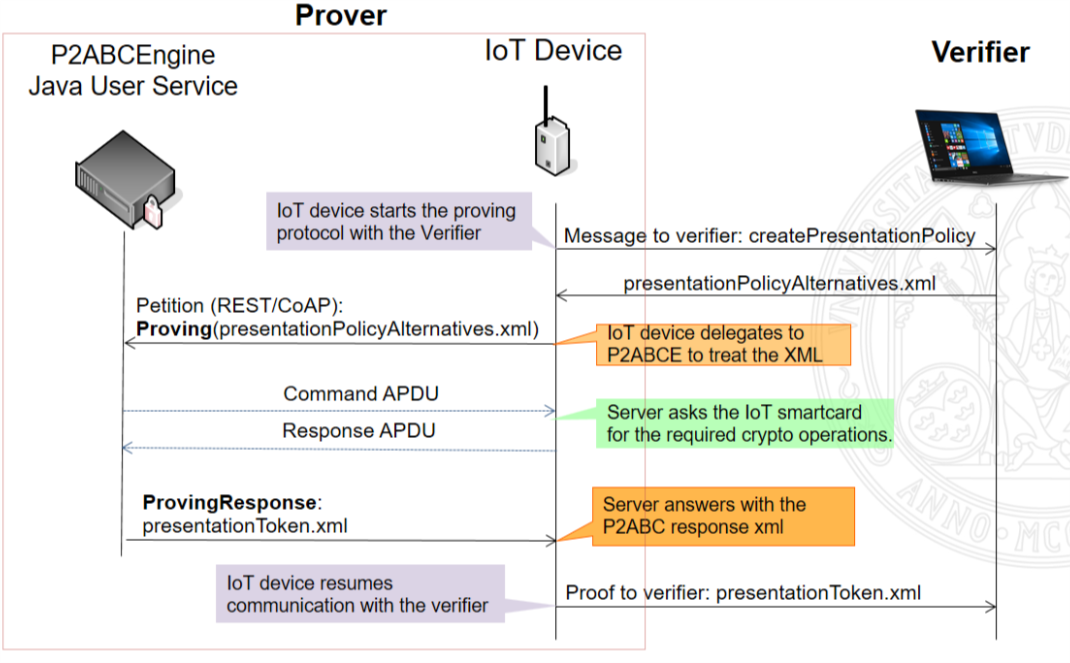
\includegraphics[width=\linewidth]{gfx/DelegationProving}
	\end{center}
	\caption{IoT Delegation in P2ABCE for Proving.}
	\label{fig:DelegationProving}
\end{figure}


\hfil


This simple design keeps the benefit of a 100\% compatible P2ABCE deployment, and the integration of IoT devices to the P2ABCE ecosystem.

In the future, more functionality currently delegated in the P2ABCE server can be implemented in the IoT device, if its resources allow it. For example, in a M2M environment, where an IoT device can act as User and Verifier, the verification consists on sending a Presentation Policy, and verifying the Presentation Token, which implies less logic than generating it as the User. Therefore, the implementation of the Verifier functionality would reduce significantly the need of a delegation server, but as we said, managing complex XML squemas is not something many IoT devices could do.




\section{IoT Smart Card}

After many design decisions in the process to adapt the original ABC4T Card Lite code to pure C, working over a more usual architecture machine, in this section, we present the current \ac{PoC} code, most important decisions, workflow execution, and future work.

First, let's define what a \textit{more usual architecture} is. If we remember the MULTOS section, the framework gives an application a very specific memory layout and entry and output points of execution, that could be seen as a single process execution machine. Many IoT devices work like a computer, with multiple processes or threads, without pre-loaded data on startup (like the APDU MULTOS loads for the application), a non-volatile memory for data and code, maybe a basic file system in this memory, and RAM with the program's stack, heap, data and code.

Our PoC is tested on a Linux system, and we will give instructions on how to adapt each part to work with other typical IoT systems.
For example, other IoT devices may work like MULTOS and let access variables in non-volatile memory during execution, and in that case, the port should be changed according to these particularities.


\hfil

\begin{figure}[bth]
	\begin{center}
		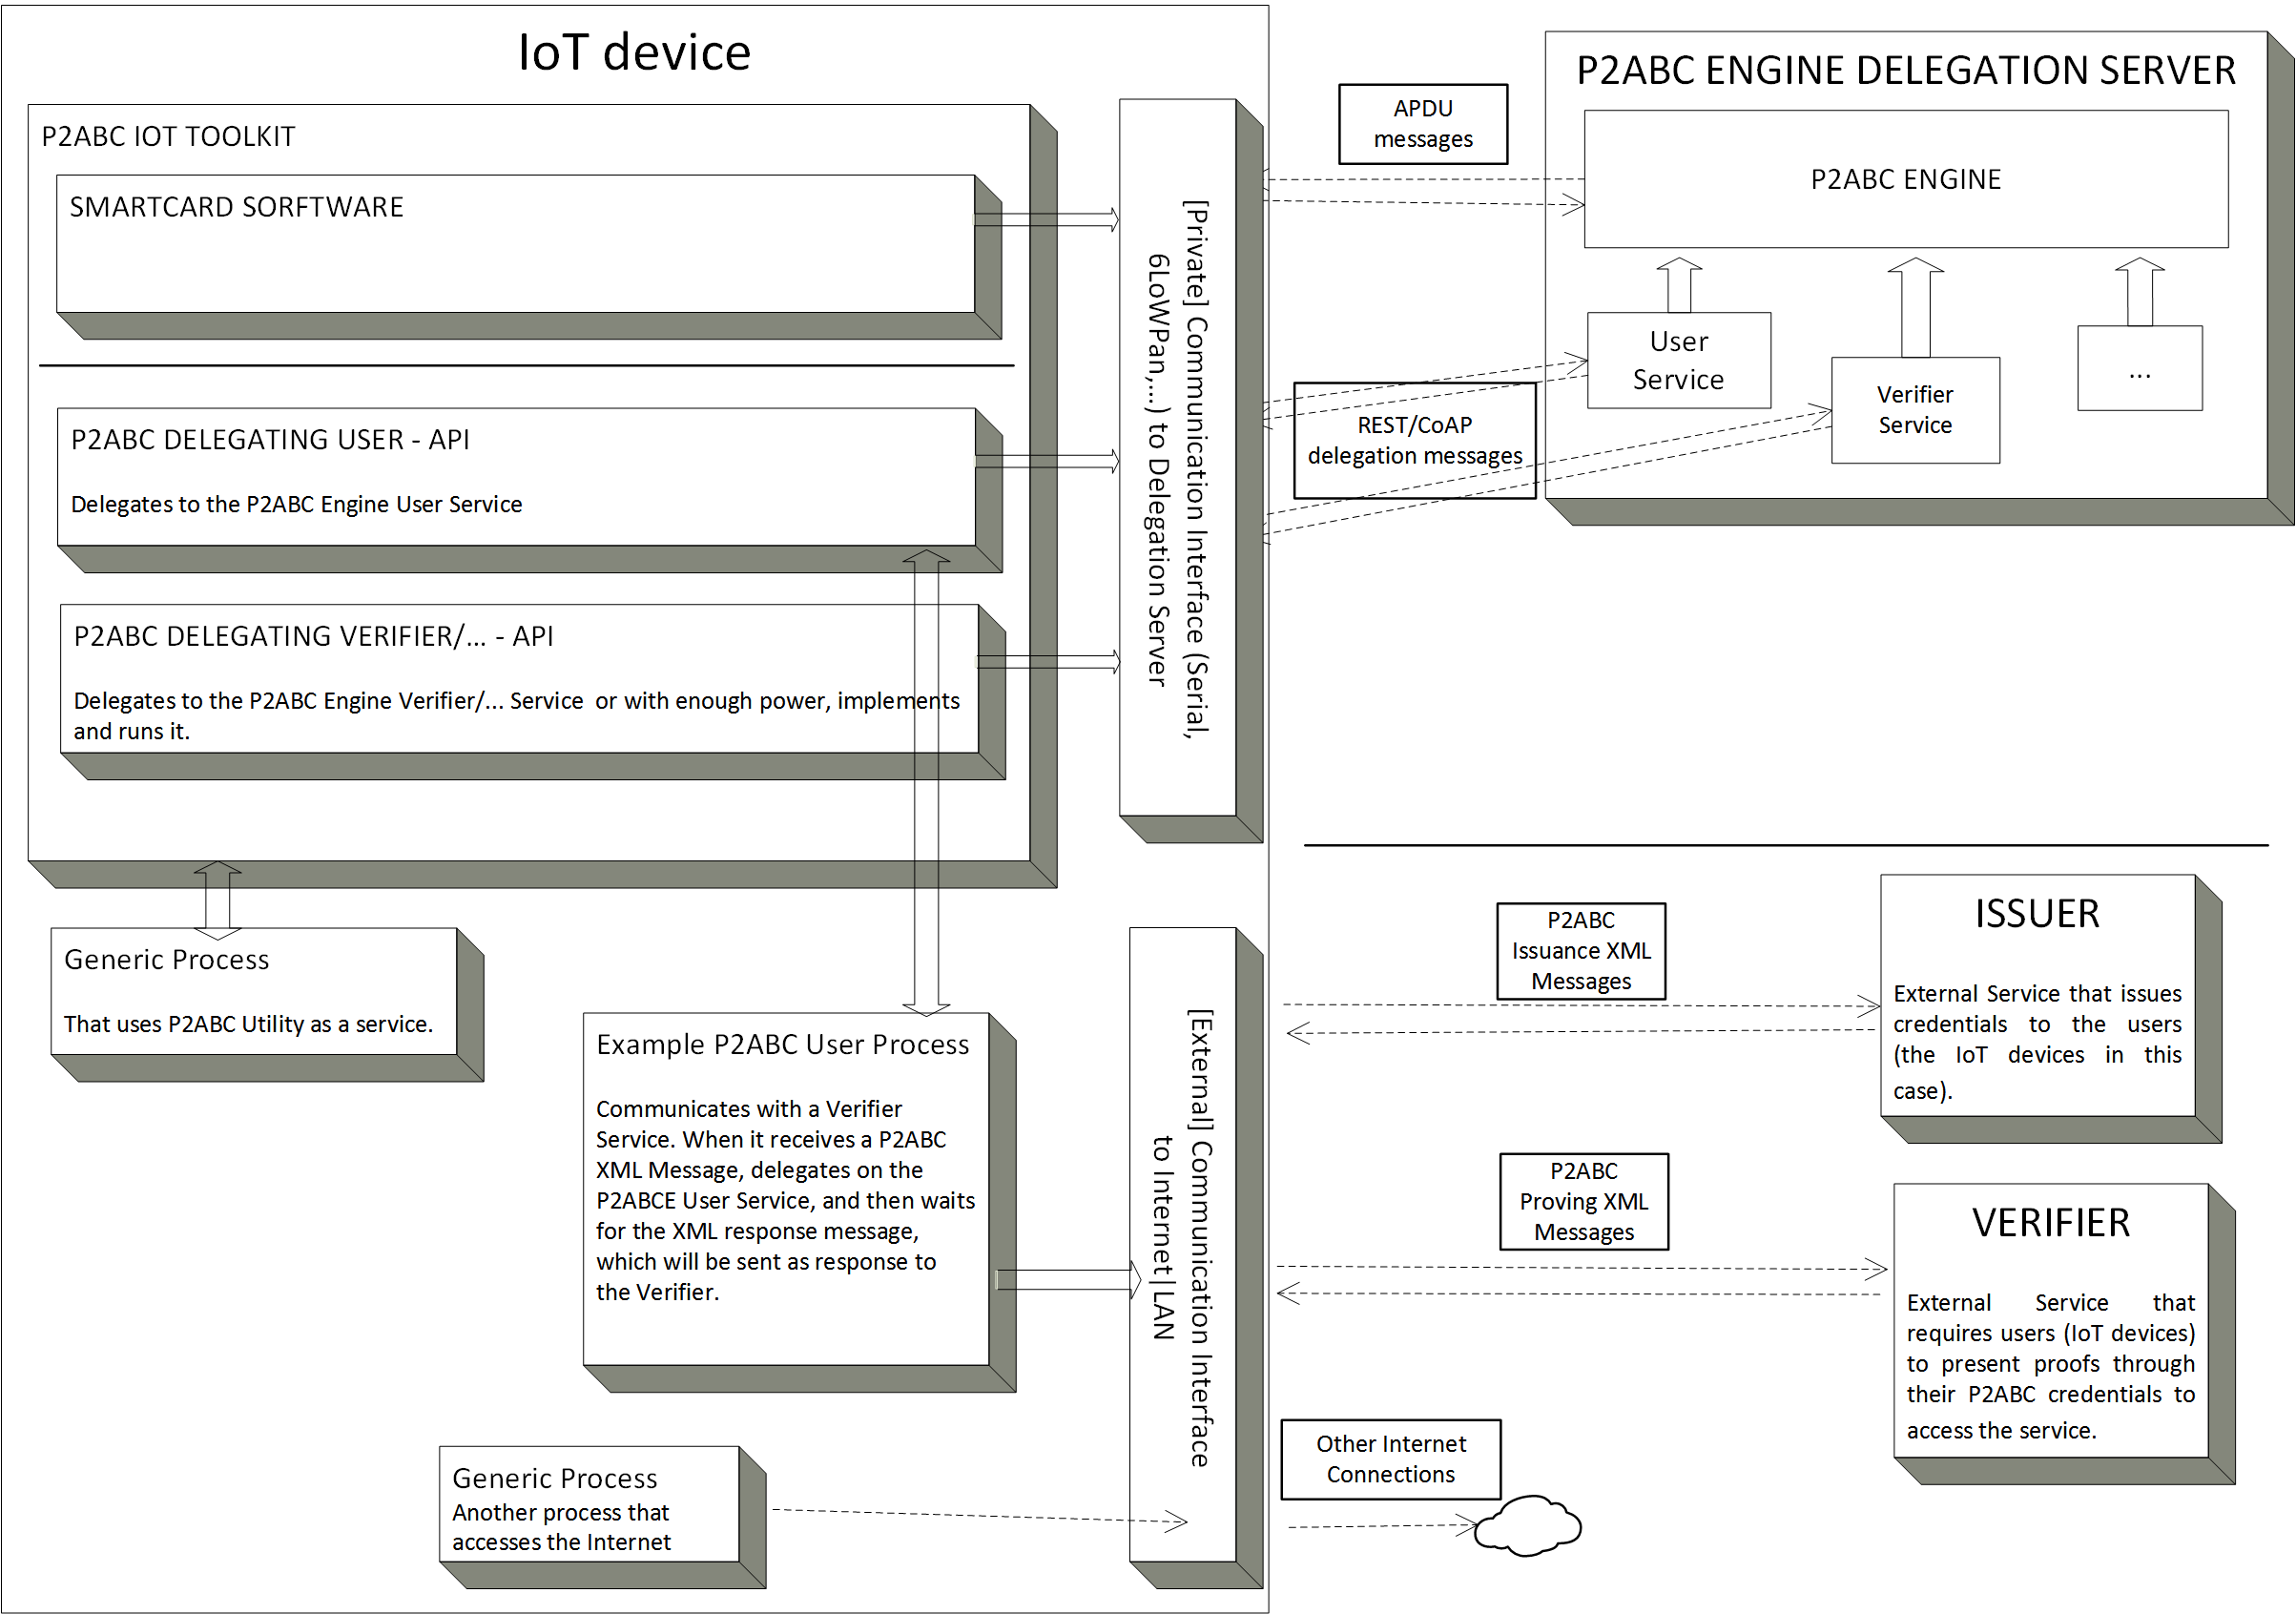
\includegraphics[width=\linewidth]{gfx/P2ABCE-IoT-bw}
	\end{center}
	\caption{P2ABCE-IoT.}
	\label{fig:P2ABCE-IoT}
\end{figure}

\begin{figure}[bth]
	\begin{center}
		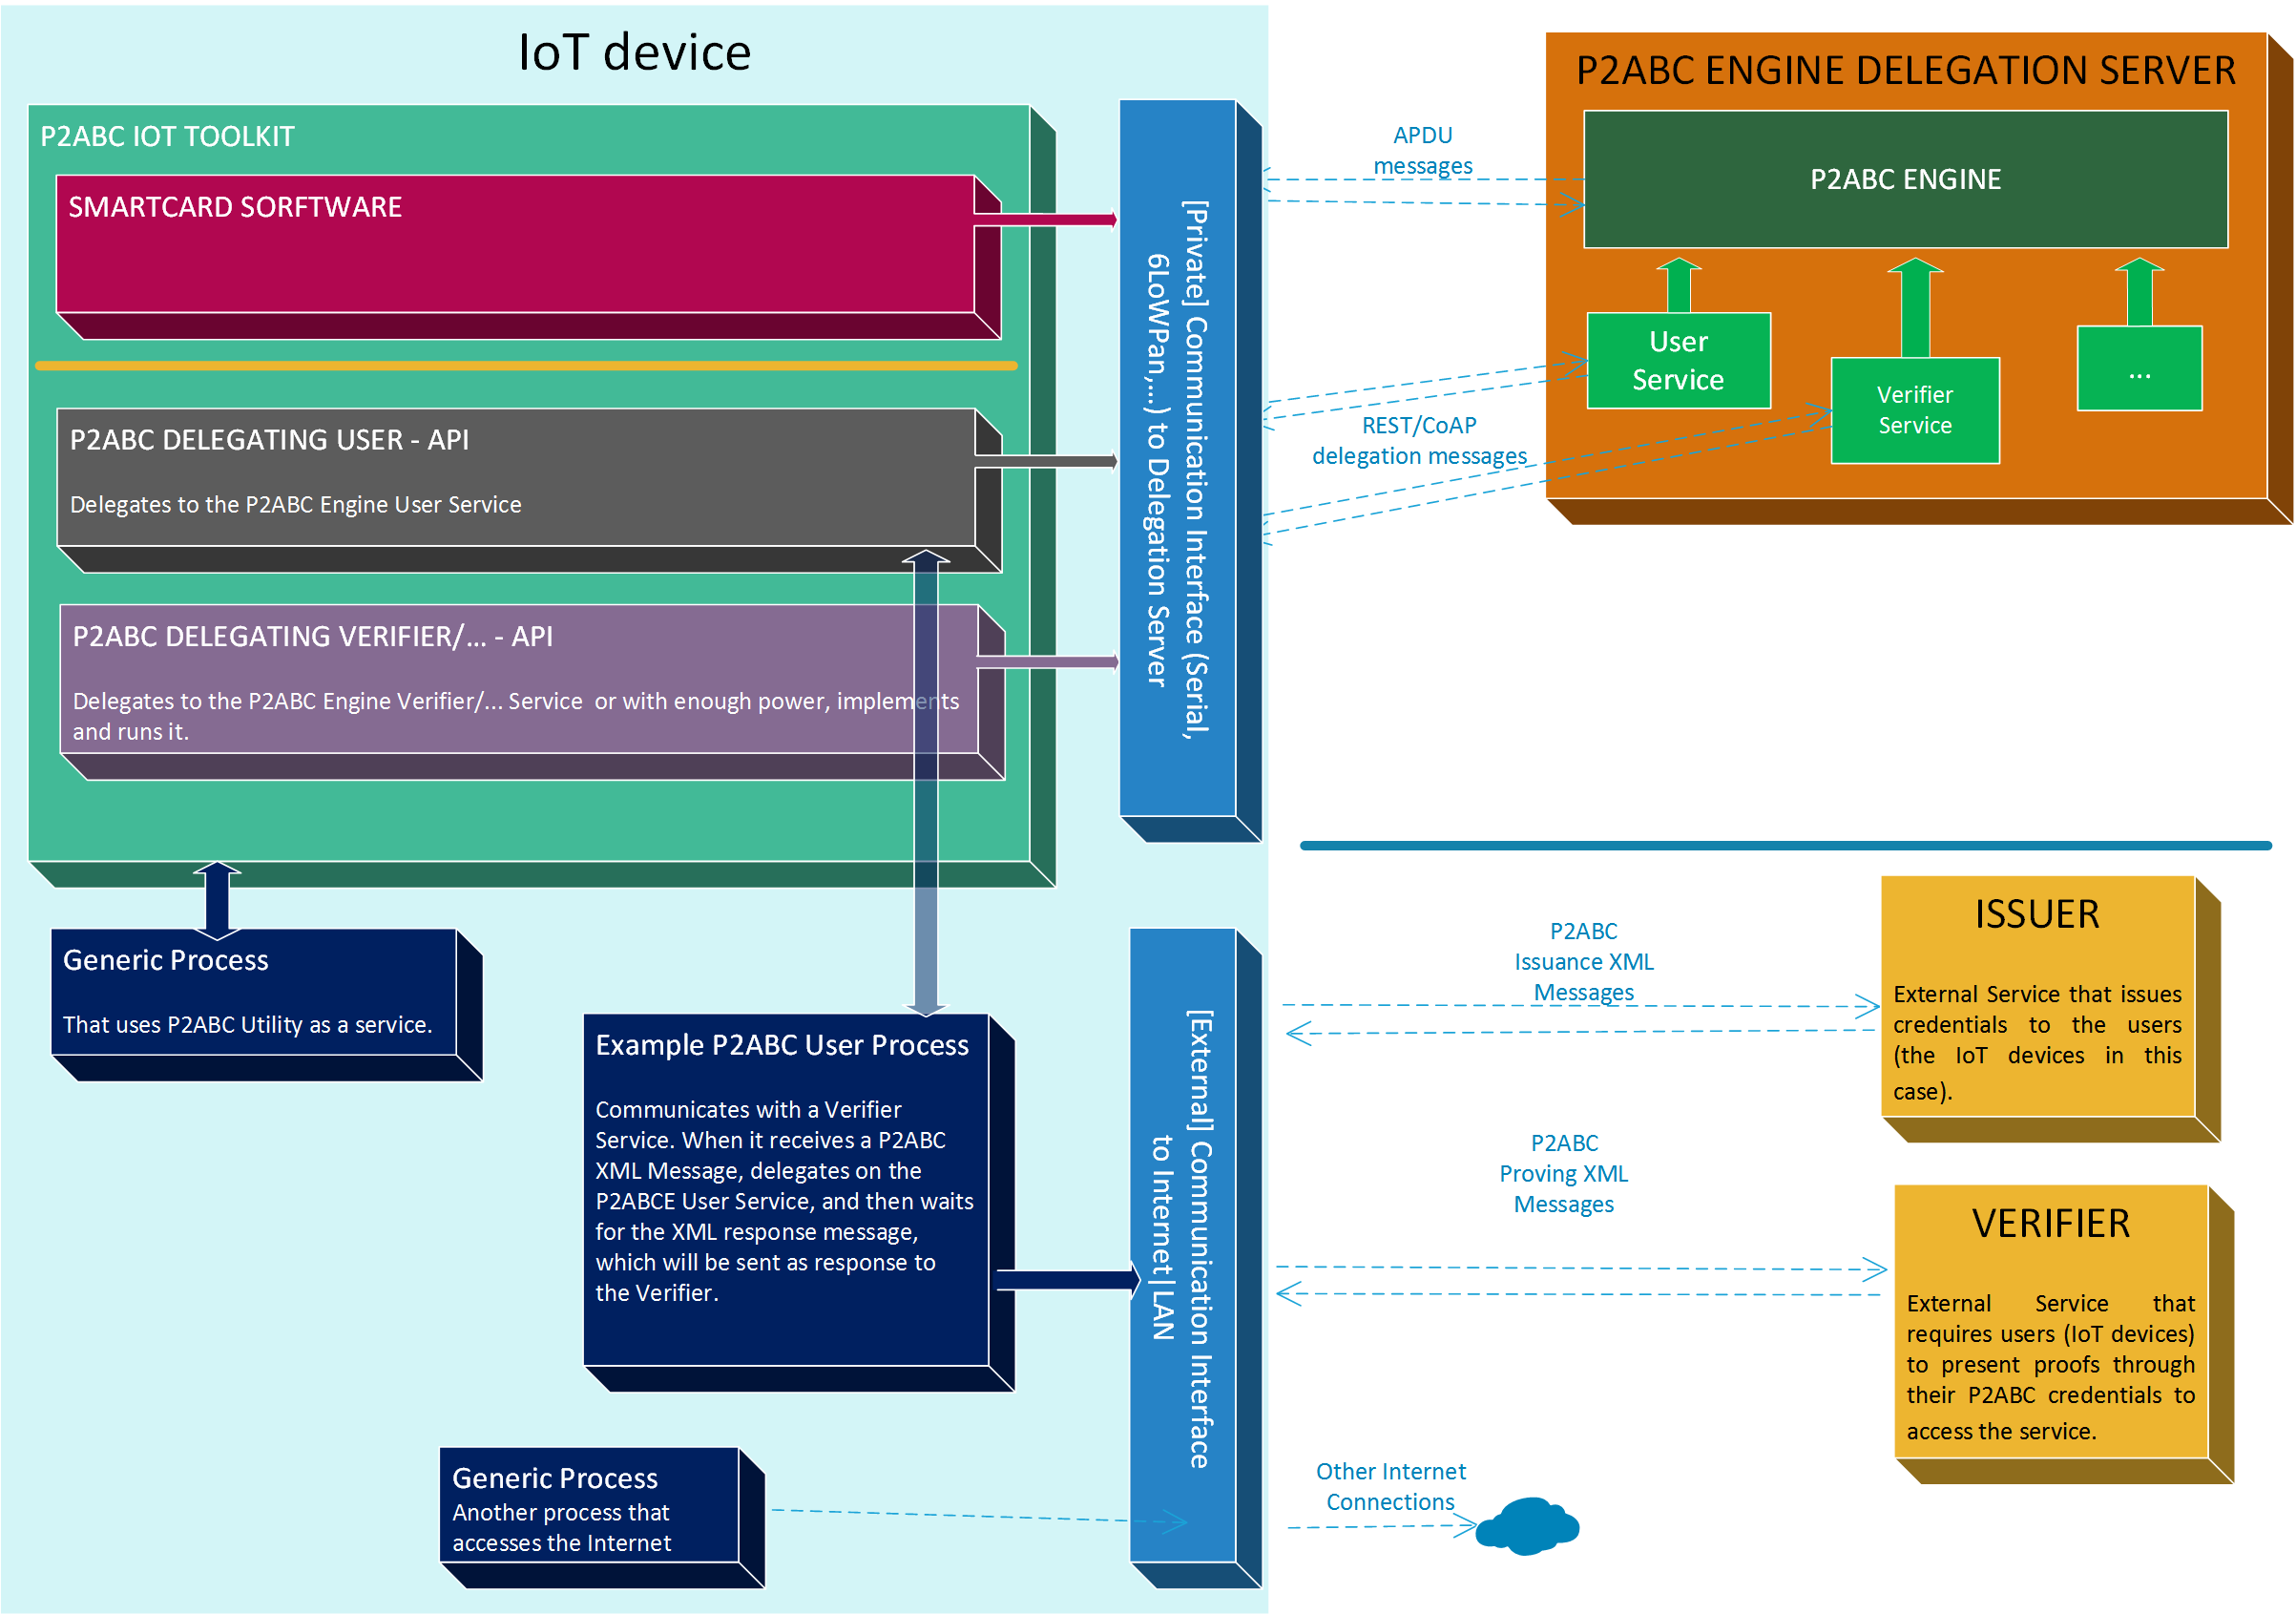
\includegraphics[width=\linewidth]{gfx/P2ABCE-IoT-color}
	\end{center}
	\caption{P2ABCE-IoT-color.}
	\label{fig:P2ABCE-IoT-color}
\end{figure}



\subsection{Code structure}


We divide the project in three different sections with the objective of enhancing maintainability, improving future changes, ports, fixes, etc.

The first section is what could be called as the core of the smart card, the second one the interface for the tools the core need and may depend on the platform, and finally third party libraries, that in may be empty if the interfaces implementation doesn't need any.


In our PoC we used CMake to manage the project, due to the cross-compilation tools, integration with multiple IDEs and tests.


\begin{figure}[bth]
	\begin{center}
		\includegraphics[width=\linewidth]{gfx/IoTCScomponents-color}
	\end{center}
	\caption{IoT Smart Card Code Structure.}
	\label{fig:IoTCScomponents-color}
\end{figure}

\begin{figure}[bth]
	\begin{center}
		\includegraphics[width=\linewidth]{gfx/IoTCScomponents-bw}
	\end{center}
	\caption{IoT Smart Card Code Structure.}
	\label{fig:IoTCScomponents-bw}
\end{figure}


\hfil

\paragraph{Core smart card}

The smart card logic lies in this section, the concepts of APDU Commands, what instructions are defined in P2ABCE smart cards and how to process them and generate proper APDU Responses.

Changes in the APDU protocol for P2ABCE must be done here, independently of the target platform.

After refactoring the original ABC4Trust Card's code, most of it fell in what we will call the core of the smart card.

All types and variable definitions and the APDU handling is done in this code.
However, the ABC4Trust's code depended on the MULTOS C-API for the input/output of data, modular arithmetic, and even AES128 and SHA256 cryptography.

A characteristic of MULTOS C-API is that every function name starts with \textit{multos}, but as we said, the \textit{main.h} file implemented equivalent functions to some available in \textit{multos.h}. Our first step was to replace the \textit{main.h} functions for the standard ones in the C-API. Then, we implemented, following the C-API documentation, the functions from \textit{multos.h} (only the used ones) changing their names from \textit{multosFoo()} to \textit{mFoo()} for readability and emphasize that they were no longer from MULTOS.

Future changes in the code may refactor it so there's no longer need for the MULTOS framework functions.


\paragraph{Interfaces}

To implement MULTOS functions, we needed to use some libraries, so we defined a facade to isolate the implementation of the core smart card from our different options, that could vary depending on the hardware or the system used by the IoT device.

The use of a facade lets us, for example, change the implementation of modular arithmetic with a hardware optimized version, or a future more lightweight library, or our very own software implementation using the same data types that the core uses, minimizing the data transformations needed.

Taking a step forward, we make the core smart card totally independent of any library, only on our interfaces. This means that typical C libraries, like the standard \textit{stdlib.h}, or  \textit{string.h} are also behind the facade, in case some IoT system doesn't support them. The main goal we go after with this decision is that future developers adapting the code to a specific platform need to make no change to the \textit{core smart card}'s code, only to the interfaces implementation.



\paragraph{External utilities}

If the IoT system offers well tested libraries that could aid in the interfaces implementation, or we simply found a pure C implementation for the task, these third party libraries belong to this section.

In our PoC, we use two ANSI C libraries, for base64 and JSON, and two shared libraries available in as packages in LEDE, GMPLib and OpenSSL. The last two libraries offer more functionality than we need, hence, it's desired in a production code to implement \textit{Modular Arithmetic} and \textit{Cryptography} interfaces with more lightweight alternatives.

For example, Atmel's ATAES132A \citep{ATAES132A}
\marginpar{\includegraphics[width=\linewidth]{gfx/atmel} \\ Atmel's cryptography chips.}
offers a serial chip for secure key storage, AES128 execution and random number generation. Another serial chip like ESP8266 offers WiFi connectivity, typically used with Arduino, and can also perform AES encryption. For random number generation, a technique used with Contiki devices is to read from sensors aleatory data and use it as seed. All these alternatives depend on the target device, but are all valid. The \textit{interfaces} and \textit{external utilities} sections allow for a clean and fast port of the code.


\subsection{PoC Workflow}

% PoC BIOSC : TCP sockets, JSON serialization

% PoC IoT javax.smartcardio : protocolo de 2 bytes + APDU

% 1. Boot: deserialize sc status
% 2. Listening: open tcp socket
% 3. The IoT device delegates on the P2ABCE for some task and sends the IP and Port of the IoT Smart Card.
% 4. An APDU Command arrives : read in 2 bytes the length of the apdu and 


% ********************************************************************
% Backmatter
%*******************************************************
\appendix
%\renewcommand{\thechapter}{\alph{chapter}}
\cleardoublepage
\part*{Appendix}
%********************************************************************
% Appendix
%*******************************************************
% If problems with the headers: get headings in appendix etc. right
%\markboth{\spacedlowsmallcaps{Appendix}}{\spacedlowsmallcaps{Appendix}}



\chapter{Test: APDU Commands exchanged}\label{ch:resultsdiagrams}


In this appendix we provide 3 sequence diagrams highlighting the APDU Commands exchanged during our testbed. 


The first one is the setup of the IoT smart card, storing the system parameters needed to work in the deployed P2ABCE system. The first Command is called \texttt{isAndroid} because the \texttt{HardwareSmartcard} class distinguishes Android phones acting as smart cards from MULTOS smart cards, in order to use Extended APDUs. Then configures the smart card, setting the PIN (``\texttt{1234}'' by default) and PUK. Finally, it copies the cryptographic system parameters to the smart card with multiple \texttt{SET} instructions.

The second image shows the issuance of the credential, divided in the three REST calls needed during the delegation. If we recall Idemix's issuance protocol, the User performed, during his first step, an exponentiation with his secret key and a ZKP, which can be identified by the \texttt{COMMITMENT} and \texttt{ISSUANCE RESPONSE} commands. During the second step, the User only has to verify the Issuer's ZKP and store the credential if the signature is valid. Because the P2ABC Engine can perform Verification of ZKP without the need of secret keys stored in the smart card, the APDU Commands in this phase are only for storing the credential information inside the IoT smart card's BLOB\footnote{\textbf{B}inary \textbf{L}arge \textbf{Ob}jects} database, with the \texttt{STORE BLOB} instruction. 


The last diagram represents the proving for the Presentation Policy received from a Verifier, using two REST calls. During the first REST call, the Service stores data for the proving in the smart card, but before starting the proving itself, the device must choose an identity for the proving. This is done with the Identity Service, that in the PoC chooses the first identity available. After this, the second REST call starts the proving, creating the \textit{commitment} and \textit{responses} that integrate any ZKP, and depends on the device's secret keys\footnote{We, again, refer the reader who wants to know more about ZKPs to \citep{tfgmates}.}.


\begin{figure}[bth]
	\begin{center}
		\includegraphics[width=0.9\linewidth]{gfx/UML/APDUsInitIoTSC}
	\end{center}
	\caption{Init IoT Smart Card APDU Commands exchanged.}
	\label{fig:APDUsInitIoTSC}
\end{figure}

\begin{figure}[bth]
	\begin{center}
		\includegraphics[width=0.78\linewidth]{gfx/UML/IssuanceAPDUs}
	\end{center}
	\caption{Issuance APDU Commands.}
	\label{fig:IssuanceAPDUs}
\end{figure}

\begin{figure}[bth]
	\begin{center}
		\includegraphics[width=\linewidth]{gfx/UML/APDUsProving}
	\end{center}
	\caption{Proving APDU Commands.}
	\label{fig:APDUsProving}
\end{figure}



\chapter{Paper proposal for JCR Magazine}\label{ch:JCR}

\includepdf[pages=-]{Chapters/bare_jrnl.pdf}


\chapter{Project's code structure}\label{ch:code}

Given the size of the project, we identify four main directory structures to arrange the code.


First, the Dockerfiles, scripts that automatize the creation of Docker images. These images are like virtual machine snapshots, although Docker is not a virtualization system, and we use the images to create containers, that are like new virtual machines started from the snapshots. We use two Dockerfiles, one for the P2ABCE compilation environment, with Java and Maven, and another one for building the Omega2 binaries, using the LEDE SDK.


\dirtree{%
	.1 Docker/. 
	.2 P2ABCE/. 
	.3 Dockerfile. 
	.3 idemix-3.0.36-binaries/. 
	.2 LEDE SDK/. 
	.3 Dockerfile. 
}

\hfil

The original P2ABCE project is of considerable size, but we list here the most interesting directories that we had to modify to make the project compatible with IoT smart cards.

\hfil

\dirtree{%
	.1 P2ABCE/. 
	.2 Code/. 
	.3 core-abce/. 
	.4 abce-components/. 
	.5 src/main/java/eu/abc4trust/smartcard/. 
	.6 IoTsmartcardio/.
	.7 util/. 
	.8 IoTsmartcardConnection.java.  
	.7 IoTCard.java. 
	.7 IoTCardChannel.java. 
	.7 IoTCardTerminal.java. 
	.6 HardwareSmartcard.java. 
	.6 SoftwareSmartcard.java. 
	.4 abce-services/. 
	.5 src/main/java/eu/abc4trust/services/. 
	.6 UserService.java. 
	.6 VerificationService.java. 
	.6 IssuanceService.java. 
}



\hfil

The IoT smart card toolkit is the core of this project. Managed with CMake, we see the \texttt{CMakeLists.txt} files, including the \texttt{Toolchain-omega2-mipsel.cmake} file with the cross-compiler information. We divide the project between the \textit{source} C files, and the header C files. Inside these directories, the organization is as stated in the implementation chapter: \textit{core} or \textit{common}, \textit{util interfaces} and \textit{external utilities}.

\hfil

\dirtree{%
	.1 p2abce\_iot\_toolkit/. 
	.2 CMakeLists.txt. 
	.2 Toolchain-omega2-mipsel.cmake. 
	.2 util\_sc\_tests/. 
	.2 util\_sc/. 
	.3 CMakeLists.txt. 
	.3 BIOSC.c. 
	.3 p2abc\_iot\_toolkit\_src/. 
	.4 smartcard\_common/. 
	.5 APDU\_handler.c. 
	.5 global\_vars.c. 
	.5 m\_adapted\_API.c. 
	.5 subroutines.c. 
	.4 smartcard\_external\_utilities/. 
	.5 cJSON.c. 
	.4 smartcard\_utils\_interface/. 
	.5 APDU\_IO\_util.c. 
	.5 arithmetic\_util.c. 
	.5 crypto\_util.c. 
	.5 serialize\_util.c. 
	.5 system\_funcs.c. 
	.3 p2abc\_iot\_toolkit\_include/. 
	.4 error\_codes.h. 
	.4 macrologger.h. 
	.4 smartcard\_common/. 
	.5 APDU\_handler.h. 
	.5 APDU\_types.h. 
	.5 abc4T\_types.h. 
	.5 defs\_consts.h. 
	.5 defs\_errs.h. 
	.5 defs\_ins.h. 
	.5 defs\_types.h. 
	.5 global\_vars.h. 
	.5 m\_adapted\_API.h. 
	.5 subroutines.h. 
	.4 smartcard\_external\_utilities/. 
	.5 base64.h. 
	.5 cJSON.h. 
	.4 smartcard\_utils\_interface/. 
	.5 APDU\_IO\_util.h. 
	.5 arithmetic\_util.h. 
	.5 crypto\_util.h. 
	.5 serialize\_util.h. 
	.5 system\_funcs.h. 
}


\hfil

Finally, the test scripts, including a Python file to test the BIOSC protocol, a directory with the testbed scripts (one file to orchestrate every device from one terminal), and a more didactic version with a script per device.

\hfil

\dirtree{%
	.1 scripts/. 
	.2 testBIOSC.py. 
	.2 tests/\DTcomment{One test script}. 
	.3 setupTest.sh. 
	.3 testNoIoT.sh. 
	.3 IoTtest.sh. 
	.2 distributed-PoC/\DTcomment{Distributed test}. 
	.3 Omega2/. 
	.3 RaspberryPi3/. 
	.3 ThirdPartyServer/. 
}
%********************************************************************
% Other Stuff in the Back
%*******************************************************
\cleardoublepage%********************************************************************
% Bibliography
%*******************************************************
% work-around to have small caps also here in the headline
\manualmark
\markboth{\spacedlowsmallcaps{\bibname}}{\spacedlowsmallcaps{\bibname}} % work-around to have small caps also
%\phantomsection 
\refstepcounter{dummy}
\addtocontents{toc}{\protect\vspace{\beforebibskip}} % to have the bib a bit from the rest in the toc
\addcontentsline{toc}{chapter}{\tocEntry{\bibname}}
\label{app:bibliography}
\printbibliography


\cleardoublepage%*******************************************************
% Declaration
%*******************************************************
\refstepcounter{dummy}
\pdfbookmark[0]{Declaration}{declaration}
\chapter*{Declaration}
\thispagestyle{empty}
Put your declaration here.
\bigskip
 
\noindent\textit{\myLocation, \myTime}

\smallskip

\begin{flushright}
    \begin{tabular}{m{5cm}}
        \\ \hline
        \centering\myName \\
    \end{tabular}
\end{flushright}

%\cleardoublepage\pagestyle{empty}

\hfill

\vfill


\pdfbookmark[0]{Colophon}{colophon}
\section*{Colophon}
This document was typeset using the typographical look-and-feel \texttt{classicthesis} developed by Andr\'e Miede. 
The style was inspired by Robert Bringhurst's seminal book on typography ``\emph{The Elements of Typographic Style}''. 
\texttt{classicthesis} is available for both \LaTeX\ and \mLyX: 
\begin{center}
\url{https://bitbucket.org/amiede/classicthesis/}
\end{center}
Happy users of \texttt{classicthesis} usually send a real postcard to the author, a collection of postcards received so far is featured here: 
\begin{center}
\url{http://postcards.miede.de/}
\end{center}
 
\bigskip

\noindent\finalVersionString

%Hermann Zapf's \emph{Palatino} and \emph{Euler} type faces (Type~1 PostScript fonts \emph{URW
%Palladio L} and \emph{FPL}) are used. The ``typewriter'' text is typeset in \emph{Bera Mono}, 
%originally developed by Bitstream, Inc. as ``Bitstream Vera''. (Type~1 PostScript fonts were made 
%available by Malte Rosenau and
%Ulrich Dirr.)

%\paragraph{note:} The custom size of the textblock was calculated
%using the directions given by Mr. Bringhurst (pages 26--29 and
%175/176). 10~pt Palatino needs  133.21~pt for the string
%``abcdefghijklmnopqrstuvwxyz''. This yields a good line length between
%24--26~pc (288--312~pt). Using a ``\emph{double square textblock}''
%with a 1:2 ratio this results in a textblock of 312:624~pt (which
%includes the headline in this design). A good alternative would be the
%``\emph{golden section textblock}'' with a ratio of 1:1.62, here
%312:505.44~pt. For comparison, \texttt{DIV9} of the \texttt{typearea}
%package results in a line length of 389~pt (32.4~pc), which is by far
%too long. However, this information will only be of interest for
%hardcore pseudo-typographers like me.%
%
%To make your own calculations, use the following commands and look up
%the corresponding lengths in the book:
%\begin{verbatim}
%    \settowidth{\abcd}{abcdefghijklmnopqrstuvwxyz}
%    \the\abcd\ % prints the value of the length
%\end{verbatim}
%Please see the file \texttt{classicthesis.sty} for some precalculated 
%values for Palatino and Minion.
%
%    \settowidth{\abcd}{abcdefghijklmnopqrstuvwxyz}
%    \the\abcd\ % prints the value of the length





% ********************************************************************
% Game Over: Restore, Restart, or Quit?
%*******************************************************
\end{document}
% ********************************************************************
